\subsection{Story Beyond the Eye}

In \emph{Story Beyond the Eye} we found that many current redactions of PDF text are insecure due to non-redacted character positioning information, determined by the \emph{glyph shifting} algorithms PDF producers use.
Subpixel-sized horizontal shifts in redacted and non-redacted characters can be recovered and used to effectively \emph{deredact} first and last names---these shifts add additional information to the width of redacted information and can be dependent upon redacted information but not themselves redacted.
These findings affected redactions where the text underneath the black box is removed from the PDF.

The system uses models of glyph shifting algorithms to correctly fingerprint the information left by redacted text, and was able to ``break'' hundreds of real-world PDF redactions, including in documents of historical relevance, OIG investigation reports, and FOIA responses.
The work also included an extensive notification of affected parties, demonstrating the broad impact of the work.

\subsubsection{Techniques}

\begin{figure}[h!]
\centering
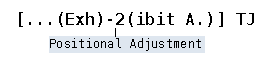
\includegraphics[width=2in]{tj.pdf}
    \caption{The TJ text showing operator, which specifies the glyphs to render and, by reference to a font object (not shown), their widths, along with any associated positional adjustments, given in text space units.}\label{fig:tj}
\end{figure}

The significant discovery of \emph{Story Beyond the Eye} was the existence and utilization of a novel redacted text information leak.
PDF documents can render text in numerous ways, including by use of a text showing operator, one of which (TJ) is depicted in Figure~\ref{fig:tj}. 
The TJ operator takes as arguments a string of text and a vector of \emph{positional adjustments} which displace the character with respect to a default position. 
This default position is usually a fixed offset from the previous character equivalent to the \emph{advance width} of the previous character defined elsewhere in the PDF document.

Glyph advance widths and glyph shifts create a security concern, and \emph{Story Beyond the Eye} found that most PDF redaction tools replace text selected for redaction with a single large shift of the same width as the redacted text showing operator, creating the two significant security risks:
\begin{itemize}
	\item The precise width of the redaction can be used to eliminate potential redacted texts, and is made more distinct than advance widths alone by glyph shifts.
	\item Any non-redacted glyph shifts conditioned on redacted glyphs can be used to eliminate potential redacted texts.
\end{itemize}
The work also addressed concerns related to nonexcising redactions. 
These redactions are cases where the text underneath the redaction can be selected and copied to the system clipboard from the PDF document.

Glyph shifts may then be classified as \emph{independent} or \emph{dependent}, where the former implies they are not determined by any particular character in the document, and the latter implies that they are---this is precisely dangerous if the character they are conditioned on is redacted.
This itself is not dangerous if the amount of information leaked on redacted text is small or the redaction tools themselves remove this information.
Thus, the methodology of the paper was split into extracting and evaluating glyph shifting schemes, e.g. from Microsoft Word's ``Save-as-PDF'' feature, and evaluating the information removed by redaction tools.

The latter corresponded to an evaluation of what types of information the redaction tools leaked, and after reverse engineering the schemes produced by 11 redaction tools, including Adobe Acrobat, the paper finds \emph{none} but those that rasterize the document entirely sufficiently mitigate these leaks.
Two of the tools were completely broken, and did not remove the text at all (created nonexcising redactions): the present author notified them of this problem and as a result of this both the tools have published patches.

\lstset{ %
language=C++,                % choose the language of the code
basicstyle=\ttfamily\footnotesize,       % the size of the fonts that are used for the code
numbers=left,                   % where to put the line-numbers
numberstyle=\footnotesize,      % the size of the fonts that are used for the line-numbers
stepnumber=1,                   % the step between two line-numbers. If it is 1 each line will be numbered
numbersep=5pt,                  % how far the line-numbers are from the code
backgroundcolor=\color{white},  % choose the background color. You must add \usepackage{color}
showspaces=false,               % show spaces adding particular underscores
showstringspaces=false,         % underline spaces within strings
showtabs=false,                 % show tabs within strings adding particular underscores
frame=single,           % adds a frame around the code
tabsize=2,          % sets default tabsize to 2 spaces
captionpos=b,           % sets the caption-position to bottom
breaklines=true,        % sets automatic line breaking
breakatwhitespace=false,    % sets if automatic breaks should only happen at whitespace
escapeinside={\%*}{*)}          % if you want to add a comment within your code
}

\begin{figure}
\begin{lstlisting}
for (int j = i + 1; j < vs->size(); j++) {
    t = ttfScaledWidths[j] / 1000;
    d = internalMSWordWidths[j] / internalMSWordFontSize;
    ttf += t;
    msWord += d;
    disp = ttf - msWord;
    if (((disp > 0.003) || (disp < -0.003)) && i != vs->size() - 1) {
      int adj = disp * 1000 + 0.5;
      vs->setShift(j, adj);
      ttf = msWord = 0;
    } else {
      vs->setShift(j, 0);
    }
}
\end{lstlisting}
\caption{Snippet of reverse engineered code representing how Microsoft Word leaks redacted character information into non-redacted characters in a PDF document.
    }
\label{fig:msword-snippet}
\end{figure}

The extraction and evaluation of the glyph shifting schemes involved precise tracing of PDF producer software and reverse engineering to extract an exact model of their positioning algorithms for text. 
Microsoft Word, in particular, provided glyph shift values that were \emph{highly} dependent on redacted glyphs, due to a floating-point error accumulation algorithm that compares the ``real'' PDF position of a glyph with a set of artificial positions determined by the full text of a given line.
A portion of this behavior, one of the error accumulators, is presented in Fig.~\ref{fig:msword-snippet}.
Note the internal widths used on line 3 of the figure are determined by a loop with no overflow reset and the redacted information held by the accumulator is not zero after a single shift is written: this detail is given in the publication's appendix.

The extraction of the prior algoithm and reverse engineering of PDF producer structures in a rich area and was not given sufficient space due to constraints on the original publication.
The proposed dissertation would provide both an explanation of how these algorithms were extracted as well as some of the challenges and solutions developed when addressing the problems of discovering and breaking redactions, and classifying glyph shifting schemes.

\subsubsection{Evaluation}

\paragraph{Synthetic Evaluation.}
The evaluation of the vulnerability these shifting schemes create for redacted text was based on the simulation of redactions on text from the New York Times annotated corpus~\cite{nytCorp} using various \emph{dictionaries}.
This represents how the amount of information leaked depends on prior information about the redacted text. 
For example, if we know the redacted text is one of 151,671 American surnames, then this redaction leaks at most $log_{2}(151, 671) \approx 17.2$ bits. 
Notably, these dictionaries included:



\renewcommand{\qedsymbol}{\rule{7pt}{7pt}}
\newcommand\maxray{Edact-Ray}

% The following macros give the pretty names of texts dictionaries and fonts.

\newcommand\wkpname{Wikipedia}
\newcommand\lawname{Legal}
\newcommand\nytname{News}

\newcommand\strname{Str}
\newcommand\acrnname{Acrn}
\newcommand\pronname{Pron}
\newcommand\wordname{Word}
\newcommand\fnname{FN}
\newcommand\lnname{LN}
\newcommand\filnname{FILN}
\newcommand\fixlnname{FI$\times$LN}
\newcommand\fnlnname{FNLN}
\newcommand\fnxlnname{FN$\times$LN}
\newcommand\ctryname{Ctry}
\newcommand\rgnname{Rgn}
\newcommand\natlname{Natl}

\newcommand\tfontname{Times}
\newcommand\afontname{Arial}
\newcommand\bfontname{Calibri}
\newcommand\rfontname{Courier}

\newcommand\nadjname{Unadjusted}
\newcommand\wxiiname{Word 2007}
\newcommand\wxxiname{Word 2021}

\newcommand\nadjshortname{Un}
\newcommand\wxiishortname{W07}
\newcommand\wxxishortname{W19}

\newcommand\uniname{Uniformly distributed}
\newcommand\empname{Text frequency distr.}

\newcommand\msWordPrefixMatch{XXX}

% wild section results
\newcommand\numWildCorpora{4}
\newcommand\numWildDNSALocSample{400}
\newcommand\numWildFOIALocSample{100}
\newcommand\numWildGovtLocSample{400}
\newcommand\numWildRECAPLocSample{100}
\newcommand\numWildLocSample{1,000}

\newcommand\dnsaNumDocs{678}
\newcommand\foiaNumDocs{1,580}
\newcommand\govtNumDocs{3,145}
\newcommand\recapNumDocs{\num{2.5e4}}
\newcommand\oigNumDocs{\num{1.9e4}}
% \newcommand\oigNumDocs{18,975}

% \newcommand\recapNumDocs{24,835}

\newcommand\dnsaPg{\num{1.2e4}}
% \newcommand\dnsaPg{12,498}
\newcommand\foiaPg{\num{4.9e5}}
% \newcommand\foiaPg{491,782}
\newcommand\oigPg{\num{5.2e5}}
% \newcommand\oigPg{515,870}
% \newcommand\govtPg{491,782}
\newcommand\recapPg{\num{3.4e5}}
% \newcommand\recapPg{336,973}

\newcommand\dnsaNonRastPg{8,628}
\newcommand\foiaNonRastPg{12,012}
\newcommand\govtNonRastPg{259,939}
\newcommand\recapNonRastPg{269,546}

% select corpus_name, count(distinct document_name) from redactions join pages
% on redactions.page = pages.hash group by corpus_name;
\newcommand\dnsaNumDocsWRedact{7}
\newcommand\foiaNumDocsWRedact{296}
\newcommand\govtNumDocsWRedact{230}
\newcommand\recapNumDocsWRedact{67}
\newcommand\totNumDocsWRedact{600}

\newcommand\totNumPagesWRedact{11,997}

% 112,149,773
\newcommand\numRECAPpages{$\approx10^{8}$}

\newcommand\avgShortlist{801}
\newcommand\avgNumNames{238}
\newcommand\avgStdDevRECAPName{1.3}

\newcommand\totalNonSynthNames{778}
\newcommand\numNonSynthRedactions{5,282}

\newcommand\numWildAttacked{769}

% select corpus_name, count(distinct redactions.id) from redactions 
% join pages on redactions.page = pages.hash group by corpus_name;
\newcommand\dnsaMetaRedact{235}
\newcommand\foiaMetaRedact{\num{4.5e4}}
\newcommand\oigMetaRedact{\num{1.3e4}}
% \newcommand\foiaMetaRedact{45,219}
% \newcommand\oigMetaRedact{13,214}
\newcommand\govtMetaRedact{51,651}
\newcommand\recapMetaRedact{1,221}
\newcommand\totMetaRedact{80,301}

\newcommand\unadjDNSA{7}
\newcommand\unadjFOIA{422}
\newcommand\unadjGOVT{2,589}
\newcommand\unadjRECAP{7}

\newcommand\ocrDNSA{0}
\newcommand\ocrFOIA{16,678}
\newcommand\ocrGOVT{3,939}
\newcommand\ocrRECAP{224}

\newcommand\mswDNSAExact{14}
\newcommand\mswFOIAExact{3}
\newcommand\mswGOVTExact{4,712}
\newcommand\mswRECAPExact{119}
\newcommand\mswDNSAExactFivePerc{7}
\newcommand\mswFOIAExactFivePerc{1}
\newcommand\mswGOVTExactFivePerc{1,428}
\newcommand\mswRECAPExactFivePerc{0}

\newcommand\mswDNSAExactTwelve{14}
\newcommand\mswDNSAExactTwenty{7}
\newcommand\mswFOIAExactTwelve{3}
\newcommand\mswFOIAExactTwenty{0}
\newcommand\mswGOVTExactTwelve{4,425}
\newcommand\mswGOVTExactTwenty{967}
\newcommand\mswRECAPExactTwelve{112}
\newcommand\mswRECAPExactTwenty{53}

\newcommand\mswDNSANear{3}
\newcommand\mswFOIANear{2}
\newcommand\mswGOVTNear{177}
\newcommand\mswRECAPNear{33}
\newcommand\mswDNSANearTwelve{0}
\newcommand\mswDNSANearTwenty{3}
\newcommand\mswFOIANearTwelve{1}
\newcommand\mswFOIANearTwenty{2}
\newcommand\mswGOVTNearTwelve{132}
\newcommand\mswGOVTNearTwenty{49}
\newcommand\mswRECAPNearTwelve{33}
\newcommand\mswRECAPNearTwenty{0}

\newcommand\unrecDNSA{214}
\newcommand\unrecDNSAUnkFont{32}
\newcommand\unrecDNSAKnwFont{182}
\newcommand\unrecFOIA{\num{1.3e4}}
% \newcommand\unrecFOIA{13,214}
\newcommand\unrecFOIAUnkFont{982}
\newcommand\unrecFOIAKnwFont{9,108}
\newcommand\unrecGOVT{40,270}
\newcommand\unrecGOVTUnkFont{6,468}
\newcommand\unrecGOVTKnwFont{33,802}
\newcommand\unrecRECAP{838}
\newcommand\unrecRECAPUnkFont{183}
\newcommand\unrecRECAPKnwFont{655}
\newcommand\unrecOIG{\num{1e4}}
% \newcommand\unrecOIG{10,517}

\newcommand\numWildTotalVuln{4,848}

\newcommand\nameDictSize{235,560}

\newcommand\numOIGUnmatched{39}

\newcommand\numRECAPPDFs{11,181,433}
\newcommand\numRECAPredactions{195,436}
\newcommand\numRECAPNameredactions{6,541}
\newcommand\numRECAPredactionDocs{710}

\newcommand\numRECAPnadj{327}
\newcommand\numRECAPnadjSample{100}
\newcommand\numRECAPocr{445}
\newcommand\numRECAPmsw{58}
\newcommand\numRECAPunk{5,691}
\newcommand\numRECAPNearMSW{20}

\newcommand\numRECAPtrivialRedaction{\num{1.9e5}}
%\newcommand\numRECAPtrivialRedaction{193,714}

\newcommand\nameDictSizeComb{7,066,800}

% ---
% Wild Results
% ---
\newcommand\dnsaExactName{XXX}
\newcommand\dnsaExactMrName{XXX}
\newcommand\dnsaExactMrsName{XXX}
\newcommand\dnsaExactFiLn{XXX}

\newcommand\foiaExactName{XXX}
\newcommand\foiaExactMrName{XXX}
\newcommand\foiaExactMrsName{XXX}
\newcommand\foiaExactFiLn{XXX}

\newcommand\govtExactName{XXX}
\newcommand\govtExactMrName{XXX}
\newcommand\govtExactMrsName{XXX}
\newcommand\govtExactFiLn{XXX}

\newcommand\recapExactName{XXX}
\newcommand\recapExactMrName{XXX}
\newcommand\recapExactMrsName{XXX}
\newcommand\recapExactFiLn{XXX}

\newcommand\hybridNadjAvgMatches{5,861}
\newcommand\hybridNadjMinMatches{10}

\newcommand\numFOIANamesAttacked{711}
\newcommand\numOIGNamesAttacked{58}

\newcommand\numFOIAUnmatched{382}
\newcommand\numFOIAUniq{3}
\newcommand\numOIGUniq{0}
\newcommand\numFOIAavg{2,435}
\newcommand\numFOIAmed{494}
\newcommand\numOIGavg{4,260}
\newcommand\numOIGmed{1,081}

\newcommand\foiaNameMaxRank{125,282}

\newcommand\avgMatchesWildTwo{561.09}
\newcommand\ratioNamesToMatches{420}
\newcommand\ratioWidthClassesToWidths{1095}

% ---
% Epstein Case Study
% ---

\newcommand\numEpsteinPagesRedacted{15}
\newcommand\numEpsteinDocuments{23}
\newcommand\numEpsteinRedactions{62}
\newcommand\numEpsteinVulnRedactions{4}


% The following macros give the dictionary sizes and uniform entropies. The names have
% the form
% 
%     \neltDDD  and  \hxDDD
% 
% where DDD is the dictionary, one of str, acrn, pron, word, fn, ln, filn, fnln, ctry, rgn, or natl


\newcommand\neltword{63,054} % dict rev. unk
\newcommand\hxword{15.9} % dict rev. unk
\newcommand\neltpron{10} % dict rev. unk
\newcommand\hxpron{3.3} % dict rev. unk
\newcommand\neltfn{100,364} % dict rev. unk
\newcommand\hxfn{16.6} % dict rev. unk
\newcommand\neltln{151,671} % dict rev. unk
\newcommand\hxln{17.2} % dict rev. unk
\newcommand\neltfi{26} % dict rev. unk
\newcommand\hxfi{4.7} % dict rev. unk
\newcommand\neltctry{566} % dict rev. unk
\newcommand\hxctry{9.1} % dict rev. unk
\newcommand\neltrgn{2,794,808} % dict rev. unk
\newcommand\hxrgn{21.4} % dict rev. unk
\newcommand\neltnatl{509} % dict rev. unk
\newcommand\hxnatl{9.0} % dict rev. unk
\newcommand\neltfiln{3,943,446} % dict rev. unk
\newcommand\hxfiln{21.9} % dict rev. unk
\newcommand\neltfnln{15,222,308,244} % dict rev. unk/unk
\newcommand\hxfnln{33.8} % dict rev. unk/unk
\newcommand\hxtsfnln{20.8} % dict rev. unk/unk
\newcommand\neltstr{90,706,185,230,812,058,042,928}
\newcommand\hxstr{76.3}
\newcommand\neltacrn{12,356,604}
\newcommand\hxacrn{23.6}
 % python tools/mkdefs0.py
% Overrides for prettier formatting. Always compare to actual numbers in defs0.tex.

\renewcommand\neltacrn{\num{1.2e7}}
\renewcommand\neltstr{\num{9e22}}
\renewcommand\neltfiln{\num{3.9e6}}
\renewcommand\neltfnln{\num{1.5e10}}
\renewcommand\neltrgn{\num{2.8e6}}
\newcommand\nelttsfnln{\num{1.8e6}}

% The following macros are for the word counts for each dictionary with respect to given
% text and the entropy of the dictionary distribution w.r.t. to a text. The names have
% the form
% 
%     \noccTTTDDD  and  \hxTTTDDD
% 
% where:
% 
% TTT is the text, one of wkp (Wikipedia), law (Legal), or nyt (News)
% DDD is the dictionary, one of str, acrn, pron, word, fn, ln, filn, fnln, ctry, rgn, or natl

\newcommand\noccnytword{432,896,070} % dict rev. unk, cnts rev. unk
\newcommand\hxnytword{12.3} % dict rev. unk, cnts rev. unk
\newcommand\noccnytpron{21,049,889} % dict rev. unk, cnts rev. unk
\newcommand\hxnytpron{2.8} % dict rev. unk, cnts rev. unk
\newcommand\noccnytfn{71,031,188} % dict rev. unk, cnts rev. unk
\newcommand\hxnytfn{9.6} % dict rev. unk, cnts rev. unk
\newcommand\noccnytln{97,551,697} % dict rev. unk, cnts rev. unk
\newcommand\hxnytln{10.7} % dict rev. unk, cnts rev. unk
\newcommand\noccnytfiln{2,139,713} % cnts rev. unk
\newcommand\hxnytfiln{14.7} % cnts rev. unk
\newcommand\noccnytfnln{14,440,238} % cnts rev. unk
\newcommand\hxnytfnln{16.0} % cnts rev. unk
\newcommand\noccnyttsfnln{822,189} % cnts rev. unk
\newcommand\hxnyttsfnln{12.6} % cnts rev. unk
\newcommand\noccnytctry{3,905,371} % cnts rev. unk
\newcommand\hxnytctry{5.9} % cnts rev. unk
\newcommand\noccnytrgn{33,636,150} % cnts rev. unk
\newcommand\hxnytrgn{10.6} % cnts rev. unk
\newcommand\noccnytnatl{4,081,019} % cnts rev. unk
\newcommand\hxnytnatl{5.4} % cnts rev. unk
\newcommand\noccnytstr{791,209,093} % cnts rev. unk
\newcommand\hxnytstr{11.8} % cnts rev. unk
\newcommand\noccnytacrn{4,674,379} % cnts rev. unk
\newcommand\hxnytacrn{10.0} % cnts rev. unk
 % python tools/mkdefs1.py

% The following macros are the results of the simulated redaction and guessing experiment. The
% names have the form
% 
%     \SSSMMMTTTDDDWWWFZ
% 
% where:
% 
% SSS is the statistic, one of hyu, hyw, hxyu, hxyw, puu, puw, pgu, pgw
% MMM is the static modifier, omitted or one of min, max, or avg
% TTT is the text, one of any (Any, unadj only), wkp (Wikipedia), law (Legal), or nyt (News)
% DDD is the dictionary, one of str, acrn, pron, word, fn, ln, filn, fnln, ctry, rgn, or natl
% WWW is the workflow, one of nadj (Unajusted), wxii (Word 2012), or wxxi (Word 2021)
% F is the font, one of t (Times), b (Calibri), a (Arial), or r (Courier)
% Z is the font size, one of ix (9 pt), x (10 pt), xi (11 pt), or xii (12 pt)
% 
% For example, \hyuavgnytfnnadjrxii is the average document residual entropy H(Y) for redactions
% on the News (NYT) corpus with first name dictionary, unadjusted text in 12 pt Courier.

\newcommand\hyunytlnnadjbx{12.7} % dict rev. unk
\newcommand\puupctnytlnnadjbx{\textless1\%} % dict rev. unk
\newcommand\pgupctnytlnnadjbx{6\%} % dict rev. unk
\newcommand\gyunytlnnadjbx{278} % dict rev. unk
\newcommand\hyunytlnnadjbxii{12.7} % dict rev. unk
\newcommand\puupctnytlnnadjbxii{\textless1\%} % dict rev. unk
\newcommand\pgupctnytlnnadjbxii{6\%} % dict rev. unk
\newcommand\gyunytlnnadjbxii{278} % dict rev. unk
\newcommand\hywnytlnnadjbx{9.9} % dict rev. unk, cnt rev. unk
\newcommand\puwpctnytlnnadjbx{5\%} % dict rev. unk, cnt rev. unk
\newcommand\pgwpctnytlnnadjbx{84\%} % dict rev. unk, cnt rev. unk
\newcommand\gywnytlnnadjbx{7} % dict rev. unk, cnt rev. unk
\newcommand\hywnytlnnadjbxii{9.9} % dict rev. unk, cnt rev. unk
\newcommand\puwpctnytlnnadjbxii{5\%} % dict rev. unk, cnt rev. unk
\newcommand\pgwpctnytlnnadjbxii{84\%} % dict rev. unk, cnt rev. unk
\newcommand\gywnytlnnadjbxii{7} % dict rev. unk, cnt rev. unk
\newcommand\hyunytlnnadjax{8.3} % dict rev. unk
\newcommand\puupctnytlnnadjax{\textless1\%} % dict rev. unk
\newcommand\pgupctnytlnnadjax{\textless1\%} % dict rev. unk
\newcommand\gyunytlnnadjax{12} % dict rev. unk
\newcommand\hyunytlnnadjaxii{8.3} % dict rev. unk
\newcommand\puupctnytlnnadjaxii{\textless1\%} % dict rev. unk
\newcommand\pgupctnytlnnadjaxii{\textless1\%} % dict rev. unk
\newcommand\gyunytlnnadjaxii{12} % dict rev. unk
\newcommand\hywnytlnnadjax{7.4} % dict rev. unk, cnt rev. unk
\newcommand\puwpctnytlnnadjax{\textless1\%} % dict rev. unk, cnt rev. unk
\newcommand\pgwpctnytlnnadjax{46\%} % dict rev. unk, cnt rev. unk
\newcommand\gywnytlnnadjax{4} % dict rev. unk, cnt rev. unk
\newcommand\hywnytlnnadjaxii{7.4} % dict rev. unk, cnt rev. unk
\newcommand\puwpctnytlnnadjaxii{\textless1\%} % dict rev. unk, cnt rev. unk
\newcommand\pgwpctnytlnnadjaxii{46\%} % dict rev. unk, cnt rev. unk
\newcommand\gywnytlnnadjaxii{4} % dict rev. unk, cnt rev. unk
\newcommand\hyunytlnnadjrx{2.9} % dict rev. unk
\newcommand\puupctnytlnnadjrx{\textless1\%} % dict rev. unk
\newcommand\pgupctnytlnnadjrx{\textless1\%} % dict rev. unk
\newcommand\gyunytlnnadjrx{1} % dict rev. unk
\newcommand\hyunytlnnadjrxii{2.9} % dict rev. unk
\newcommand\puupctnytlnnadjrxii{\textless1\%} % dict rev. unk
\newcommand\pgupctnytlnnadjrxii{\textless1\%} % dict rev. unk
\newcommand\gyunytlnnadjrxii{1} % dict rev. unk
\newcommand\hywnytlnnadjrx{2.9} % dict rev. unk, cnt rev. unk
\newcommand\puwpctnytlnnadjrx{\textless1\%} % dict rev. unk, cnt rev. unk
\newcommand\pgwpctnytlnnadjrx{14\%} % dict rev. unk, cnt rev. unk
\newcommand\gywnytlnnadjrx{1} % dict rev. unk, cnt rev. unk
\newcommand\hywnytlnnadjrxii{2.9} % dict rev. unk, cnt rev. unk
\newcommand\puwpctnytlnnadjrxii{\textless1\%} % dict rev. unk, cnt rev. unk
\newcommand\pgwpctnytlnnadjrxii{14\%} % dict rev. unk, cnt rev. unk
\newcommand\gywnytlnnadjrxii{1} % dict rev. unk, cnt rev. unk
\newcommand\hyunytlnnadjtx{8.2} % dict rev. unk
\newcommand\puupctnytlnnadjtx{\textless1\%} % dict rev. unk
\newcommand\pgupctnytlnnadjtx{\textless1\%} % dict rev. unk
\newcommand\gyunytlnnadjtx{11} % dict rev. unk
\newcommand\hyunytlnnadjtxii{8.2} % dict rev. unk
\newcommand\puupctnytlnnadjtxii{\textless1\%} % dict rev. unk
\newcommand\pgupctnytlnnadjtxii{\textless1\%} % dict rev. unk
\newcommand\gyunytlnnadjtxii{11} % dict rev. unk
\newcommand\hywnytlnnadjtx{7.4} % dict rev. unk, cnt rev. unk
\newcommand\puwpctnytlnnadjtx{\textless1\%} % dict rev. unk, cnt rev. unk
\newcommand\pgwpctnytlnnadjtx{47\%} % dict rev. unk, cnt rev. unk
\newcommand\gywnytlnnadjtx{5} % dict rev. unk, cnt rev. unk
\newcommand\hywnytlnnadjtxii{7.4} % dict rev. unk, cnt rev. unk
\newcommand\puwpctnytlnnadjtxii{\textless1\%} % dict rev. unk, cnt rev. unk
\newcommand\pgwpctnytlnnadjtxii{47\%} % dict rev. unk, cnt rev. unk
\newcommand\gywnytlnnadjtxii{5} % dict rev. unk, cnt rev. unk
\newcommand\hyunytpronnadjbx{3.3} % dict rev. unk
\newcommand\puupctnytpronnadjbx{10\%} % dict rev. unk
\newcommand\pgupctnytpronnadjbx{100\%} % dict rev. unk
\newcommand\gyunytpronnadjbx{1} % dict rev. unk
\newcommand\hyunytpronnadjbxii{3.3} % dict rev. unk
\newcommand\puupctnytpronnadjbxii{10\%} % dict rev. unk
\newcommand\pgupctnytpronnadjbxii{100\%} % dict rev. unk
\newcommand\gyunytpronnadjbxii{1} % dict rev. unk
\newcommand\hywnytpronnadjbx{2.8} % dict rev. unk, cnt rev. unk
\newcommand\puwpctnytpronnadjbx{100\%} % dict rev. unk, cnt rev. unk
\newcommand\pgwpctnytpronnadjbx{100\%} % dict rev. unk, cnt rev. unk
\newcommand\gywnytpronnadjbx{1} % dict rev. unk, cnt rev. unk
\newcommand\hywnytpronnadjbxii{2.8} % dict rev. unk, cnt rev. unk
\newcommand\puwpctnytpronnadjbxii{100\%} % dict rev. unk, cnt rev. unk
\newcommand\pgwpctnytpronnadjbxii{100\%} % dict rev. unk, cnt rev. unk
\newcommand\gywnytpronnadjbxii{1} % dict rev. unk, cnt rev. unk
\newcommand\hyunytpronnadjax{3.1} % dict rev. unk
\newcommand\puupctnytpronnadjax{10\%} % dict rev. unk
\newcommand\pgupctnytpronnadjax{90\%} % dict rev. unk
\newcommand\gyunytpronnadjax{1} % dict rev. unk
\newcommand\hyunytpronnadjaxii{3.1} % dict rev. unk
\newcommand\puupctnytpronnadjaxii{10\%} % dict rev. unk
\newcommand\pgupctnytpronnadjaxii{90\%} % dict rev. unk
\newcommand\gyunytpronnadjaxii{1} % dict rev. unk
\newcommand\hywnytpronnadjax{2.8} % dict rev. unk, cnt rev. unk
\newcommand\puwpctnytpronnadjax{88\%} % dict rev. unk, cnt rev. unk
\newcommand\pgwpctnytpronnadjax{100\%} % dict rev. unk, cnt rev. unk
\newcommand\gywnytpronnadjax{1} % dict rev. unk, cnt rev. unk
\newcommand\hywnytpronnadjaxii{2.8} % dict rev. unk, cnt rev. unk
\newcommand\puwpctnytpronnadjaxii{88\%} % dict rev. unk, cnt rev. unk
\newcommand\pgwpctnytpronnadjaxii{100\%} % dict rev. unk, cnt rev. unk
\newcommand\gywnytpronnadjaxii{1} % dict rev. unk, cnt rev. unk
\newcommand\hyunytpronnadjrx{2.0} % dict rev. unk
\newcommand\puupctnytpronnadjrx{40\%} % dict rev. unk
\newcommand\pgupctnytpronnadjrx{50\%} % dict rev. unk
\newcommand\gyunytpronnadjrx{1} % dict rev. unk
\newcommand\hyunytpronnadjrxii{2.0} % dict rev. unk
\newcommand\puupctnytpronnadjrxii{40\%} % dict rev. unk
\newcommand\pgupctnytpronnadjrxii{50\%} % dict rev. unk
\newcommand\gyunytpronnadjrxii{1} % dict rev. unk
\newcommand\hywnytpronnadjrx{1.9} % dict rev. unk, cnt rev. unk
\newcommand\puwpctnytpronnadjrx{38\%} % dict rev. unk, cnt rev. unk
\newcommand\pgwpctnytpronnadjrx{73\%} % dict rev. unk, cnt rev. unk
\newcommand\gywnytpronnadjrx{1} % dict rev. unk, cnt rev. unk
\newcommand\hywnytpronnadjrxii{1.9} % dict rev. unk, cnt rev. unk
\newcommand\puwpctnytpronnadjrxii{38\%} % dict rev. unk, cnt rev. unk
\newcommand\pgwpctnytpronnadjrxii{73\%} % dict rev. unk, cnt rev. unk
\newcommand\gywnytpronnadjrxii{1} % dict rev. unk, cnt rev. unk
\newcommand\hyunytpronnadjtx{3.3} % dict rev. unk
\newcommand\puupctnytpronnadjtx{10\%} % dict rev. unk
\newcommand\pgupctnytpronnadjtx{100\%} % dict rev. unk
\newcommand\gyunytpronnadjtx{1} % dict rev. unk
\newcommand\hyunytpronnadjtxii{3.3} % dict rev. unk
\newcommand\puupctnytpronnadjtxii{10\%} % dict rev. unk
\newcommand\pgupctnytpronnadjtxii{100\%} % dict rev. unk
\newcommand\gyunytpronnadjtxii{1} % dict rev. unk
\newcommand\hywnytpronnadjtx{2.8} % dict rev. unk, cnt rev. unk
\newcommand\puwpctnytpronnadjtx{100\%} % dict rev. unk, cnt rev. unk
\newcommand\pgwpctnytpronnadjtx{100\%} % dict rev. unk, cnt rev. unk
\newcommand\gywnytpronnadjtx{1} % dict rev. unk, cnt rev. unk
\newcommand\hywnytpronnadjtxii{2.8} % dict rev. unk, cnt rev. unk
\newcommand\puwpctnytpronnadjtxii{100\%} % dict rev. unk, cnt rev. unk
\newcommand\pgwpctnytpronnadjtxii{100\%} % dict rev. unk, cnt rev. unk
\newcommand\gywnytpronnadjtxii{1} % dict rev. unk, cnt rev. unk
\newcommand\hyunytwordnadjbx{12.8} % dict rev. unk
\newcommand\puupctnytwordnadjbx{\textless1\%} % dict rev. unk
\newcommand\pgupctnytwordnadjbx{16\%} % dict rev. unk
\newcommand\gyunytwordnadjbx{310} % dict rev. unk
\newcommand\hyunytwordnadjbxii{12.8} % dict rev. unk
\newcommand\puupctnytwordnadjbxii{\textless1\%} % dict rev. unk
\newcommand\pgupctnytwordnadjbxii{16\%} % dict rev. unk
\newcommand\gyunytwordnadjbxii{310} % dict rev. unk
\newcommand\hywnytwordnadjbx{11.2} % dict rev. unk, cnt rev. unk
\newcommand\puwpctnytwordnadjbx{4\%} % dict rev. unk, cnt rev. unk
\newcommand\pgwpctnytwordnadjbx{74\%} % dict rev. unk, cnt rev. unk
\newcommand\gywnytwordnadjbx{43} % dict rev. unk, cnt rev. unk
\newcommand\hywnytwordnadjbxii{11.2} % dict rev. unk, cnt rev. unk
\newcommand\puwpctnytwordnadjbxii{4\%} % dict rev. unk, cnt rev. unk
\newcommand\pgwpctnytwordnadjbxii{74\%} % dict rev. unk, cnt rev. unk
\newcommand\gywnytwordnadjbxii{43} % dict rev. unk, cnt rev. unk
\newcommand\hyunytwordnadjax{8.7} % dict rev. unk
\newcommand\puupctnytwordnadjax{\textless1\%} % dict rev. unk
\newcommand\pgupctnytwordnadjax{2\%} % dict rev. unk
\newcommand\gyunytwordnadjax{15} % dict rev. unk
\newcommand\hyunytwordnadjaxii{8.7} % dict rev. unk
\newcommand\puupctnytwordnadjaxii{\textless1\%} % dict rev. unk
\newcommand\pgupctnytwordnadjaxii{2\%} % dict rev. unk
\newcommand\gyunytwordnadjaxii{15} % dict rev. unk
\newcommand\hywnytwordnadjax{7.9} % dict rev. unk, cnt rev. unk
\newcommand\puwpctnytwordnadjax{\textless1\%} % dict rev. unk, cnt rev. unk
\newcommand\pgwpctnytwordnadjax{27\%} % dict rev. unk, cnt rev. unk
\newcommand\gywnytwordnadjax{8} % dict rev. unk, cnt rev. unk
\newcommand\hywnytwordnadjaxii{7.9} % dict rev. unk, cnt rev. unk
\newcommand\puwpctnytwordnadjaxii{\textless1\%} % dict rev. unk, cnt rev. unk
\newcommand\pgwpctnytwordnadjaxii{27\%} % dict rev. unk, cnt rev. unk
\newcommand\gywnytwordnadjaxii{8} % dict rev. unk, cnt rev. unk
\newcommand\hyunytwordnadjrx{3.3} % dict rev. unk
\newcommand\puupctnytwordnadjrx{\textless1\%} % dict rev. unk
\newcommand\pgupctnytwordnadjrx{\textless1\%} % dict rev. unk
\newcommand\gyunytwordnadjrx{1} % dict rev. unk
\newcommand\hyunytwordnadjrxii{3.3} % dict rev. unk
\newcommand\puupctnytwordnadjrxii{\textless1\%} % dict rev. unk
\newcommand\pgupctnytwordnadjrxii{\textless1\%} % dict rev. unk
\newcommand\gyunytwordnadjrxii{1} % dict rev. unk
\newcommand\hywnytwordnadjrx{3.2} % dict rev. unk, cnt rev. unk
\newcommand\puwpctnytwordnadjrx{\textless1\%} % dict rev. unk, cnt rev. unk
\newcommand\pgwpctnytwordnadjrx{6\%} % dict rev. unk, cnt rev. unk
\newcommand\gywnytwordnadjrx{1} % dict rev. unk, cnt rev. unk
\newcommand\hywnytwordnadjrxii{3.2} % dict rev. unk, cnt rev. unk
\newcommand\puwpctnytwordnadjrxii{\textless1\%} % dict rev. unk, cnt rev. unk
\newcommand\pgwpctnytwordnadjrxii{6\%} % dict rev. unk, cnt rev. unk
\newcommand\gywnytwordnadjrxii{1} % dict rev. unk, cnt rev. unk
\newcommand\hyunytwordnadjtx{8.7} % dict rev. unk
\newcommand\puupctnytwordnadjtx{\textless1\%} % dict rev. unk
\newcommand\pgupctnytwordnadjtx{2\%} % dict rev. unk
\newcommand\gyunytwordnadjtx{16} % dict rev. unk
\newcommand\hyunytwordnadjtxii{8.7} % dict rev. unk
\newcommand\puupctnytwordnadjtxii{\textless1\%} % dict rev. unk
\newcommand\pgupctnytwordnadjtxii{2\%} % dict rev. unk
\newcommand\gyunytwordnadjtxii{16} % dict rev. unk
\newcommand\hywnytwordnadjtx{8.1} % dict rev. unk, cnt rev. unk
\newcommand\puwpctnytwordnadjtx{\textless1\%} % dict rev. unk, cnt rev. unk
\newcommand\pgwpctnytwordnadjtx{29\%} % dict rev. unk, cnt rev. unk
\newcommand\gywnytwordnadjtx{9} % dict rev. unk, cnt rev. unk
\newcommand\hywnytwordnadjtxii{8.1} % dict rev. unk, cnt rev. unk
\newcommand\puwpctnytwordnadjtxii{\textless1\%} % dict rev. unk, cnt rev. unk
\newcommand\pgwpctnytwordnadjtxii{29\%} % dict rev. unk, cnt rev. unk
\newcommand\gywnytwordnadjtxii{9} % dict rev. unk, cnt rev. unk
\newcommand\hyunytfnnadjbx{12.3} % dict rev. unk
\newcommand\puupctnytfnnadjbx{\textless1\%} % dict rev. unk
\newcommand\pgupctnytfnnadjbx{8\%} % dict rev. unk
\newcommand\gyunytfnnadjbx{209} % dict rev. unk
\newcommand\hyunytfnnadjbxii{12.3} % dict rev. unk
\newcommand\puupctnytfnnadjbxii{\textless1\%} % dict rev. unk
\newcommand\pgupctnytfnnadjbxii{8\%} % dict rev. unk
\newcommand\gyunytfnnadjbxii{209} % dict rev. unk
\newcommand\hywnytfnnadjbx{9.2} % dict rev. unk, cnt rev. unk
\newcommand\puwpctnytfnnadjbx{14\%} % dict rev. unk, cnt rev. unk
\newcommand\pgwpctnytfnnadjbx{89\%} % dict rev. unk, cnt rev. unk
\newcommand\gywnytfnnadjbx{3} % dict rev. unk, cnt rev. unk
\newcommand\hywnytfnnadjbxii{9.2} % dict rev. unk, cnt rev. unk
\newcommand\puwpctnytfnnadjbxii{14\%} % dict rev. unk, cnt rev. unk
\newcommand\pgwpctnytfnnadjbxii{89\%} % dict rev. unk, cnt rev. unk
\newcommand\gywnytfnnadjbxii{3} % dict rev. unk, cnt rev. unk
\newcommand\hyunytfnnadjax{7.9} % dict rev. unk
\newcommand\puupctnytfnnadjax{\textless1\%} % dict rev. unk
\newcommand\pgupctnytfnnadjax{\textless1\%} % dict rev. unk
\newcommand\gyunytfnnadjax{9} % dict rev. unk
\newcommand\hyunytfnnadjaxii{7.9} % dict rev. unk
\newcommand\puupctnytfnnadjaxii{\textless1\%} % dict rev. unk
\newcommand\pgupctnytfnnadjaxii{\textless1\%} % dict rev. unk
\newcommand\gyunytfnnadjaxii{9} % dict rev. unk
\newcommand\hywnytfnnadjax{7.0} % dict rev. unk, cnt rev. unk
\newcommand\puwpctnytfnnadjax{\textless1\%} % dict rev. unk, cnt rev. unk
\newcommand\pgwpctnytfnnadjax{52\%} % dict rev. unk, cnt rev. unk
\newcommand\gywnytfnnadjax{3} % dict rev. unk, cnt rev. unk
\newcommand\hywnytfnnadjaxii{7.0} % dict rev. unk, cnt rev. unk
\newcommand\puwpctnytfnnadjaxii{\textless1\%} % dict rev. unk, cnt rev. unk
\newcommand\pgwpctnytfnnadjaxii{52\%} % dict rev. unk, cnt rev. unk
\newcommand\gywnytfnnadjaxii{3} % dict rev. unk, cnt rev. unk
\newcommand\hyunytfnnadjrx{2.6} % dict rev. unk
\newcommand\puupctnytfnnadjrx{\textless1\%} % dict rev. unk
\newcommand\pgupctnytfnnadjrx{\textless1\%} % dict rev. unk
\newcommand\gyunytfnnadjrx{1} % dict rev. unk
\newcommand\hyunytfnnadjrxii{2.6} % dict rev. unk
\newcommand\puupctnytfnnadjrxii{\textless1\%} % dict rev. unk
\newcommand\pgupctnytfnnadjrxii{\textless1\%} % dict rev. unk
\newcommand\gyunytfnnadjrxii{1} % dict rev. unk
\newcommand\hywnytfnnadjrx{2.9} % dict rev. unk, cnt rev. unk
\newcommand\puwpctnytfnnadjrx{\textless1\%} % dict rev. unk, cnt rev. unk
\newcommand\pgwpctnytfnnadjrx{22\%} % dict rev. unk, cnt rev. unk
\newcommand\gywnytfnnadjrx{1} % dict rev. unk, cnt rev. unk
\newcommand\hywnytfnnadjrxii{2.9} % dict rev. unk, cnt rev. unk
\newcommand\puwpctnytfnnadjrxii{\textless1\%} % dict rev. unk, cnt rev. unk
\newcommand\pgwpctnytfnnadjrxii{22\%} % dict rev. unk, cnt rev. unk
\newcommand\gywnytfnnadjrxii{1} % dict rev. unk, cnt rev. unk
\newcommand\hyunytfnnadjtx{7.8} % dict rev. unk
\newcommand\puupctnytfnnadjtx{\textless1\%} % dict rev. unk
\newcommand\pgupctnytfnnadjtx{\textless1\%} % dict rev. unk
\newcommand\gyunytfnnadjtx{8} % dict rev. unk
\newcommand\hyunytfnnadjtxii{7.8} % dict rev. unk
\newcommand\puupctnytfnnadjtxii{\textless1\%} % dict rev. unk
\newcommand\pgupctnytfnnadjtxii{\textless1\%} % dict rev. unk
\newcommand\gyunytfnnadjtxii{8} % dict rev. unk
\newcommand\hywnytfnnadjtx{6.9} % dict rev. unk, cnt rev. unk
\newcommand\puwpctnytfnnadjtx{\textless1\%} % dict rev. unk, cnt rev. unk
\newcommand\pgwpctnytfnnadjtx{53\%} % dict rev. unk, cnt rev. unk
\newcommand\gywnytfnnadjtx{3} % dict rev. unk, cnt rev. unk
\newcommand\hywnytfnnadjtxii{6.9} % dict rev. unk, cnt rev. unk
\newcommand\puwpctnytfnnadjtxii{\textless1\%} % dict rev. unk, cnt rev. unk
\newcommand\pgwpctnytfnnadjtxii{53\%} % dict rev. unk, cnt rev. unk
\newcommand\gywnytfnnadjtxii{3} % dict rev. unk, cnt rev. unk
\newcommand\hyunytfinadjbx{4.5} % dict rev. unk
\newcommand\puupctnytfinadjbx{4\%} % dict rev. unk
\newcommand\pgupctnytfinadjbx{92\%} % dict rev. unk
\newcommand\gyunytfinadjbx{2} % dict rev. unk
\newcommand\hyunytfinadjbxii{4.5} % dict rev. unk
\newcommand\puupctnytfinadjbxii{4\%} % dict rev. unk
\newcommand\pgupctnytfinadjbxii{92\%} % dict rev. unk
\newcommand\gyunytfinadjbxii{2} % dict rev. unk
\newcommand\hywnytfinadjbx{0.0} % dict rev. unk, cnt rev. unk
\newcommand\puwpctnytfinadjbx{\textless1\%} % dict rev. unk, cnt rev. unk
\newcommand\pgwpctnytfinadjbx{\textless1\%} % dict rev. unk, cnt rev. unk
\newcommand\gywnytfinadjbx{0} % dict rev. unk, cnt rev. unk
\newcommand\hywnytfinadjbxii{0.0} % dict rev. unk, cnt rev. unk
\newcommand\puwpctnytfinadjbxii{\textless1\%} % dict rev. unk, cnt rev. unk
\newcommand\pgwpctnytfinadjbxii{\textless1\%} % dict rev. unk, cnt rev. unk
\newcommand\gywnytfinadjbxii{0} % dict rev. unk, cnt rev. unk
\newcommand\hyunytfinadjax{2.6} % dict rev. unk
\newcommand\puupctnytfinadjax{12\%} % dict rev. unk
\newcommand\pgupctnytfinadjax{35\%} % dict rev. unk
\newcommand\gyunytfinadjax{1} % dict rev. unk
\newcommand\hyunytfinadjaxii{2.6} % dict rev. unk
\newcommand\puupctnytfinadjaxii{12\%} % dict rev. unk
\newcommand\pgupctnytfinadjaxii{35\%} % dict rev. unk
\newcommand\gyunytfinadjaxii{1} % dict rev. unk
\newcommand\hywnytfinadjax{0.0} % dict rev. unk, cnt rev. unk
\newcommand\puwpctnytfinadjax{\textless1\%} % dict rev. unk, cnt rev. unk
\newcommand\pgwpctnytfinadjax{\textless1\%} % dict rev. unk, cnt rev. unk
\newcommand\gywnytfinadjax{0} % dict rev. unk, cnt rev. unk
\newcommand\hywnytfinadjaxii{0.0} % dict rev. unk, cnt rev. unk
\newcommand\puwpctnytfinadjaxii{\textless1\%} % dict rev. unk, cnt rev. unk
\newcommand\pgwpctnytfinadjaxii{\textless1\%} % dict rev. unk, cnt rev. unk
\newcommand\gywnytfinadjaxii{0} % dict rev. unk, cnt rev. unk
\newcommand\hyunytfinadjrx{0.0} % dict rev. unk
\newcommand\puupctnytfinadjrx{100\%} % dict rev. unk
\newcommand\pgupctnytfinadjrx{4\%} % dict rev. unk
\newcommand\gyunytfinadjrx{1} % dict rev. unk
\newcommand\hyunytfinadjrxii{0.0} % dict rev. unk
\newcommand\puupctnytfinadjrxii{100\%} % dict rev. unk
\newcommand\pgupctnytfinadjrxii{4\%} % dict rev. unk
\newcommand\gyunytfinadjrxii{1} % dict rev. unk
\newcommand\hywnytfinadjrx{0.0} % dict rev. unk, cnt rev. unk
\newcommand\puwpctnytfinadjrx{\textless1\%} % dict rev. unk, cnt rev. unk
\newcommand\pgwpctnytfinadjrx{\textless1\%} % dict rev. unk, cnt rev. unk
\newcommand\gywnytfinadjrx{0} % dict rev. unk, cnt rev. unk
\newcommand\hywnytfinadjrxii{0.0} % dict rev. unk, cnt rev. unk
\newcommand\puwpctnytfinadjrxii{\textless1\%} % dict rev. unk, cnt rev. unk
\newcommand\pgwpctnytfinadjrxii{\textless1\%} % dict rev. unk, cnt rev. unk
\newcommand\gywnytfinadjrxii{0} % dict rev. unk, cnt rev. unk
\newcommand\hyunytfinadjtx{2.4} % dict rev. unk
\newcommand\puupctnytfinadjtx{4\%} % dict rev. unk
\newcommand\pgupctnytfinadjtx{31\%} % dict rev. unk
\newcommand\gyunytfinadjtx{1} % dict rev. unk
\newcommand\hyunytfinadjtxii{2.4} % dict rev. unk
\newcommand\puupctnytfinadjtxii{4\%} % dict rev. unk
\newcommand\pgupctnytfinadjtxii{31\%} % dict rev. unk
\newcommand\gyunytfinadjtxii{1} % dict rev. unk
\newcommand\hywnytfinadjtx{0.0} % dict rev. unk, cnt rev. unk
\newcommand\puwpctnytfinadjtx{\textless1\%} % dict rev. unk, cnt rev. unk
\newcommand\pgwpctnytfinadjtx{\textless1\%} % dict rev. unk, cnt rev. unk
\newcommand\gywnytfinadjtx{0} % dict rev. unk, cnt rev. unk
\newcommand\hywnytfinadjtxii{0.0} % dict rev. unk, cnt rev. unk
\newcommand\puwpctnytfinadjtxii{\textless1\%} % dict rev. unk, cnt rev. unk
\newcommand\pgwpctnytfinadjtxii{\textless1\%} % dict rev. unk, cnt rev. unk
\newcommand\gywnytfinadjtxii{0} % dict rev. unk, cnt rev. unk
\newcommand\hyunytstrnadjbx{12.1}
\newcommand\puupctnytstrnadjbx{0\%}
\newcommand\pgupctnytstrnadjbx{\textless1\%}
\newcommand\gyunytstrnadjbx{197}
\newcommand\hyunytstrnadjbxii{12.1}
\newcommand\puupctnytstrnadjbxii{0\%}
\newcommand\pgupctnytstrnadjbxii{\textless1\%}
\newcommand\gyunytstrnadjbxii{197}
\newcommand\hyunytacrnnadjbx{11.4}
\newcommand\puupctnytacrnnadjbx{0\%}
\newcommand\pgupctnytacrnnadjbx{\textless1\%}
\newcommand\gyunytacrnnadjbx{113}
\newcommand\hyunytacrnnadjbxii{11.4}
\newcommand\puupctnytacrnnadjbxii{0\%}
\newcommand\pgupctnytacrnnadjbxii{\textless1\%}
\newcommand\gyunytacrnnadjbxii{113}
\newcommand\hywnytstrnadjbx{10.5} % cnt rev. unk
\newcommand\puwpctnytstrnadjbx{\textless1\%} % cnt rev. unk
\newcommand\pgwpctnytstrnadjbx{74\%} % cnt rev. unk
\newcommand\gywnytstrnadjbx{8} % cnt rev. unk
\newcommand\hywnytstrnadjbxii{10.5} % cnt rev. unk
\newcommand\puwpctnytstrnadjbxii{\textless1\%} % cnt rev. unk
\newcommand\pgwpctnytstrnadjbxii{74\%} % cnt rev. unk
\newcommand\gywnytstrnadjbxii{8} % cnt rev. unk
\newcommand\hywnytacrnnadjbx{9.1} % cnt rev. unk
\newcommand\puwpctnytacrnnadjbx{3\%} % cnt rev. unk
\newcommand\pgwpctnytacrnnadjbx{81\%} % cnt rev. unk
\newcommand\gywnytacrnnadjbx{7} % cnt rev. unk
\newcommand\hywnytacrnnadjbxii{9.1} % cnt rev. unk
\newcommand\puwpctnytacrnnadjbxii{3\%} % cnt rev. unk
\newcommand\pgwpctnytacrnnadjbxii{81\%} % cnt rev. unk
\newcommand\gywnytacrnnadjbxii{7} % cnt rev. unk
\newcommand\hyunytstrnadjax{8.8}
\newcommand\puupctnytstrnadjax{0\%}
\newcommand\pgupctnytstrnadjax{\textless1\%}
\newcommand\gyunytstrnadjax{18}
\newcommand\hyunytstrnadjaxii{8.8}
\newcommand\puupctnytstrnadjaxii{0\%}
\newcommand\pgupctnytstrnadjaxii{\textless1\%}
\newcommand\gyunytstrnadjaxii{18}
\newcommand\hyunytacrnnadjax{6.4}
\newcommand\puupctnytacrnnadjax{0\%}
\newcommand\pgupctnytacrnnadjax{\textless1\%}
\newcommand\gyunytacrnnadjax{4}
\newcommand\hyunytacrnnadjaxii{6.4}
\newcommand\puupctnytacrnnadjaxii{0\%}
\newcommand\pgupctnytacrnnadjaxii{\textless1\%}
\newcommand\gyunytacrnnadjaxii{4}
\newcommand\hywnytstrnadjax{7.5} % cnt rev. unk
\newcommand\puwpctnytstrnadjax{\textless1\%} % cnt rev. unk
\newcommand\pgwpctnytstrnadjax{35\%} % cnt rev. unk
\newcommand\gywnytstrnadjax{4} % cnt rev. unk
\newcommand\hywnytstrnadjaxii{7.5} % cnt rev. unk
\newcommand\puwpctnytstrnadjaxii{\textless1\%} % cnt rev. unk
\newcommand\pgwpctnytstrnadjaxii{35\%} % cnt rev. unk
\newcommand\gywnytstrnadjaxii{4} % cnt rev. unk
\newcommand\hywnytacrnnadjax{6.4} % cnt rev. unk
\newcommand\puwpctnytacrnnadjax{3\%} % cnt rev. unk
\newcommand\pgwpctnytacrnnadjax{43\%} % cnt rev. unk
\newcommand\gywnytacrnnadjax{3} % cnt rev. unk
\newcommand\hywnytacrnnadjaxii{6.4} % cnt rev. unk
\newcommand\puwpctnytacrnnadjaxii{3\%} % cnt rev. unk
\newcommand\pgwpctnytacrnnadjaxii{43\%} % cnt rev. unk
\newcommand\gywnytacrnnadjaxii{3} % cnt rev. unk
\newcommand\hyunytstrnadjrx{0.2}
\newcommand\puupctnytstrnadjrx{0\%}
\newcommand\pgupctnytstrnadjrx{\textless1\%}
\newcommand\gyunytstrnadjrx{1}
\newcommand\hyunytstrnadjrxii{0.2}
\newcommand\puupctnytstrnadjrxii{0\%}
\newcommand\pgupctnytstrnadjrxii{\textless1\%}
\newcommand\gyunytstrnadjrxii{1}
\newcommand\hyunytacrnnadjrx{0.2}
\newcommand\puupctnytacrnnadjrx{0\%}
\newcommand\pgupctnytacrnnadjrx{\textless1\%}
\newcommand\gyunytacrnnadjrx{1}
\newcommand\hyunytacrnnadjrxii{0.2}
\newcommand\puupctnytacrnnadjrxii{0\%}
\newcommand\pgupctnytacrnnadjrxii{\textless1\%}
\newcommand\gyunytacrnnadjrxii{1}
\newcommand\hywnytstrnadjrx{3.0} % cnt rev. unk
\newcommand\puwpctnytstrnadjrx{\textless1\%} % cnt rev. unk
\newcommand\pgwpctnytstrnadjrx{9\%} % cnt rev. unk
\newcommand\gywnytstrnadjrx{1} % cnt rev. unk
\newcommand\hywnytstrnadjrxii{3.0} % cnt rev. unk
\newcommand\puwpctnytstrnadjrxii{\textless1\%} % cnt rev. unk
\newcommand\pgwpctnytstrnadjrxii{9\%} % cnt rev. unk
\newcommand\gywnytstrnadjrxii{1} % cnt rev. unk
\newcommand\hywnytacrnnadjrx{2.0} % cnt rev. unk
\newcommand\puwpctnytacrnnadjrx{\textless1\%} % cnt rev. unk
\newcommand\pgwpctnytacrnnadjrx{11\%} % cnt rev. unk
\newcommand\gywnytacrnnadjrx{1} % cnt rev. unk
\newcommand\hywnytacrnnadjrxii{2.0} % cnt rev. unk
\newcommand\puwpctnytacrnnadjrxii{\textless1\%} % cnt rev. unk
\newcommand\pgwpctnytacrnnadjrxii{11\%} % cnt rev. unk
\newcommand\gywnytacrnnadjrxii{1} % cnt rev. unk
\newcommand\hyunytstrnadjtx{8.2}
\newcommand\puupctnytstrnadjtx{0\%}
\newcommand\pgupctnytstrnadjtx{\textless1\%}
\newcommand\gyunytstrnadjtx{11}
\newcommand\hyunytstrnadjtxii{8.2}
\newcommand\puupctnytstrnadjtxii{0\%}
\newcommand\pgupctnytstrnadjtxii{\textless1\%}
\newcommand\gyunytstrnadjtxii{11}
\newcommand\hyunytacrnnadjtx{6.5}
\newcommand\puupctnytacrnnadjtx{0\%}
\newcommand\pgupctnytacrnnadjtx{\textless1\%}
\newcommand\gyunytacrnnadjtx{4}
\newcommand\hyunytacrnnadjtxii{6.5}
\newcommand\puupctnytacrnnadjtxii{0\%}
\newcommand\pgupctnytacrnnadjtxii{\textless1\%}
\newcommand\gyunytacrnnadjtxii{4}
\newcommand\hywnytstrnadjtx{7.6} % cnt rev. unk
\newcommand\puwpctnytstrnadjtx{\textless1\%} % cnt rev. unk
\newcommand\pgwpctnytstrnadjtx{37\%} % cnt rev. unk
\newcommand\gywnytstrnadjtx{5} % cnt rev. unk
\newcommand\hywnytstrnadjtxii{7.6} % cnt rev. unk
\newcommand\puwpctnytstrnadjtxii{\textless1\%} % cnt rev. unk
\newcommand\pgwpctnytstrnadjtxii{37\%} % cnt rev. unk
\newcommand\gywnytstrnadjtxii{5} % cnt rev. unk
\newcommand\hywnytacrnnadjtx{6.5} % cnt rev. unk
\newcommand\puwpctnytacrnnadjtx{3\%} % cnt rev. unk
\newcommand\pgwpctnytacrnnadjtx{44\%} % cnt rev. unk
\newcommand\gywnytacrnnadjtx{3} % cnt rev. unk
\newcommand\hywnytacrnnadjtxii{6.5} % cnt rev. unk
\newcommand\puwpctnytacrnnadjtxii{3\%} % cnt rev. unk
\newcommand\pgwpctnytacrnnadjtxii{44\%} % cnt rev. unk
\newcommand\gywnytacrnnadjtxii{3} % cnt rev. unk
 % python tools/mkdefs2.py
% mkdefs3.py parameters:

%   TEXTS: nyt
%   DICTS: str, acrn, word, pron, fn, ln, filn, fnln, fixln, fnxln, ctry, rgn, natl
%    ALGS: nadj, wxii, wxxi
%   FONTS: r, t, a, b
%  FSIZES: 10, 12
%   STATS: hyuavg, hywavg, puuavgpct, puwavgpct, pguavgpct, pgwavgpct, ninj

\newcommand\hyuavgnytfnlnnadjrx{3.5}
\newcommand\hywavgnytfnlnnadjrx{3.5}
\newcommand\puuavgpctnytfnlnnadjrx{\textless1\%}
\newcommand\puwavgpctnytfnlnnadjrx{\textless1\%}
\newcommand\pguavgpctnytfnlnnadjrx{\textless1\%}
\newcommand\pgwavgpctnytfnlnnadjrx{6\%}
\newcommand\ninjnytfnlnnadjrx{7679}
\newcommand\hyuavgnytfnlnnadjrxii{3.6}
\newcommand\hywavgnytfnlnnadjrxii{3.6}
\newcommand\puuavgpctnytfnlnnadjrxii{\textless1\%}
\newcommand\puwavgpctnytfnlnnadjrxii{\textless1\%}
\newcommand\pguavgpctnytfnlnnadjrxii{\textless1\%}
\newcommand\pgwavgpctnytfnlnnadjrxii{6\%}
\newcommand\ninjnytfnlnnadjrxii{7679}
\newcommand\hyuavgnytfnlnnadjtx{9.6}
\newcommand\hywavgnytfnlnnadjtx{9.2}
\newcommand\puuavgpctnytfnlnnadjtx{\textless1\%}
\newcommand\puwavgpctnytfnlnnadjtx{\textless1\%}
\newcommand\pguavgpctnytfnlnnadjtx{\textless1\%}
\newcommand\pgwavgpctnytfnlnnadjtx{26\%}
\newcommand\ninjnytfnlnnadjtx{7679}
\newcommand\hyuavgnytfnlnnadjtxii{9.7}
\newcommand\hywavgnytfnlnnadjtxii{9.3}
\newcommand\puuavgpctnytfnlnnadjtxii{\textless1\%}
\newcommand\puwavgpctnytfnlnnadjtxii{\textless1\%}
\newcommand\pguavgpctnytfnlnnadjtxii{\textless1\%}
\newcommand\pgwavgpctnytfnlnnadjtxii{26\%}
\newcommand\ninjnytfnlnnadjtxii{7679}
\newcommand\hyuavgnytfnlnnadjax{9.9}
\newcommand\hywavgnytfnlnnadjax{9.5}
\newcommand\puuavgpctnytfnlnnadjax{\textless1\%}
\newcommand\puwavgpctnytfnlnnadjax{\textless1\%}
\newcommand\pguavgpctnytfnlnnadjax{\textless1\%}
\newcommand\pgwavgpctnytfnlnnadjax{27\%}
\newcommand\ninjnytfnlnnadjax{7679}
\newcommand\hyuavgnytfnlnnadjaxii{9.9}
\newcommand\hywavgnytfnlnnadjaxii{9.5}
\newcommand\puuavgpctnytfnlnnadjaxii{\textless1\%}
\newcommand\puwavgpctnytfnlnnadjaxii{\textless1\%}
\newcommand\pguavgpctnytfnlnnadjaxii{\textless1\%}
\newcommand\pgwavgpctnytfnlnnadjaxii{28\%}
\newcommand\ninjnytfnlnnadjaxii{7679}
\newcommand\hyuavgnytfnlnnadjbx{13.6}
\newcommand\hywavgnytfnlnnadjbx{12.5}
\newcommand\puuavgpctnytfnlnnadjbx{4\%}
\newcommand\puwavgpctnytfnlnnadjbx{3\%}
\newcommand\pguavgpctnytfnlnnadjbx{6\%}
\newcommand\pgwavgpctnytfnlnnadjbx{49\%}
\newcommand\ninjnytfnlnnadjbx{7679}
\newcommand\hyuavgnytfnlnnadjbxii{13.7}
\newcommand\hywavgnytfnlnnadjbxii{12.6}
\newcommand\puuavgpctnytfnlnnadjbxii{5\%}
\newcommand\puwavgpctnytfnlnnadjbxii{4\%}
\newcommand\pguavgpctnytfnlnnadjbxii{7\%}
\newcommand\pgwavgpctnytfnlnnadjbxii{50\%}
\newcommand\ninjnytfnlnnadjbxii{7679}
\newcommand\hyuavgnytfnlnwxiirx{12.2}
\newcommand\hywavgnytfnlnwxiirx{11.3}
\newcommand\puuavgpctnytfnlnwxiirx{2\%}
\newcommand\puwavgpctnytfnlnwxiirx{1\%}
\newcommand\pguavgpctnytfnlnwxiirx{4\%}
\newcommand\pgwavgpctnytfnlnwxiirx{40\%}
\newcommand\ninjnytfnlnwxiirx{7679}
\newcommand\hyuavgnytfnlnwxiirxii{11.7}
\newcommand\hywavgnytfnlnwxiirxii{10.9}
\newcommand\puuavgpctnytfnlnwxiirxii{1\%}
\newcommand\puwavgpctnytfnlnwxiirxii{\textless1\%}
\newcommand\pguavgpctnytfnlnwxiirxii{3\%}
\newcommand\pgwavgpctnytfnlnwxiirxii{38\%}
\newcommand\ninjnytfnlnwxiirxii{7679}
\newcommand\hyuavgnytfnlnwxiitx{14.5}
\newcommand\hywavgnytfnlnwxiitx{13.0}
\newcommand\puuavgpctnytfnlnwxiitx{4\%}
\newcommand\puwavgpctnytfnlnwxiitx{3\%}
\newcommand\pguavgpctnytfnlnwxiitx{9\%}
\newcommand\pgwavgpctnytfnlnwxiitx{56\%}
\newcommand\ninjnytfnlnwxiitx{7679}
\newcommand\hyuavgnytfnlnwxiitxii{14.0}
\newcommand\hywavgnytfnlnwxiitxii{12.7}
\newcommand\puuavgpctnytfnlnwxiitxii{3\%}
\newcommand\puwavgpctnytfnlnwxiitxii{2\%}
\newcommand\pguavgpctnytfnlnwxiitxii{7\%}
\newcommand\pgwavgpctnytfnlnwxiitxii{52\%}
\newcommand\ninjnytfnlnwxiitxii{7679}
\newcommand\hyuavgnytfnlnwxiiax{14.6}
\newcommand\hywavgnytfnlnwxiiax{13.0}
\newcommand\puuavgpctnytfnlnwxiiax{5\%}
\newcommand\puwavgpctnytfnlnwxiiax{3\%}
\newcommand\pguavgpctnytfnlnwxiiax{10\%}
\newcommand\pgwavgpctnytfnlnwxiiax{56\%}
\newcommand\ninjnytfnlnwxiiax{7679}
\newcommand\hyuavgnytfnlnwxiiaxii{14.2}
\newcommand\hywavgnytfnlnwxiiaxii{12.8}
\newcommand\puuavgpctnytfnlnwxiiaxii{4\%}
\newcommand\puwavgpctnytfnlnwxiiaxii{3\%}
\newcommand\pguavgpctnytfnlnwxiiaxii{9\%}
\newcommand\pgwavgpctnytfnlnwxiiaxii{54\%}
\newcommand\ninjnytfnlnwxiiaxii{7679}
\newcommand\hyuavgnytfnlnwxiibx{16.6}
\newcommand\hywavgnytfnlnwxiibx{14.3}
\newcommand\puuavgpctnytfnlnwxiibx{11\%}
\newcommand\puwavgpctnytfnlnwxiibx{9\%}
\newcommand\pguavgpctnytfnlnwxiibx{19\%}
\newcommand\pgwavgpctnytfnlnwxiibx{71\%}
\newcommand\ninjnytfnlnwxiibx{7679}
\newcommand\hyuavgnytfnlnwxiibxii{16.8}
\newcommand\hywavgnytfnlnwxiibxii{14.5}
\newcommand\puuavgpctnytfnlnwxiibxii{12\%}
\newcommand\puwavgpctnytfnlnwxiibxii{11\%}
\newcommand\pguavgpctnytfnlnwxiibxii{22\%}
\newcommand\pgwavgpctnytfnlnwxiibxii{73\%}
\newcommand\ninjnytfnlnwxiibxii{7679}
\newcommand\hyuavgnytfnlnwxxirx{11.9}
\newcommand\hywavgnytfnlnwxxirx{11.1}
\newcommand\puuavgpctnytfnlnwxxirx{1\%}
\newcommand\puwavgpctnytfnlnwxxirx{\textless1\%}
\newcommand\pguavgpctnytfnlnwxxirx{3\%}
\newcommand\pgwavgpctnytfnlnwxxirx{38\%}
\newcommand\ninjnytfnlnwxxirx{7679}
\newcommand\hyuavgnytfnlnwxxirxii{11.5}
\newcommand\hywavgnytfnlnwxxirxii{10.8}
\newcommand\puuavgpctnytfnlnwxxirxii{1\%}
\newcommand\puwavgpctnytfnlnwxxirxii{\textless1\%}
\newcommand\pguavgpctnytfnlnwxxirxii{3\%}
\newcommand\pgwavgpctnytfnlnwxxirxii{37\%}
\newcommand\ninjnytfnlnwxxirxii{7679}
\newcommand\hyuavgnytfnlnwxxitx{14.1}
\newcommand\hywavgnytfnlnwxxitx{12.8}
\newcommand\puuavgpctnytfnlnwxxitx{3\%}
\newcommand\puwavgpctnytfnlnwxxitx{2\%}
\newcommand\pguavgpctnytfnlnwxxitx{7\%}
\newcommand\pgwavgpctnytfnlnwxxitx{53\%}
\newcommand\ninjnytfnlnwxxitx{7679}
\newcommand\hyuavgnytfnlnwxxitxii{13.1}
\newcommand\hywavgnytfnlnwxxitxii{12.1}
\newcommand\puuavgpctnytfnlnwxxitxii{2\%}
\newcommand\puwavgpctnytfnlnwxxitxii{1\%}
\newcommand\pguavgpctnytfnlnwxxitxii{5\%}
\newcommand\pgwavgpctnytfnlnwxxitxii{47\%}
\newcommand\ninjnytfnlnwxxitxii{7679}
\newcommand\hyuavgnytfnlnwxxiax{13.7}
\newcommand\hywavgnytfnlnwxxiax{12.5}
\newcommand\puuavgpctnytfnlnwxxiax{3\%}
\newcommand\puwavgpctnytfnlnwxxiax{2\%}
\newcommand\pguavgpctnytfnlnwxxiax{7\%}
\newcommand\pgwavgpctnytfnlnwxxiax{51\%}
\newcommand\ninjnytfnlnwxxiax{7679}
\newcommand\hyuavgnytfnlnwxxiaxii{13.5}
\newcommand\hywavgnytfnlnwxxiaxii{12.3}
\newcommand\puuavgpctnytfnlnwxxiaxii{2\%}
\newcommand\puwavgpctnytfnlnwxxiaxii{1\%}
\newcommand\pguavgpctnytfnlnwxxiaxii{6\%}
\newcommand\pgwavgpctnytfnlnwxxiaxii{49\%}
\newcommand\ninjnytfnlnwxxiaxii{7679}
\newcommand\hyuavgnytfnlnwxxibx{16.4}
\newcommand\hywavgnytfnlnwxxibx{14.2}
\newcommand\puuavgpctnytfnlnwxxibx{10\%}
\newcommand\puwavgpctnytfnlnwxxibx{9\%}
\newcommand\pguavgpctnytfnlnwxxibx{19\%}
\newcommand\pgwavgpctnytfnlnwxxibx{70\%}
\newcommand\ninjnytfnlnwxxibx{7679}
\newcommand\hyuavgnytfnlnwxxibxii{16.8}
\newcommand\hywavgnytfnlnwxxibxii{14.4}
\newcommand\puuavgpctnytfnlnwxxibxii{12\%}
\newcommand\puwavgpctnytfnlnwxxibxii{10\%}
\newcommand\pguavgpctnytfnlnwxxibxii{22\%}
\newcommand\pgwavgpctnytfnlnwxxibxii{72\%}
\newcommand\ninjnytfnlnwxxibxii{7679}
\newcommand\hyuavgnytwordnadjrx{XXX}
\newcommand\hywavgnytwordnadjrx{XXX}
\newcommand\puuavgpctnytwordnadjrx{XXX}
\newcommand\puwavgpctnytwordnadjrx{XXX}
\newcommand\pguavgpctnytwordnadjrx{XXX}
\newcommand\pgwavgpctnytwordnadjrx{XXX}
\newcommand\ninjnytwordnadjrx{XXX}
\newcommand\hyuavgnytwordnadjrxii{XXX}
\newcommand\hywavgnytwordnadjrxii{XXX}
\newcommand\puuavgpctnytwordnadjrxii{XXX}
\newcommand\puwavgpctnytwordnadjrxii{XXX}
\newcommand\pguavgpctnytwordnadjrxii{XXX}
\newcommand\pgwavgpctnytwordnadjrxii{XXX}
\newcommand\ninjnytwordnadjrxii{XXX}
\newcommand\hyuavgnytwordnadjtx{XXX}
\newcommand\hywavgnytwordnadjtx{XXX}
\newcommand\puuavgpctnytwordnadjtx{XXX}
\newcommand\puwavgpctnytwordnadjtx{XXX}
\newcommand\pguavgpctnytwordnadjtx{XXX}
\newcommand\pgwavgpctnytwordnadjtx{XXX}
\newcommand\ninjnytwordnadjtx{XXX}
\newcommand\hyuavgnytwordnadjtxii{XXX}
\newcommand\hywavgnytwordnadjtxii{XXX}
\newcommand\puuavgpctnytwordnadjtxii{XXX}
\newcommand\puwavgpctnytwordnadjtxii{XXX}
\newcommand\pguavgpctnytwordnadjtxii{XXX}
\newcommand\pgwavgpctnytwordnadjtxii{XXX}
\newcommand\ninjnytwordnadjtxii{XXX}
\newcommand\hyuavgnytwordnadjax{XXX}
\newcommand\hywavgnytwordnadjax{XXX}
\newcommand\puuavgpctnytwordnadjax{XXX}
\newcommand\puwavgpctnytwordnadjax{XXX}
\newcommand\pguavgpctnytwordnadjax{XXX}
\newcommand\pgwavgpctnytwordnadjax{XXX}
\newcommand\ninjnytwordnadjax{XXX}
\newcommand\hyuavgnytwordnadjaxii{XXX}
\newcommand\hywavgnytwordnadjaxii{XXX}
\newcommand\puuavgpctnytwordnadjaxii{XXX}
\newcommand\puwavgpctnytwordnadjaxii{XXX}
\newcommand\pguavgpctnytwordnadjaxii{XXX}
\newcommand\pgwavgpctnytwordnadjaxii{XXX}
\newcommand\ninjnytwordnadjaxii{XXX}
\newcommand\hyuavgnytwordnadjbx{XXX}
\newcommand\hywavgnytwordnadjbx{XXX}
\newcommand\puuavgpctnytwordnadjbx{XXX}
\newcommand\puwavgpctnytwordnadjbx{XXX}
\newcommand\pguavgpctnytwordnadjbx{XXX}
\newcommand\pgwavgpctnytwordnadjbx{XXX}
\newcommand\ninjnytwordnadjbx{XXX}
\newcommand\hyuavgnytwordnadjbxii{XXX}
\newcommand\hywavgnytwordnadjbxii{XXX}
\newcommand\puuavgpctnytwordnadjbxii{XXX}
\newcommand\puwavgpctnytwordnadjbxii{XXX}
\newcommand\pguavgpctnytwordnadjbxii{XXX}
\newcommand\pgwavgpctnytwordnadjbxii{XXX}
\newcommand\ninjnytwordnadjbxii{XXX}
\newcommand\hyuavgnytwordwxiirx{10.4}
\newcommand\hywavgnytwordwxiirx{9.5}
\newcommand\puuavgpctnytwordwxiirx{3\%}
\newcommand\puwavgpctnytwordwxiirx{3\%}
\newcommand\pguavgpctnytwordwxiirx{8\%}
\newcommand\pgwavgpctnytwordwxiirx{47\%}
\newcommand\ninjnytwordwxiirx{216200}
\newcommand\hyuavgnytwordwxiirxii{10.3}
\newcommand\hywavgnytwordwxiirxii{9.4}
\newcommand\puuavgpctnytwordwxiirxii{2\%}
\newcommand\puwavgpctnytwordwxiirxii{2\%}
\newcommand\pguavgpctnytwordwxiirxii{7\%}
\newcommand\pgwavgpctnytwordwxiirxii{46\%}
\newcommand\ninjnytwordwxiirxii{216200}
\newcommand\hyuavgnytwordwxiitx{12.6}
\newcommand\hywavgnytwordwxiitx{10.9}
\newcommand\puuavgpctnytwordwxiitx{10\%}
\newcommand\puwavgpctnytwordwxiitx{9\%}
\newcommand\pguavgpctnytwordwxiitx{22\%}
\newcommand\pgwavgpctnytwordwxiitx{69\%}
\newcommand\ninjnytwordwxiitx{216200}
\newcommand\hyuavgnytwordwxiitxii{11.9}
\newcommand\hywavgnytwordwxiitxii{10.3}
\newcommand\puuavgpctnytwordwxiitxii{6\%}
\newcommand\puwavgpctnytwordwxiitxii{4\%}
\newcommand\pguavgpctnytwordwxiitxii{15\%}
\newcommand\pgwavgpctnytwordwxiitxii{58\%}
\newcommand\ninjnytwordwxiitxii{216200}
\newcommand\hyuavgnytwordwxiiax{12.5}
\newcommand\hywavgnytwordwxiiax{10.6}
\newcommand\puuavgpctnytwordwxiiax{11\%}
\newcommand\puwavgpctnytwordwxiiax{8\%}
\newcommand\pguavgpctnytwordwxiiax{23\%}
\newcommand\pgwavgpctnytwordwxiiax{64\%}
\newcommand\ninjnytwordwxiiax{100}
\newcommand\hyuavgnytwordwxiiaxii{12.2}
\newcommand\hywavgnytwordwxiiaxii{10.4}
\newcommand\puuavgpctnytwordwxiiaxii{9\%}
\newcommand\puwavgpctnytwordwxiiaxii{5\%}
\newcommand\pguavgpctnytwordwxiiaxii{19\%}
\newcommand\pgwavgpctnytwordwxiiaxii{61\%}
\newcommand\ninjnytwordwxiiaxii{100}
\newcommand\hyuavgnytwordwxiibx{14.3}
\newcommand\hywavgnytwordwxiibx{11.8}
\newcommand\puuavgpctnytwordwxiibx{31\%}
\newcommand\puwavgpctnytwordwxiibx{33\%}
\newcommand\pguavgpctnytwordwxiibx{48\%}
\newcommand\pgwavgpctnytwordwxiibx{88\%}
\newcommand\ninjnytwordwxiibx{100}
\newcommand\hyuavgnytwordwxiibxii{14.7}
\newcommand\hywavgnytwordwxiibxii{11.9}
\newcommand\puuavgpctnytwordwxiibxii{39\%}
\newcommand\puwavgpctnytwordwxiibxii{39\%}
\newcommand\pguavgpctnytwordwxiibxii{57\%}
\newcommand\pgwavgpctnytwordwxiibxii{90\%}
\newcommand\ninjnytwordwxiibxii{100}
\newcommand\hyuavgnytwordwxxirx{10.2}
\newcommand\hywavgnytwordwxxirx{9.3}
\newcommand\puuavgpctnytwordwxxirx{2\%}
\newcommand\puwavgpctnytwordwxxirx{2\%}
\newcommand\pguavgpctnytwordwxxirx{7\%}
\newcommand\pgwavgpctnytwordwxxirx{45\%}
\newcommand\ninjnytwordwxxirx{216200}
\newcommand\hyuavgnytwordwxxirxii{10.1}
\newcommand\hywavgnytwordwxxirxii{9.2}
\newcommand\puuavgpctnytwordwxxirxii{2\%}
\newcommand\puwavgpctnytwordwxxirxii{1\%}
\newcommand\pguavgpctnytwordwxxirxii{6\%}
\newcommand\pgwavgpctnytwordwxxirxii{43\%}
\newcommand\ninjnytwordwxxirxii{216200}
\newcommand\hyuavgnytwordwxxitx{12.3}
\newcommand\hywavgnytwordwxxitx{10.6}
\newcommand\puuavgpctnytwordwxxitx{8\%}
\newcommand\puwavgpctnytwordwxxitx{4\%}
\newcommand\pguavgpctnytwordwxxitx{19\%}
\newcommand\pgwavgpctnytwordwxxitx{63\%}
\newcommand\ninjnytwordwxxitx{216200}
\newcommand\hyuavgnytwordwxxitxii{11.1}
\newcommand\hywavgnytwordwxxitxii{9.8}
\newcommand\puuavgpctnytwordwxxitxii{3\%}
\newcommand\puwavgpctnytwordwxxitxii{1\%}
\newcommand\pguavgpctnytwordwxxitxii{10\%}
\newcommand\pgwavgpctnytwordwxxitxii{50\%}
\newcommand\ninjnytwordwxxitxii{216200}
\newcommand\hyuavgnytwordwxxiax{11.8}
\newcommand\hywavgnytwordwxxiax{10.2}
\newcommand\puuavgpctnytwordwxxiax{7\%}
\newcommand\puwavgpctnytwordwxxiax{4\%}
\newcommand\pguavgpctnytwordwxxiax{16\%}
\newcommand\pgwavgpctnytwordwxxiax{57\%}
\newcommand\ninjnytwordwxxiax{216200}
\newcommand\hyuavgnytwordwxxiaxii{11.3}
\newcommand\hywavgnytwordwxxiaxii{9.8}
\newcommand\puuavgpctnytwordwxxiaxii{5\%}
\newcommand\puwavgpctnytwordwxxiaxii{2\%}
\newcommand\pguavgpctnytwordwxxiaxii{12\%}
\newcommand\pgwavgpctnytwordwxxiaxii{51\%}
\newcommand\ninjnytwordwxxiaxii{216200}
\newcommand\hyuavgnytwordwxxibx{14.3}
\newcommand\hywavgnytwordwxxibx{11.7}
\newcommand\puuavgpctnytwordwxxibx{29\%}
\newcommand\puwavgpctnytwordwxxibx{29\%}
\newcommand\pguavgpctnytwordwxxibx{47\%}
\newcommand\pgwavgpctnytwordwxxibx{87\%}
\newcommand\ninjnytwordwxxibx{216200}
\newcommand\hyuavgnytwordwxxibxii{14.6}
\newcommand\hywavgnytwordwxxibxii{11.9}
\newcommand\puuavgpctnytwordwxxibxii{37\%}
\newcommand\puwavgpctnytwordwxxibxii{36\%}
\newcommand\pguavgpctnytwordwxxibxii{55\%}
\newcommand\pgwavgpctnytwordwxxibxii{89\%}
\newcommand\ninjnytwordwxxibxii{216200}
\newcommand\hyuavgnytlnnadjrx{XXX}
\newcommand\hywavgnytlnnadjrx{XXX}
\newcommand\puuavgpctnytlnnadjrx{XXX}
\newcommand\puwavgpctnytlnnadjrx{XXX}
\newcommand\pguavgpctnytlnnadjrx{XXX}
\newcommand\pgwavgpctnytlnnadjrx{XXX}
\newcommand\ninjnytlnnadjrx{XXX}
\newcommand\hyuavgnytlnnadjrxii{XXX}
\newcommand\hywavgnytlnnadjrxii{XXX}
\newcommand\puuavgpctnytlnnadjrxii{XXX}
\newcommand\puwavgpctnytlnnadjrxii{XXX}
\newcommand\pguavgpctnytlnnadjrxii{XXX}
\newcommand\pgwavgpctnytlnnadjrxii{XXX}
\newcommand\ninjnytlnnadjrxii{XXX}
\newcommand\hyuavgnytlnnadjtx{XXX}
\newcommand\hywavgnytlnnadjtx{XXX}
\newcommand\puuavgpctnytlnnadjtx{XXX}
\newcommand\puwavgpctnytlnnadjtx{XXX}
\newcommand\pguavgpctnytlnnadjtx{XXX}
\newcommand\pgwavgpctnytlnnadjtx{XXX}
\newcommand\ninjnytlnnadjtx{XXX}
\newcommand\hyuavgnytlnnadjtxii{XXX}
\newcommand\hywavgnytlnnadjtxii{XXX}
\newcommand\puuavgpctnytlnnadjtxii{XXX}
\newcommand\puwavgpctnytlnnadjtxii{XXX}
\newcommand\pguavgpctnytlnnadjtxii{XXX}
\newcommand\pgwavgpctnytlnnadjtxii{XXX}
\newcommand\ninjnytlnnadjtxii{XXX}
\newcommand\hyuavgnytlnnadjax{XXX}
\newcommand\hywavgnytlnnadjax{XXX}
\newcommand\puuavgpctnytlnnadjax{XXX}
\newcommand\puwavgpctnytlnnadjax{XXX}
\newcommand\pguavgpctnytlnnadjax{XXX}
\newcommand\pgwavgpctnytlnnadjax{XXX}
\newcommand\ninjnytlnnadjax{XXX}
\newcommand\hyuavgnytlnnadjaxii{XXX}
\newcommand\hywavgnytlnnadjaxii{XXX}
\newcommand\puuavgpctnytlnnadjaxii{XXX}
\newcommand\puwavgpctnytlnnadjaxii{XXX}
\newcommand\pguavgpctnytlnnadjaxii{XXX}
\newcommand\pgwavgpctnytlnnadjaxii{XXX}
\newcommand\ninjnytlnnadjaxii{XXX}
\newcommand\hyuavgnytlnnadjbx{XXX}
\newcommand\hywavgnytlnnadjbx{XXX}
\newcommand\puuavgpctnytlnnadjbx{XXX}
\newcommand\puwavgpctnytlnnadjbx{XXX}
\newcommand\pguavgpctnytlnnadjbx{XXX}
\newcommand\pgwavgpctnytlnnadjbx{XXX}
\newcommand\ninjnytlnnadjbx{XXX}
\newcommand\hyuavgnytlnnadjbxii{XXX}
\newcommand\hywavgnytlnnadjbxii{XXX}
\newcommand\puuavgpctnytlnnadjbxii{XXX}
\newcommand\puwavgpctnytlnnadjbxii{XXX}
\newcommand\pguavgpctnytlnnadjbxii{XXX}
\newcommand\pgwavgpctnytlnnadjbxii{XXX}
\newcommand\ninjnytlnnadjbxii{XXX}
\newcommand\hyuavgnytlnwxiirx{10.5}
\newcommand\hywavgnytlnwxiirx{8.5}
\newcommand\puuavgpctnytlnwxiirx{1\%}
\newcommand\puwavgpctnytlnwxiirx{1\%}
\newcommand\pguavgpctnytlnwxiirx{4\%}
\newcommand\pgwavgpctnytlnwxiirx{61\%}
\newcommand\ninjnytlnwxiirx{42249}
\newcommand\hyuavgnytlnwxiirxii{10.0}
\newcommand\hywavgnytlnwxiirxii{8.2}
\newcommand\puuavgpctnytlnwxiirxii{\textless1\%}
\newcommand\puwavgpctnytlnwxiirxii{\textless1\%}
\newcommand\pguavgpctnytlnwxiirxii{3\%}
\newcommand\pgwavgpctnytlnwxiirxii{57\%}
\newcommand\ninjnytlnwxiirxii{42249}
\newcommand\hyuavgnytlnwxiitx{12.4}
\newcommand\hywavgnytlnwxiitx{9.6}
\newcommand\puuavgpctnytlnwxiitx{4\%}
\newcommand\puwavgpctnytlnwxiitx{3\%}
\newcommand\pguavgpctnytlnwxiitx{11\%}
\newcommand\pgwavgpctnytlnwxiitx{77\%}
\newcommand\ninjnytlnwxiitx{42249}
\newcommand\hyuavgnytlnwxiitxii{11.6}
\newcommand\hywavgnytlnwxiitxii{9.2}
\newcommand\puuavgpctnytlnwxiitxii{2\%}
\newcommand\puwavgpctnytlnwxiitxii{2\%}
\newcommand\pguavgpctnytlnwxiitxii{7\%}
\newcommand\pgwavgpctnytlnwxiitxii{71\%}
\newcommand\ninjnytlnwxiitxii{42249}
\newcommand\hyuavgnytlnwxiiax{12.2}
\newcommand\hywavgnytlnwxiiax{9.2}
\newcommand\puuavgpctnytlnwxiiax{5\%}
\newcommand\puwavgpctnytlnwxiiax{2\%}
\newcommand\pguavgpctnytlnwxiiax{12\%}
\newcommand\pgwavgpctnytlnwxiiax{71\%}
\newcommand\ninjnytlnwxiiax{100}
\newcommand\hyuavgnytlnwxiiaxii{11.9}
\newcommand\hywavgnytlnwxiiaxii{9.1}
\newcommand\puuavgpctnytlnwxiiaxii{3\%}
\newcommand\puwavgpctnytlnwxiiaxii{2\%}
\newcommand\pguavgpctnytlnwxiiaxii{9\%}
\newcommand\pgwavgpctnytlnwxiiaxii{69\%}
\newcommand\ninjnytlnwxiiaxii{100}
\newcommand\hyuavgnytlnwxiibx{14.8}
\newcommand\hywavgnytlnwxiibx{10.4}
\newcommand\puuavgpctnytlnwxiibx{17\%}
\newcommand\puwavgpctnytlnwxiibx{16\%}
\newcommand\pguavgpctnytlnwxiibx{33\%}
\newcommand\pgwavgpctnytlnwxiibx{92\%}
\newcommand\ninjnytlnwxiibx{100}
\newcommand\hyuavgnytlnwxiibxii{15.0}
\newcommand\hywavgnytlnwxiibxii{10.4}
\newcommand\puuavgpctnytlnwxiibxii{20\%}
\newcommand\puwavgpctnytlnwxiibxii{19\%}
\newcommand\pguavgpctnytlnwxiibxii{37\%}
\newcommand\pgwavgpctnytlnwxiibxii{93\%}
\newcommand\ninjnytlnwxiibxii{100}
\newcommand\hyuavgnytlnwxxirx{10.2}
\newcommand\hywavgnytlnwxxirx{8.4}
\newcommand\puuavgpctnytlnwxxirx{\textless1\%}
\newcommand\puwavgpctnytlnwxxirx{\textless1\%}
\newcommand\pguavgpctnytlnwxxirx{3\%}
\newcommand\pgwavgpctnytlnwxxirx{59\%}
\newcommand\ninjnytlnwxxirx{42249}
\newcommand\hyuavgnytlnwxxirxii{9.8}
\newcommand\hywavgnytlnwxxirxii{8.1}
\newcommand\puuavgpctnytlnwxxirxii{\textless1\%}
\newcommand\puwavgpctnytlnwxxirxii{\textless1\%}
\newcommand\pguavgpctnytlnwxxirxii{3\%}
\newcommand\pgwavgpctnytlnwxxirxii{55\%}
\newcommand\ninjnytlnwxxirxii{42249}
\newcommand\hyuavgnytlnwxxitx{11.7}
\newcommand\hywavgnytlnwxxitx{9.1}
\newcommand\puuavgpctnytlnwxxitx{3\%}
\newcommand\puwavgpctnytlnwxxitx{\textless1\%}
\newcommand\pguavgpctnytlnwxxitx{8\%}
\newcommand\pgwavgpctnytlnwxxitx{70\%}
\newcommand\ninjnytlnwxxitx{42249}
\newcommand\hyuavgnytlnwxxitxii{10.8}
\newcommand\hywavgnytlnwxxitxii{8.8}
\newcommand\puuavgpctnytlnwxxitxii{1\%}
\newcommand\puwavgpctnytlnwxxitxii{\textless1\%}
\newcommand\pguavgpctnytlnwxxitxii{4\%}
\newcommand\pgwavgpctnytlnwxxitxii{64\%}
\newcommand\ninjnytlnwxxitxii{42249}
\newcommand\hyuavgnytlnwxxiax{11.4}
\newcommand\hywavgnytlnwxxiax{8.9}
\newcommand\puuavgpctnytlnwxxiax{3\%}
\newcommand\puwavgpctnytlnwxxiax{1\%}
\newcommand\pguavgpctnytlnwxxiax{7\%}
\newcommand\pgwavgpctnytlnwxxiax{66\%}
\newcommand\ninjnytlnwxxiax{42249}
\newcommand\hyuavgnytlnwxxiaxii{11.1}
\newcommand\hywavgnytlnwxxiaxii{8.7}
\newcommand\puuavgpctnytlnwxxiaxii{2\%}
\newcommand\puwavgpctnytlnwxxiaxii{\textless1\%}
\newcommand\pguavgpctnytlnwxxiaxii{6\%}
\newcommand\pgwavgpctnytlnwxxiaxii{64\%}
\newcommand\ninjnytlnwxxiaxii{42249}
\newcommand\hyuavgnytlnwxxibx{14.6}
\newcommand\hywavgnytlnwxxibx{10.3}
\newcommand\puuavgpctnytlnwxxibx{15\%}
\newcommand\puwavgpctnytlnwxxibx{14\%}
\newcommand\pguavgpctnytlnwxxibx{30\%}
\newcommand\pgwavgpctnytlnwxxibx{91\%}
\newcommand\ninjnytlnwxxibx{42249}
\newcommand\hyuavgnytlnwxxibxii{14.9}
\newcommand\hywavgnytlnwxxibxii{10.4}
\newcommand\puuavgpctnytlnwxxibxii{18\%}
\newcommand\puwavgpctnytlnwxxibxii{18\%}
\newcommand\pguavgpctnytlnwxxibxii{35\%}
\newcommand\pgwavgpctnytlnwxxibxii{92\%}
\newcommand\ninjnytlnwxxibxii{42249}
\newcommand\hyuavgnytfixlnnadjrx{2.9}
\newcommand\hywavgnytfixlnnadjrx{0.0}
\newcommand\puuavgpctnytfixlnnadjrx{\textless1\%}
\newcommand\puwavgpctnytfixlnnadjrx{nan\%}
\newcommand\pguavgpctnytfixlnnadjrx{\textless1\%}
\newcommand\pgwavgpctnytfixlnnadjrx{nan\%}
\newcommand\ninjnytfixlnnadjrx{110}
\newcommand\hyuavgnytfixlnnadjrxii{XXX}
\newcommand\hywavgnytfixlnnadjrxii{XXX}
\newcommand\puuavgpctnytfixlnnadjrxii{XXX}
\newcommand\puwavgpctnytfixlnnadjrxii{XXX}
\newcommand\pguavgpctnytfixlnnadjrxii{XXX}
\newcommand\pgwavgpctnytfixlnnadjrxii{XXX}
\newcommand\ninjnytfixlnnadjrxii{XXX}
\newcommand\hyuavgnytfixlnnadjtx{8.5}
\newcommand\hywavgnytfixlnnadjtx{0.0}
\newcommand\puuavgpctnytfixlnnadjtx{\textless1\%}
\newcommand\puwavgpctnytfixlnnadjtx{nan\%}
\newcommand\pguavgpctnytfixlnnadjtx{\textless1\%}
\newcommand\pgwavgpctnytfixlnnadjtx{nan\%}
\newcommand\ninjnytfixlnnadjtx{108}
\newcommand\hyuavgnytfixlnnadjtxii{XXX}
\newcommand\hywavgnytfixlnnadjtxii{XXX}
\newcommand\puuavgpctnytfixlnnadjtxii{XXX}
\newcommand\puwavgpctnytfixlnnadjtxii{XXX}
\newcommand\pguavgpctnytfixlnnadjtxii{XXX}
\newcommand\pgwavgpctnytfixlnnadjtxii{XXX}
\newcommand\ninjnytfixlnnadjtxii{XXX}
\newcommand\hyuavgnytfixlnnadjax{8.6}
\newcommand\hywavgnytfixlnnadjax{0.0}
\newcommand\puuavgpctnytfixlnnadjax{\textless1\%}
\newcommand\puwavgpctnytfixlnnadjax{nan\%}
\newcommand\pguavgpctnytfixlnnadjax{\textless1\%}
\newcommand\pgwavgpctnytfixlnnadjax{nan\%}
\newcommand\ninjnytfixlnnadjax{107}
\newcommand\hyuavgnytfixlnnadjaxii{XXX}
\newcommand\hywavgnytfixlnnadjaxii{XXX}
\newcommand\puuavgpctnytfixlnnadjaxii{XXX}
\newcommand\puwavgpctnytfixlnnadjaxii{XXX}
\newcommand\pguavgpctnytfixlnnadjaxii{XXX}
\newcommand\pgwavgpctnytfixlnnadjaxii{XXX}
\newcommand\ninjnytfixlnnadjaxii{XXX}
\newcommand\hyuavgnytfixlnnadjbx{12.8}
\newcommand\hywavgnytfixlnnadjbx{0.0}
\newcommand\puuavgpctnytfixlnnadjbx{\textless1\%}
\newcommand\puwavgpctnytfixlnnadjbx{nan\%}
\newcommand\pguavgpctnytfixlnnadjbx{\textless1\%}
\newcommand\pgwavgpctnytfixlnnadjbx{nan\%}
\newcommand\ninjnytfixlnnadjbx{105}
\newcommand\hyuavgnytfixlnnadjbxii{XXX}
\newcommand\hywavgnytfixlnnadjbxii{XXX}
\newcommand\puuavgpctnytfixlnnadjbxii{XXX}
\newcommand\puwavgpctnytfixlnnadjbxii{XXX}
\newcommand\pguavgpctnytfixlnnadjbxii{XXX}
\newcommand\pgwavgpctnytfixlnnadjbxii{XXX}
\newcommand\ninjnytfixlnnadjbxii{XXX}
\newcommand\hyuavgnytfixlnwxiirx{XXX}
\newcommand\hywavgnytfixlnwxiirx{XXX}
\newcommand\puuavgpctnytfixlnwxiirx{XXX}
\newcommand\puwavgpctnytfixlnwxiirx{XXX}
\newcommand\pguavgpctnytfixlnwxiirx{XXX}
\newcommand\pgwavgpctnytfixlnwxiirx{XXX}
\newcommand\ninjnytfixlnwxiirx{XXX}
\newcommand\hyuavgnytfixlnwxiirxii{XXX}
\newcommand\hywavgnytfixlnwxiirxii{XXX}
\newcommand\puuavgpctnytfixlnwxiirxii{XXX}
\newcommand\puwavgpctnytfixlnwxiirxii{XXX}
\newcommand\pguavgpctnytfixlnwxiirxii{XXX}
\newcommand\pgwavgpctnytfixlnwxiirxii{XXX}
\newcommand\ninjnytfixlnwxiirxii{XXX}
\newcommand\hyuavgnytfixlnwxiitx{13.1}
\newcommand\hywavgnytfixlnwxiitx{0.0}
\newcommand\puuavgpctnytfixlnwxiitx{\textless1\%}
\newcommand\puwavgpctnytfixlnwxiitx{nan\%}
\newcommand\pguavgpctnytfixlnwxiitx{1\%}
\newcommand\pgwavgpctnytfixlnwxiitx{nan\%}
\newcommand\ninjnytfixlnwxiitx{50}
\newcommand\hyuavgnytfixlnwxiitxii{XXX}
\newcommand\hywavgnytfixlnwxiitxii{XXX}
\newcommand\puuavgpctnytfixlnwxiitxii{XXX}
\newcommand\puwavgpctnytfixlnwxiitxii{XXX}
\newcommand\pguavgpctnytfixlnwxiitxii{XXX}
\newcommand\pgwavgpctnytfixlnwxiitxii{XXX}
\newcommand\ninjnytfixlnwxiitxii{XXX}
\newcommand\hyuavgnytfixlnwxiiax{13.2}
\newcommand\hywavgnytfixlnwxiiax{0.0}
\newcommand\puuavgpctnytfixlnwxiiax{\textless1\%}
\newcommand\puwavgpctnytfixlnwxiiax{nan\%}
\newcommand\pguavgpctnytfixlnwxiiax{2\%}
\newcommand\pgwavgpctnytfixlnwxiiax{nan\%}
\newcommand\ninjnytfixlnwxiiax{50}
\newcommand\hyuavgnytfixlnwxiiaxii{XXX}
\newcommand\hywavgnytfixlnwxiiaxii{XXX}
\newcommand\puuavgpctnytfixlnwxiiaxii{XXX}
\newcommand\puwavgpctnytfixlnwxiiaxii{XXX}
\newcommand\pguavgpctnytfixlnwxiiaxii{XXX}
\newcommand\pgwavgpctnytfixlnwxiiaxii{XXX}
\newcommand\ninjnytfixlnwxiiaxii{XXX}
\newcommand\hyuavgnytfixlnwxiibx{15.4}
\newcommand\hywavgnytfixlnwxiibx{0.0}
\newcommand\puuavgpctnytfixlnwxiibx{1\%}
\newcommand\puwavgpctnytfixlnwxiibx{nan\%}
\newcommand\pguavgpctnytfixlnwxiibx{5\%}
\newcommand\pgwavgpctnytfixlnwxiibx{nan\%}
\newcommand\ninjnytfixlnwxiibx{52}
\newcommand\hyuavgnytfixlnwxiibxii{XXX}
\newcommand\hywavgnytfixlnwxiibxii{XXX}
\newcommand\puuavgpctnytfixlnwxiibxii{XXX}
\newcommand\puwavgpctnytfixlnwxiibxii{XXX}
\newcommand\pguavgpctnytfixlnwxiibxii{XXX}
\newcommand\pgwavgpctnytfixlnwxiibxii{XXX}
\newcommand\ninjnytfixlnwxiibxii{XXX}
\newcommand\hyuavgnytfixlnwxxirx{XXX}
\newcommand\hywavgnytfixlnwxxirx{XXX}
\newcommand\puuavgpctnytfixlnwxxirx{XXX}
\newcommand\puwavgpctnytfixlnwxxirx{XXX}
\newcommand\pguavgpctnytfixlnwxxirx{XXX}
\newcommand\pgwavgpctnytfixlnwxxirx{XXX}
\newcommand\ninjnytfixlnwxxirx{XXX}
\newcommand\hyuavgnytfixlnwxxirxii{XXX}
\newcommand\hywavgnytfixlnwxxirxii{XXX}
\newcommand\puuavgpctnytfixlnwxxirxii{XXX}
\newcommand\puwavgpctnytfixlnwxxirxii{XXX}
\newcommand\pguavgpctnytfixlnwxxirxii{XXX}
\newcommand\pgwavgpctnytfixlnwxxirxii{XXX}
\newcommand\ninjnytfixlnwxxirxii{XXX}
\newcommand\hyuavgnytfixlnwxxitx{13.1}
\newcommand\hywavgnytfixlnwxxitx{0.0}
\newcommand\puuavgpctnytfixlnwxxitx{\textless1\%}
\newcommand\puwavgpctnytfixlnwxxitx{nan\%}
\newcommand\pguavgpctnytfixlnwxxitx{1\%}
\newcommand\pgwavgpctnytfixlnwxxitx{nan\%}
\newcommand\ninjnytfixlnwxxitx{55}
\newcommand\hyuavgnytfixlnwxxitxii{XXX}
\newcommand\hywavgnytfixlnwxxitxii{XXX}
\newcommand\puuavgpctnytfixlnwxxitxii{XXX}
\newcommand\puwavgpctnytfixlnwxxitxii{XXX}
\newcommand\pguavgpctnytfixlnwxxitxii{XXX}
\newcommand\pgwavgpctnytfixlnwxxitxii{XXX}
\newcommand\ninjnytfixlnwxxitxii{XXX}
\newcommand\hyuavgnytfixlnwxxiax{13.2}
\newcommand\hywavgnytfixlnwxxiax{0.0}
\newcommand\puuavgpctnytfixlnwxxiax{\textless1\%}
\newcommand\puwavgpctnytfixlnwxxiax{nan\%}
\newcommand\pguavgpctnytfixlnwxxiax{2\%}
\newcommand\pgwavgpctnytfixlnwxxiax{nan\%}
\newcommand\ninjnytfixlnwxxiax{56}
\newcommand\hyuavgnytfixlnwxxiaxii{XXX}
\newcommand\hywavgnytfixlnwxxiaxii{XXX}
\newcommand\puuavgpctnytfixlnwxxiaxii{XXX}
\newcommand\puwavgpctnytfixlnwxxiaxii{XXX}
\newcommand\pguavgpctnytfixlnwxxiaxii{XXX}
\newcommand\pgwavgpctnytfixlnwxxiaxii{XXX}
\newcommand\ninjnytfixlnwxxiaxii{XXX}
\newcommand\hyuavgnytfixlnwxxibx{15.3}
\newcommand\hywavgnytfixlnwxxibx{0.0}
\newcommand\puuavgpctnytfixlnwxxibx{1\%}
\newcommand\puwavgpctnytfixlnwxxibx{nan\%}
\newcommand\pguavgpctnytfixlnwxxibx{5\%}
\newcommand\pgwavgpctnytfixlnwxxibx{nan\%}
\newcommand\ninjnytfixlnwxxibx{58}
\newcommand\hyuavgnytfixlnwxxibxii{XXX}
\newcommand\hywavgnytfixlnwxxibxii{XXX}
\newcommand\puuavgpctnytfixlnwxxibxii{XXX}
\newcommand\puwavgpctnytfixlnwxxibxii{XXX}
\newcommand\pguavgpctnytfixlnwxxibxii{XXX}
\newcommand\pgwavgpctnytfixlnwxxibxii{XXX}
\newcommand\ninjnytfixlnwxxibxii{XXX}
\newcommand\hyuavgnytpronnadjrx{XXX}
\newcommand\hywavgnytpronnadjrx{XXX}
\newcommand\puuavgpctnytpronnadjrx{XXX}
\newcommand\puwavgpctnytpronnadjrx{XXX}
\newcommand\pguavgpctnytpronnadjrx{XXX}
\newcommand\pgwavgpctnytpronnadjrx{XXX}
\newcommand\ninjnytpronnadjrx{XXX}
\newcommand\hyuavgnytpronnadjrxii{XXX}
\newcommand\hywavgnytpronnadjrxii{XXX}
\newcommand\puuavgpctnytpronnadjrxii{XXX}
\newcommand\puwavgpctnytpronnadjrxii{XXX}
\newcommand\pguavgpctnytpronnadjrxii{XXX}
\newcommand\pgwavgpctnytpronnadjrxii{XXX}
\newcommand\ninjnytpronnadjrxii{XXX}
\newcommand\hyuavgnytpronnadjtx{XXX}
\newcommand\hywavgnytpronnadjtx{XXX}
\newcommand\puuavgpctnytpronnadjtx{XXX}
\newcommand\puwavgpctnytpronnadjtx{XXX}
\newcommand\pguavgpctnytpronnadjtx{XXX}
\newcommand\pgwavgpctnytpronnadjtx{XXX}
\newcommand\ninjnytpronnadjtx{XXX}
\newcommand\hyuavgnytpronnadjtxii{XXX}
\newcommand\hywavgnytpronnadjtxii{XXX}
\newcommand\puuavgpctnytpronnadjtxii{XXX}
\newcommand\puwavgpctnytpronnadjtxii{XXX}
\newcommand\pguavgpctnytpronnadjtxii{XXX}
\newcommand\pgwavgpctnytpronnadjtxii{XXX}
\newcommand\ninjnytpronnadjtxii{XXX}
\newcommand\hyuavgnytpronnadjax{XXX}
\newcommand\hywavgnytpronnadjax{XXX}
\newcommand\puuavgpctnytpronnadjax{XXX}
\newcommand\puwavgpctnytpronnadjax{XXX}
\newcommand\pguavgpctnytpronnadjax{XXX}
\newcommand\pgwavgpctnytpronnadjax{XXX}
\newcommand\ninjnytpronnadjax{XXX}
\newcommand\hyuavgnytpronnadjaxii{XXX}
\newcommand\hywavgnytpronnadjaxii{XXX}
\newcommand\puuavgpctnytpronnadjaxii{XXX}
\newcommand\puwavgpctnytpronnadjaxii{XXX}
\newcommand\pguavgpctnytpronnadjaxii{XXX}
\newcommand\pgwavgpctnytpronnadjaxii{XXX}
\newcommand\ninjnytpronnadjaxii{XXX}
\newcommand\hyuavgnytpronnadjbx{XXX}
\newcommand\hywavgnytpronnadjbx{XXX}
\newcommand\puuavgpctnytpronnadjbx{XXX}
\newcommand\puwavgpctnytpronnadjbx{XXX}
\newcommand\pguavgpctnytpronnadjbx{XXX}
\newcommand\pgwavgpctnytpronnadjbx{XXX}
\newcommand\ninjnytpronnadjbx{XXX}
\newcommand\hyuavgnytpronnadjbxii{XXX}
\newcommand\hywavgnytpronnadjbxii{XXX}
\newcommand\puuavgpctnytpronnadjbxii{XXX}
\newcommand\puwavgpctnytpronnadjbxii{XXX}
\newcommand\pguavgpctnytpronnadjbxii{XXX}
\newcommand\pgwavgpctnytpronnadjbxii{XXX}
\newcommand\ninjnytpronnadjbxii{XXX}
\newcommand\hyuavgnytpronwxiirx{XXX}
\newcommand\hywavgnytpronwxiirx{XXX}
\newcommand\puuavgpctnytpronwxiirx{XXX}
\newcommand\puwavgpctnytpronwxiirx{XXX}
\newcommand\pguavgpctnytpronwxiirx{XXX}
\newcommand\pgwavgpctnytpronwxiirx{XXX}
\newcommand\ninjnytpronwxiirx{XXX}
\newcommand\hyuavgnytpronwxiirxii{XXX}
\newcommand\hywavgnytpronwxiirxii{XXX}
\newcommand\puuavgpctnytpronwxiirxii{XXX}
\newcommand\puwavgpctnytpronwxiirxii{XXX}
\newcommand\pguavgpctnytpronwxiirxii{XXX}
\newcommand\pgwavgpctnytpronwxiirxii{XXX}
\newcommand\ninjnytpronwxiirxii{XXX}
\newcommand\hyuavgnytpronwxiitx{XXX}
\newcommand\hywavgnytpronwxiitx{XXX}
\newcommand\puuavgpctnytpronwxiitx{XXX}
\newcommand\puwavgpctnytpronwxiitx{XXX}
\newcommand\pguavgpctnytpronwxiitx{XXX}
\newcommand\pgwavgpctnytpronwxiitx{XXX}
\newcommand\ninjnytpronwxiitx{XXX}
\newcommand\hyuavgnytpronwxiitxii{XXX}
\newcommand\hywavgnytpronwxiitxii{XXX}
\newcommand\puuavgpctnytpronwxiitxii{XXX}
\newcommand\puwavgpctnytpronwxiitxii{XXX}
\newcommand\pguavgpctnytpronwxiitxii{XXX}
\newcommand\pgwavgpctnytpronwxiitxii{XXX}
\newcommand\ninjnytpronwxiitxii{XXX}
\newcommand\hyuavgnytpronwxiiax{XXX}
\newcommand\hywavgnytpronwxiiax{XXX}
\newcommand\puuavgpctnytpronwxiiax{XXX}
\newcommand\puwavgpctnytpronwxiiax{XXX}
\newcommand\pguavgpctnytpronwxiiax{XXX}
\newcommand\pgwavgpctnytpronwxiiax{XXX}
\newcommand\ninjnytpronwxiiax{XXX}
\newcommand\hyuavgnytpronwxiiaxii{XXX}
\newcommand\hywavgnytpronwxiiaxii{XXX}
\newcommand\puuavgpctnytpronwxiiaxii{XXX}
\newcommand\puwavgpctnytpronwxiiaxii{XXX}
\newcommand\pguavgpctnytpronwxiiaxii{XXX}
\newcommand\pgwavgpctnytpronwxiiaxii{XXX}
\newcommand\ninjnytpronwxiiaxii{XXX}
\newcommand\hyuavgnytpronwxiibx{XXX}
\newcommand\hywavgnytpronwxiibx{XXX}
\newcommand\puuavgpctnytpronwxiibx{XXX}
\newcommand\puwavgpctnytpronwxiibx{XXX}
\newcommand\pguavgpctnytpronwxiibx{XXX}
\newcommand\pgwavgpctnytpronwxiibx{XXX}
\newcommand\ninjnytpronwxiibx{XXX}
\newcommand\hyuavgnytpronwxiibxii{XXX}
\newcommand\hywavgnytpronwxiibxii{XXX}
\newcommand\puuavgpctnytpronwxiibxii{XXX}
\newcommand\puwavgpctnytpronwxiibxii{XXX}
\newcommand\pguavgpctnytpronwxiibxii{XXX}
\newcommand\pgwavgpctnytpronwxiibxii{XXX}
\newcommand\ninjnytpronwxiibxii{XXX}
\newcommand\hyuavgnytpronwxxirx{XXX}
\newcommand\hywavgnytpronwxxirx{XXX}
\newcommand\puuavgpctnytpronwxxirx{XXX}
\newcommand\puwavgpctnytpronwxxirx{XXX}
\newcommand\pguavgpctnytpronwxxirx{XXX}
\newcommand\pgwavgpctnytpronwxxirx{XXX}
\newcommand\ninjnytpronwxxirx{XXX}
\newcommand\hyuavgnytpronwxxirxii{XXX}
\newcommand\hywavgnytpronwxxirxii{XXX}
\newcommand\puuavgpctnytpronwxxirxii{XXX}
\newcommand\puwavgpctnytpronwxxirxii{XXX}
\newcommand\pguavgpctnytpronwxxirxii{XXX}
\newcommand\pgwavgpctnytpronwxxirxii{XXX}
\newcommand\ninjnytpronwxxirxii{XXX}
\newcommand\hyuavgnytpronwxxitx{XXX}
\newcommand\hywavgnytpronwxxitx{XXX}
\newcommand\puuavgpctnytpronwxxitx{XXX}
\newcommand\puwavgpctnytpronwxxitx{XXX}
\newcommand\pguavgpctnytpronwxxitx{XXX}
\newcommand\pgwavgpctnytpronwxxitx{XXX}
\newcommand\ninjnytpronwxxitx{XXX}
\newcommand\hyuavgnytpronwxxitxii{XXX}
\newcommand\hywavgnytpronwxxitxii{XXX}
\newcommand\puuavgpctnytpronwxxitxii{XXX}
\newcommand\puwavgpctnytpronwxxitxii{XXX}
\newcommand\pguavgpctnytpronwxxitxii{XXX}
\newcommand\pgwavgpctnytpronwxxitxii{XXX}
\newcommand\ninjnytpronwxxitxii{XXX}
\newcommand\hyuavgnytpronwxxiax{XXX}
\newcommand\hywavgnytpronwxxiax{XXX}
\newcommand\puuavgpctnytpronwxxiax{XXX}
\newcommand\puwavgpctnytpronwxxiax{XXX}
\newcommand\pguavgpctnytpronwxxiax{XXX}
\newcommand\pgwavgpctnytpronwxxiax{XXX}
\newcommand\ninjnytpronwxxiax{XXX}
\newcommand\hyuavgnytpronwxxiaxii{XXX}
\newcommand\hywavgnytpronwxxiaxii{XXX}
\newcommand\puuavgpctnytpronwxxiaxii{XXX}
\newcommand\puwavgpctnytpronwxxiaxii{XXX}
\newcommand\pguavgpctnytpronwxxiaxii{XXX}
\newcommand\pgwavgpctnytpronwxxiaxii{XXX}
\newcommand\ninjnytpronwxxiaxii{XXX}
\newcommand\hyuavgnytpronwxxibx{XXX}
\newcommand\hywavgnytpronwxxibx{XXX}
\newcommand\puuavgpctnytpronwxxibx{XXX}
\newcommand\puwavgpctnytpronwxxibx{XXX}
\newcommand\pguavgpctnytpronwxxibx{XXX}
\newcommand\pgwavgpctnytpronwxxibx{XXX}
\newcommand\ninjnytpronwxxibx{XXX}
\newcommand\hyuavgnytpronwxxibxii{XXX}
\newcommand\hywavgnytpronwxxibxii{XXX}
\newcommand\puuavgpctnytpronwxxibxii{XXX}
\newcommand\puwavgpctnytpronwxxibxii{XXX}
\newcommand\pguavgpctnytpronwxxibxii{XXX}
\newcommand\pgwavgpctnytpronwxxibxii{XXX}
\newcommand\ninjnytpronwxxibxii{XXX}
\newcommand\hyuavgnytctrynadjrx{5.0}
\newcommand\hywavgnytctrynadjrx{3.0}
\newcommand\puuavgpctnytctrynadjrx{4\%}
\newcommand\puwavgpctnytctrynadjrx{\textless1\%}
\newcommand\pguavgpctnytctrynadjrx{11\%}
\newcommand\pgwavgpctnytctrynadjrx{42\%}
\newcommand\ninjnytctrynadjrx{1989}
\newcommand\hyuavgnytctrynadjrxii{5.0}
\newcommand\hywavgnytctrynadjrxii{3.0}
\newcommand\puuavgpctnytctrynadjrxii{4\%}
\newcommand\puwavgpctnytctrynadjrxii{\textless1\%}
\newcommand\pguavgpctnytctrynadjrxii{11\%}
\newcommand\pgwavgpctnytctrynadjrxii{42\%}
\newcommand\ninjnytctrynadjrxii{1989}
\newcommand\hyuavgnytctrynadjtx{8.6}
\newcommand\hywavgnytctrynadjtx{5.6}
\newcommand\puuavgpctnytctrynadjtx{62\%}
\newcommand\puwavgpctnytctrynadjtx{46\%}
\newcommand\pguavgpctnytctrynadjtx{77\%}
\newcommand\pgwavgpctnytctrynadjtx{92\%}
\newcommand\ninjnytctrynadjtx{1989}
\newcommand\hyuavgnytctrynadjtxii{8.6}
\newcommand\hywavgnytctrynadjtxii{5.6}
\newcommand\puuavgpctnytctrynadjtxii{62\%}
\newcommand\puwavgpctnytctrynadjtxii{46\%}
\newcommand\pguavgpctnytctrynadjtxii{78\%}
\newcommand\pgwavgpctnytctrynadjtxii{92\%}
\newcommand\ninjnytctrynadjtxii{1989}
\newcommand\hyuavgnytctrynadjax{8.6}
\newcommand\hywavgnytctrynadjax{5.6}
\newcommand\puuavgpctnytctrynadjax{57\%}
\newcommand\puwavgpctnytctrynadjax{47\%}
\newcommand\pguavgpctnytctrynadjax{75\%}
\newcommand\pgwavgpctnytctrynadjax{93\%}
\newcommand\ninjnytctrynadjax{1989}
\newcommand\hyuavgnytctrynadjaxii{8.6}
\newcommand\hywavgnytctrynadjaxii{5.6}
\newcommand\puuavgpctnytctrynadjaxii{57\%}
\newcommand\puwavgpctnytctrynadjaxii{47\%}
\newcommand\pguavgpctnytctrynadjaxii{75\%}
\newcommand\pgwavgpctnytctrynadjaxii{93\%}
\newcommand\ninjnytctrynadjaxii{1989}
\newcommand\hyuavgnytctrynadjbx{9.1}
\newcommand\hywavgnytctrynadjbx{5.8}
\newcommand\puuavgpctnytctrynadjbx{94\%}
\newcommand\puwavgpctnytctrynadjbx{90\%}
\newcommand\pguavgpctnytctrynadjbx{97\%}
\newcommand\pgwavgpctnytctrynadjbx{97\%}
\newcommand\ninjnytctrynadjbx{1989}
\newcommand\hyuavgnytctrynadjbxii{9.1}
\newcommand\hywavgnytctrynadjbxii{5.8}
\newcommand\puuavgpctnytctrynadjbxii{94\%}
\newcommand\puwavgpctnytctrynadjbxii{90\%}
\newcommand\pguavgpctnytctrynadjbxii{97\%}
\newcommand\pgwavgpctnytctrynadjbxii{97\%}
\newcommand\ninjnytctrynadjbxii{1989}
\newcommand\hyuavgnytctrywxiirx{8.7}
\newcommand\hywavgnytctrywxiirx{5.6}
\newcommand\puuavgpctnytctrywxiirx{70\%}
\newcommand\puwavgpctnytctrywxiirx{62\%}
\newcommand\pguavgpctnytctrywxiirx{83\%}
\newcommand\pgwavgpctnytctrywxiirx{93\%}
\newcommand\ninjnytctrywxiirx{1989}
\newcommand\hyuavgnytctrywxiirxii{8.7}
\newcommand\hywavgnytctrywxiirxii{5.6}
\newcommand\puuavgpctnytctrywxiirxii{67\%}
\newcommand\puwavgpctnytctrywxiirxii{66\%}
\newcommand\pguavgpctnytctrywxiirxii{80\%}
\newcommand\pgwavgpctnytctrywxiirxii{94\%}
\newcommand\ninjnytctrywxiirxii{1989}
\newcommand\hyuavgnytctrywxiitx{9.0}
\newcommand\hywavgnytctrywxiitx{5.8}
\newcommand\puuavgpctnytctrywxiitx{88\%}
\newcommand\puwavgpctnytctrywxiitx{90\%}
\newcommand\pguavgpctnytctrywxiitx{94\%}
\newcommand\pgwavgpctnytctrywxiitx{99\%}
\newcommand\ninjnytctrywxiitx{1989}
\newcommand\hyuavgnytctrywxiitxii{9.0}
\newcommand\hywavgnytctrywxiitxii{5.8}
\newcommand\puuavgpctnytctrywxiitxii{88\%}
\newcommand\puwavgpctnytctrywxiitxii{83\%}
\newcommand\pguavgpctnytctrywxiitxii{94\%}
\newcommand\pgwavgpctnytctrywxiitxii{97\%}
\newcommand\ninjnytctrywxiitxii{1989}
\newcommand\hyuavgnytctrywxiiax{8.9}
\newcommand\hywavgnytctrywxiiax{5.7}
\newcommand\puuavgpctnytctrywxiiax{82\%}
\newcommand\puwavgpctnytctrywxiiax{78\%}
\newcommand\pguavgpctnytctrywxiiax{90\%}
\newcommand\pgwavgpctnytctrywxiiax{97\%}
\newcommand\ninjnytctrywxiiax{1989}
\newcommand\hyuavgnytctrywxiiaxii{8.9}
\newcommand\hywavgnytctrywxiiaxii{5.8}
\newcommand\puuavgpctnytctrywxiiaxii{83\%}
\newcommand\puwavgpctnytctrywxiiaxii{82\%}
\newcommand\pguavgpctnytctrywxiiaxii{91\%}
\newcommand\pgwavgpctnytctrywxiiaxii{97\%}
\newcommand\ninjnytctrywxiiaxii{1989}
\newcommand\hyuavgnytctrywxiibx{9.1}
\newcommand\hywavgnytctrywxiibx{5.8}
\newcommand\puuavgpctnytctrywxiibx{95\%}
\newcommand\puwavgpctnytctrywxiibx{92\%}
\newcommand\pguavgpctnytctrywxiibx{98\%}
\newcommand\pgwavgpctnytctrywxiibx{98\%}
\newcommand\ninjnytctrywxiibx{1989}
\newcommand\hyuavgnytctrywxiibxii{9.1}
\newcommand\hywavgnytctrywxiibxii{5.8}
\newcommand\puuavgpctnytctrywxiibxii{95\%}
\newcommand\puwavgpctnytctrywxiibxii{91\%}
\newcommand\pguavgpctnytctrywxiibxii{97\%}
\newcommand\pgwavgpctnytctrywxiibxii{98\%}
\newcommand\ninjnytctrywxiibxii{1989}
\newcommand\hyuavgnytctrywxxirx{8.7}
\newcommand\hywavgnytctrywxxirx{5.6}
\newcommand\puuavgpctnytctrywxxirx{70\%}
\newcommand\puwavgpctnytctrywxxirx{62\%}
\newcommand\pguavgpctnytctrywxxirx{82\%}
\newcommand\pgwavgpctnytctrywxxirx{92\%}
\newcommand\ninjnytctrywxxirx{1989}
\newcommand\hyuavgnytctrywxxirxii{8.7}
\newcommand\hywavgnytctrywxxirxii{5.6}
\newcommand\puuavgpctnytctrywxxirxii{66\%}
\newcommand\puwavgpctnytctrywxxirxii{57\%}
\newcommand\pguavgpctnytctrywxxirxii{80\%}
\newcommand\pgwavgpctnytctrywxxirxii{92\%}
\newcommand\ninjnytctrywxxirxii{1989}
\newcommand\hyuavgnytctrywxxitx{9.0}
\newcommand\hywavgnytctrywxxitx{5.7}
\newcommand\puuavgpctnytctrywxxitx{86\%}
\newcommand\puwavgpctnytctrywxxitx{83\%}
\newcommand\pguavgpctnytctrywxxitx{93\%}
\newcommand\pgwavgpctnytctrywxxitx{96\%}
\newcommand\ninjnytctrywxxitx{1989}
\newcommand\hyuavgnytctrywxxitxii{9.0}
\newcommand\hywavgnytctrywxxitxii{5.7}
\newcommand\puuavgpctnytctrywxxitxii{84\%}
\newcommand\puwavgpctnytctrywxxitxii{79\%}
\newcommand\pguavgpctnytctrywxxitxii{91\%}
\newcommand\pgwavgpctnytctrywxxitxii{96\%}
\newcommand\ninjnytctrywxxitxii{1989}
\newcommand\hyuavgnytctrywxxiax{8.9}
\newcommand\hywavgnytctrywxxiax{5.7}
\newcommand\puuavgpctnytctrywxxiax{79\%}
\newcommand\puwavgpctnytctrywxxiax{73\%}
\newcommand\pguavgpctnytctrywxxiax{89\%}
\newcommand\pgwavgpctnytctrywxxiax{96\%}
\newcommand\ninjnytctrywxxiax{1989}
\newcommand\hyuavgnytctrywxxiaxii{8.9}
\newcommand\hywavgnytctrywxxiaxii{5.7}
\newcommand\puuavgpctnytctrywxxiaxii{79\%}
\newcommand\puwavgpctnytctrywxxiaxii{73\%}
\newcommand\pguavgpctnytctrywxxiaxii{88\%}
\newcommand\pgwavgpctnytctrywxxiaxii{95\%}
\newcommand\ninjnytctrywxxiaxii{1989}
\newcommand\hyuavgnytctrywxxibx{9.1}
\newcommand\hywavgnytctrywxxibx{5.8}
\newcommand\puuavgpctnytctrywxxibx{94\%}
\newcommand\puwavgpctnytctrywxxibx{92\%}
\newcommand\pguavgpctnytctrywxxibx{97\%}
\newcommand\pgwavgpctnytctrywxxibx{98\%}
\newcommand\ninjnytctrywxxibx{1989}
\newcommand\hyuavgnytctrywxxibxii{9.1}
\newcommand\hywavgnytctrywxxibxii{5.8}
\newcommand\puuavgpctnytctrywxxibxii{95\%}
\newcommand\puwavgpctnytctrywxxibxii{92\%}
\newcommand\pguavgpctnytctrywxxibxii{98\%}
\newcommand\pgwavgpctnytctrywxxibxii{98\%}
\newcommand\ninjnytctrywxxibxii{1989}
\newcommand\hyuavgnytfnxlnnadjrx{3.4}
\newcommand\hywavgnytfnxlnnadjrx{0.0}
\newcommand\puuavgpctnytfnxlnnadjrx{\textless1\%}
\newcommand\puwavgpctnytfnxlnnadjrx{nan\%}
\newcommand\pguavgpctnytfnxlnnadjrx{\textless1\%}
\newcommand\pgwavgpctnytfnxlnnadjrx{nan\%}
\newcommand\ninjnytfnxlnnadjrx{10}
\newcommand\hyuavgnytfnxlnnadjrxii{XXX}
\newcommand\hywavgnytfnxlnnadjrxii{XXX}
\newcommand\puuavgpctnytfnxlnnadjrxii{XXX}
\newcommand\puwavgpctnytfnxlnnadjrxii{XXX}
\newcommand\pguavgpctnytfnxlnnadjrxii{XXX}
\newcommand\pgwavgpctnytfnxlnnadjrxii{XXX}
\newcommand\ninjnytfnxlnnadjrxii{XXX}
\newcommand\hyuavgnytfnxlnnadjtx{8.8}
\newcommand\hywavgnytfnxlnnadjtx{0.0}
\newcommand\puuavgpctnytfnxlnnadjtx{\textless1\%}
\newcommand\puwavgpctnytfnxlnnadjtx{nan\%}
\newcommand\pguavgpctnytfnxlnnadjtx{\textless1\%}
\newcommand\pgwavgpctnytfnxlnnadjtx{nan\%}
\newcommand\ninjnytfnxlnnadjtx{10}
\newcommand\hyuavgnytfnxlnnadjtxii{XXX}
\newcommand\hywavgnytfnxlnnadjtxii{XXX}
\newcommand\puuavgpctnytfnxlnnadjtxii{XXX}
\newcommand\puwavgpctnytfnxlnnadjtxii{XXX}
\newcommand\pguavgpctnytfnxlnnadjtxii{XXX}
\newcommand\pgwavgpctnytfnxlnnadjtxii{XXX}
\newcommand\ninjnytfnxlnnadjtxii{XXX}
\newcommand\hyuavgnytfnxlnnadjax{9.2}
\newcommand\hywavgnytfnxlnnadjax{0.0}
\newcommand\puuavgpctnytfnxlnnadjax{\textless1\%}
\newcommand\puwavgpctnytfnxlnnadjax{nan\%}
\newcommand\pguavgpctnytfnxlnnadjax{\textless1\%}
\newcommand\pgwavgpctnytfnxlnnadjax{nan\%}
\newcommand\ninjnytfnxlnnadjax{10}
\newcommand\hyuavgnytfnxlnnadjaxii{XXX}
\newcommand\hywavgnytfnxlnnadjaxii{XXX}
\newcommand\puuavgpctnytfnxlnnadjaxii{XXX}
\newcommand\puwavgpctnytfnxlnnadjaxii{XXX}
\newcommand\pguavgpctnytfnxlnnadjaxii{XXX}
\newcommand\pgwavgpctnytfnxlnnadjaxii{XXX}
\newcommand\ninjnytfnxlnnadjaxii{XXX}
\newcommand\hyuavgnytfnxlnnadjbx{12.8}
\newcommand\hywavgnytfnxlnnadjbx{0.0}
\newcommand\puuavgpctnytfnxlnnadjbx{\textless1\%}
\newcommand\puwavgpctnytfnxlnnadjbx{nan\%}
\newcommand\pguavgpctnytfnxlnnadjbx{\textless1\%}
\newcommand\pgwavgpctnytfnxlnnadjbx{nan\%}
\newcommand\ninjnytfnxlnnadjbx{10}
\newcommand\hyuavgnytfnxlnnadjbxii{XXX}
\newcommand\hywavgnytfnxlnnadjbxii{XXX}
\newcommand\puuavgpctnytfnxlnnadjbxii{XXX}
\newcommand\puwavgpctnytfnxlnnadjbxii{XXX}
\newcommand\pguavgpctnytfnxlnnadjbxii{XXX}
\newcommand\pgwavgpctnytfnxlnnadjbxii{XXX}
\newcommand\ninjnytfnxlnnadjbxii{XXX}
\newcommand\hyuavgnytfnxlnwxiirx{3.4}
\newcommand\hywavgnytfnxlnwxiirx{0.0}
\newcommand\puuavgpctnytfnxlnwxiirx{\textless1\%}
\newcommand\puwavgpctnytfnxlnwxiirx{nan\%}
\newcommand\pguavgpctnytfnxlnwxiirx{\textless1\%}
\newcommand\pgwavgpctnytfnxlnwxiirx{nan\%}
\newcommand\ninjnytfnxlnwxiirx{10}
\newcommand\hyuavgnytfnxlnwxiirxii{XXX}
\newcommand\hywavgnytfnxlnwxiirxii{XXX}
\newcommand\puuavgpctnytfnxlnwxiirxii{XXX}
\newcommand\puwavgpctnytfnxlnwxiirxii{XXX}
\newcommand\pguavgpctnytfnxlnwxiirxii{XXX}
\newcommand\pgwavgpctnytfnxlnwxiirxii{XXX}
\newcommand\ninjnytfnxlnwxiirxii{XXX}
\newcommand\hyuavgnytfnxlnwxiitx{13.7}
\newcommand\hywavgnytfnxlnwxiitx{0.0}
\newcommand\puuavgpctnytfnxlnwxiitx{\textless1\%}
\newcommand\puwavgpctnytfnxlnwxiitx{nan\%}
\newcommand\pguavgpctnytfnxlnwxiitx{\textless1\%}
\newcommand\pgwavgpctnytfnxlnwxiitx{nan\%}
\newcommand\ninjnytfnxlnwxiitx{10}
\newcommand\hyuavgnytfnxlnwxiitxii{XXX}
\newcommand\hywavgnytfnxlnwxiitxii{XXX}
\newcommand\puuavgpctnytfnxlnwxiitxii{XXX}
\newcommand\puwavgpctnytfnxlnwxiitxii{XXX}
\newcommand\pguavgpctnytfnxlnwxiitxii{XXX}
\newcommand\pgwavgpctnytfnxlnwxiitxii{XXX}
\newcommand\ninjnytfnxlnwxiitxii{XXX}
\newcommand\hyuavgnytfnxlnwxiiax{13.8}
\newcommand\hywavgnytfnxlnwxiiax{0.0}
\newcommand\puuavgpctnytfnxlnwxiiax{\textless1\%}
\newcommand\puwavgpctnytfnxlnwxiiax{nan\%}
\newcommand\pguavgpctnytfnxlnwxiiax{\textless1\%}
\newcommand\pgwavgpctnytfnxlnwxiiax{nan\%}
\newcommand\ninjnytfnxlnwxiiax{10}
\newcommand\hyuavgnytfnxlnwxiiaxii{XXX}
\newcommand\hywavgnytfnxlnwxiiaxii{XXX}
\newcommand\puuavgpctnytfnxlnwxiiaxii{XXX}
\newcommand\puwavgpctnytfnxlnwxiiaxii{XXX}
\newcommand\pguavgpctnytfnxlnwxiiaxii{XXX}
\newcommand\pgwavgpctnytfnxlnwxiiaxii{XXX}
\newcommand\ninjnytfnxlnwxiiaxii{XXX}
\newcommand\hyuavgnytfnxlnwxiibx{15.9}
\newcommand\hywavgnytfnxlnwxiibx{0.0}
\newcommand\puuavgpctnytfnxlnwxiibx{\textless1\%}
\newcommand\puwavgpctnytfnxlnwxiibx{nan\%}
\newcommand\pguavgpctnytfnxlnwxiibx{\textless1\%}
\newcommand\pgwavgpctnytfnxlnwxiibx{nan\%}
\newcommand\ninjnytfnxlnwxiibx{10}
\newcommand\hyuavgnytfnxlnwxiibxii{XXX}
\newcommand\hywavgnytfnxlnwxiibxii{XXX}
\newcommand\puuavgpctnytfnxlnwxiibxii{XXX}
\newcommand\puwavgpctnytfnxlnwxiibxii{XXX}
\newcommand\pguavgpctnytfnxlnwxiibxii{XXX}
\newcommand\pgwavgpctnytfnxlnwxiibxii{XXX}
\newcommand\ninjnytfnxlnwxiibxii{XXX}
\newcommand\hyuavgnytfnxlnwxxirx{1.6}
\newcommand\hywavgnytfnxlnwxxirx{0.0}
\newcommand\puuavgpctnytfnxlnwxxirx{nan\%}
\newcommand\puwavgpctnytfnxlnwxxirx{nan\%}
\newcommand\pguavgpctnytfnxlnwxxirx{nan\%}
\newcommand\pgwavgpctnytfnxlnwxxirx{nan\%}
\newcommand\ninjnytfnxlnwxxirx{10}
\newcommand\hyuavgnytfnxlnwxxirxii{XXX}
\newcommand\hywavgnytfnxlnwxxirxii{XXX}
\newcommand\puuavgpctnytfnxlnwxxirxii{XXX}
\newcommand\puwavgpctnytfnxlnwxxirxii{XXX}
\newcommand\pguavgpctnytfnxlnwxxirxii{XXX}
\newcommand\pgwavgpctnytfnxlnwxxirxii{XXX}
\newcommand\ninjnytfnxlnwxxirxii{XXX}
\newcommand\hyuavgnytfnxlnwxxitx{13.3}
\newcommand\hywavgnytfnxlnwxxitx{0.0}
\newcommand\puuavgpctnytfnxlnwxxitx{\textless1\%}
\newcommand\puwavgpctnytfnxlnwxxitx{nan\%}
\newcommand\pguavgpctnytfnxlnwxxitx{\textless1\%}
\newcommand\pgwavgpctnytfnxlnwxxitx{nan\%}
\newcommand\ninjnytfnxlnwxxitx{10}
\newcommand\hyuavgnytfnxlnwxxitxii{XXX}
\newcommand\hywavgnytfnxlnwxxitxii{XXX}
\newcommand\puuavgpctnytfnxlnwxxitxii{XXX}
\newcommand\puwavgpctnytfnxlnwxxitxii{XXX}
\newcommand\pguavgpctnytfnxlnwxxitxii{XXX}
\newcommand\pgwavgpctnytfnxlnwxxitxii{XXX}
\newcommand\ninjnytfnxlnwxxitxii{XXX}
\newcommand\hyuavgnytfnxlnwxxiax{12.9}
\newcommand\hywavgnytfnxlnwxxiax{0.0}
\newcommand\puuavgpctnytfnxlnwxxiax{\textless1\%}
\newcommand\puwavgpctnytfnxlnwxxiax{nan\%}
\newcommand\pguavgpctnytfnxlnwxxiax{\textless1\%}
\newcommand\pgwavgpctnytfnxlnwxxiax{nan\%}
\newcommand\ninjnytfnxlnwxxiax{10}
\newcommand\hyuavgnytfnxlnwxxiaxii{XXX}
\newcommand\hywavgnytfnxlnwxxiaxii{XXX}
\newcommand\puuavgpctnytfnxlnwxxiaxii{XXX}
\newcommand\puwavgpctnytfnxlnwxxiaxii{XXX}
\newcommand\pguavgpctnytfnxlnwxxiaxii{XXX}
\newcommand\pgwavgpctnytfnxlnwxxiaxii{XXX}
\newcommand\ninjnytfnxlnwxxiaxii{XXX}
\newcommand\hyuavgnytfnxlnwxxibx{15.3}
\newcommand\hywavgnytfnxlnwxxibx{0.0}
\newcommand\puuavgpctnytfnxlnwxxibx{\textless1\%}
\newcommand\puwavgpctnytfnxlnwxxibx{nan\%}
\newcommand\pguavgpctnytfnxlnwxxibx{\textless1\%}
\newcommand\pgwavgpctnytfnxlnwxxibx{nan\%}
\newcommand\ninjnytfnxlnwxxibx{10}
\newcommand\hyuavgnytfnxlnwxxibxii{XXX}
\newcommand\hywavgnytfnxlnwxxibxii{XXX}
\newcommand\puuavgpctnytfnxlnwxxibxii{XXX}
\newcommand\puwavgpctnytfnxlnwxxibxii{XXX}
\newcommand\pguavgpctnytfnxlnwxxibxii{XXX}
\newcommand\pgwavgpctnytfnxlnwxxibxii{XXX}
\newcommand\ninjnytfnxlnwxxibxii{XXX}
\newcommand\hyuavgnytfnnadjrx{XXX}
\newcommand\hywavgnytfnnadjrx{XXX}
\newcommand\puuavgpctnytfnnadjrx{XXX}
\newcommand\puwavgpctnytfnnadjrx{XXX}
\newcommand\pguavgpctnytfnnadjrx{XXX}
\newcommand\pgwavgpctnytfnnadjrx{XXX}
\newcommand\ninjnytfnnadjrx{XXX}
\newcommand\hyuavgnytfnnadjrxii{XXX}
\newcommand\hywavgnytfnnadjrxii{XXX}
\newcommand\puuavgpctnytfnnadjrxii{XXX}
\newcommand\puwavgpctnytfnnadjrxii{XXX}
\newcommand\pguavgpctnytfnnadjrxii{XXX}
\newcommand\pgwavgpctnytfnnadjrxii{XXX}
\newcommand\ninjnytfnnadjrxii{XXX}
\newcommand\hyuavgnytfnnadjtx{XXX}
\newcommand\hywavgnytfnnadjtx{XXX}
\newcommand\puuavgpctnytfnnadjtx{XXX}
\newcommand\puwavgpctnytfnnadjtx{XXX}
\newcommand\pguavgpctnytfnnadjtx{XXX}
\newcommand\pgwavgpctnytfnnadjtx{XXX}
\newcommand\ninjnytfnnadjtx{XXX}
\newcommand\hyuavgnytfnnadjtxii{XXX}
\newcommand\hywavgnytfnnadjtxii{XXX}
\newcommand\puuavgpctnytfnnadjtxii{XXX}
\newcommand\puwavgpctnytfnnadjtxii{XXX}
\newcommand\pguavgpctnytfnnadjtxii{XXX}
\newcommand\pgwavgpctnytfnnadjtxii{XXX}
\newcommand\ninjnytfnnadjtxii{XXX}
\newcommand\hyuavgnytfnnadjax{XXX}
\newcommand\hywavgnytfnnadjax{XXX}
\newcommand\puuavgpctnytfnnadjax{XXX}
\newcommand\puwavgpctnytfnnadjax{XXX}
\newcommand\pguavgpctnytfnnadjax{XXX}
\newcommand\pgwavgpctnytfnnadjax{XXX}
\newcommand\ninjnytfnnadjax{XXX}
\newcommand\hyuavgnytfnnadjaxii{XXX}
\newcommand\hywavgnytfnnadjaxii{XXX}
\newcommand\puuavgpctnytfnnadjaxii{XXX}
\newcommand\puwavgpctnytfnnadjaxii{XXX}
\newcommand\pguavgpctnytfnnadjaxii{XXX}
\newcommand\pgwavgpctnytfnnadjaxii{XXX}
\newcommand\ninjnytfnnadjaxii{XXX}
\newcommand\hyuavgnytfnnadjbx{XXX}
\newcommand\hywavgnytfnnadjbx{XXX}
\newcommand\puuavgpctnytfnnadjbx{XXX}
\newcommand\puwavgpctnytfnnadjbx{XXX}
\newcommand\pguavgpctnytfnnadjbx{XXX}
\newcommand\pgwavgpctnytfnnadjbx{XXX}
\newcommand\ninjnytfnnadjbx{XXX}
\newcommand\hyuavgnytfnnadjbxii{XXX}
\newcommand\hywavgnytfnnadjbxii{XXX}
\newcommand\puuavgpctnytfnnadjbxii{XXX}
\newcommand\puwavgpctnytfnnadjbxii{XXX}
\newcommand\pguavgpctnytfnnadjbxii{XXX}
\newcommand\pgwavgpctnytfnnadjbxii{XXX}
\newcommand\ninjnytfnnadjbxii{XXX}
\newcommand\hyuavgnytfnwxiirx{9.5}
\newcommand\hywavgnytfnwxiirx{8.0}
\newcommand\puuavgpctnytfnwxiirx{1\%}
\newcommand\puwavgpctnytfnwxiirx{9\%}
\newcommand\pguavgpctnytfnwxiirx{4\%}
\newcommand\pgwavgpctnytfnwxiirx{68\%}
\newcommand\ninjnytfnwxiirx{31972}
\newcommand\hyuavgnytfnwxiirxii{9.0}
\newcommand\hywavgnytfnwxiirxii{7.7}
\newcommand\puuavgpctnytfnwxiirxii{\textless1\%}
\newcommand\puwavgpctnytfnwxiirxii{8\%}
\newcommand\pguavgpctnytfnwxiirxii{3\%}
\newcommand\pgwavgpctnytfnwxiirxii{64\%}
\newcommand\ninjnytfnwxiirxii{31972}
\newcommand\hyuavgnytfnwxiitx{11.6}
\newcommand\hywavgnytfnwxiitx{8.8}
\newcommand\puuavgpctnytfnwxiitx{4\%}
\newcommand\puwavgpctnytfnwxiitx{8\%}
\newcommand\pguavgpctnytfnwxiitx{11\%}
\newcommand\pgwavgpctnytfnwxiitx{82\%}
\newcommand\ninjnytfnwxiitx{31972}
\newcommand\hyuavgnytfnwxiitxii{11.0}
\newcommand\hywavgnytfnwxiitxii{8.5}
\newcommand\puuavgpctnytfnwxiitxii{3\%}
\newcommand\puwavgpctnytfnwxiitxii{5\%}
\newcommand\pguavgpctnytfnwxiitxii{7\%}
\newcommand\pgwavgpctnytfnwxiitxii{77\%}
\newcommand\ninjnytfnwxiitxii{31972}
\newcommand\hyuavgnytfnwxiiax{11.0}
\newcommand\hywavgnytfnwxiiax{8.5}
\newcommand\puuavgpctnytfnwxiiax{4\%}
\newcommand\puwavgpctnytfnwxiiax{13\%}
\newcommand\pguavgpctnytfnwxiiax{10\%}
\newcommand\pgwavgpctnytfnwxiiax{76\%}
\newcommand\ninjnytfnwxiiax{31972}
\newcommand\hyuavgnytfnwxiiaxii{10.9}
\newcommand\hywavgnytfnwxiiaxii{8.4}
\newcommand\puuavgpctnytfnwxiiaxii{3\%}
\newcommand\puwavgpctnytfnwxiiaxii{8\%}
\newcommand\pguavgpctnytfnwxiiaxii{8\%}
\newcommand\pgwavgpctnytfnwxiiaxii{75\%}
\newcommand\ninjnytfnwxiiaxii{31972}
\newcommand\hyuavgnytfnwxiibx{14.1}
\newcommand\hywavgnytfnwxiibx{9.4}
\newcommand\puuavgpctnytfnwxiibx{16\%}
\newcommand\puwavgpctnytfnwxiibx{26\%}
\newcommand\pguavgpctnytfnwxiibx{32\%}
\newcommand\pgwavgpctnytfnwxiibx{95\%}
\newcommand\ninjnytfnwxiibx{31972}
\newcommand\hyuavgnytfnwxiibxii{14.2}
\newcommand\hywavgnytfnwxiibxii{9.4}
\newcommand\puuavgpctnytfnwxiibxii{18\%}
\newcommand\puwavgpctnytfnwxiibxii{30\%}
\newcommand\pguavgpctnytfnwxiibxii{34\%}
\newcommand\pgwavgpctnytfnwxiibxii{95\%}
\newcommand\ninjnytfnwxiibxii{31972}
\newcommand\hyuavgnytfnwxxirx{9.3}
\newcommand\hywavgnytfnwxxirx{7.8}
\newcommand\puuavgpctnytfnwxxirx{\textless1\%}
\newcommand\puwavgpctnytfnwxxirx{9\%}
\newcommand\pguavgpctnytfnwxxirx{3\%}
\newcommand\pgwavgpctnytfnwxxirx{66\%}
\newcommand\ninjnytfnwxxirx{31972}
\newcommand\hyuavgnytfnwxxirxii{8.8}
\newcommand\hywavgnytfnwxxirxii{7.6}
\newcommand\puuavgpctnytfnwxxirxii{\textless1\%}
\newcommand\puwavgpctnytfnwxxirxii{8\%}
\newcommand\pguavgpctnytfnwxxirxii{3\%}
\newcommand\pgwavgpctnytfnwxxirxii{62\%}
\newcommand\ninjnytfnwxxirxii{31972}
\newcommand\hyuavgnytfnwxxitx{11.1}
\newcommand\hywavgnytfnwxxitx{8.5}
\newcommand\puuavgpctnytfnwxxitx{2\%}
\newcommand\puwavgpctnytfnwxxitx{4\%}
\newcommand\pguavgpctnytfnwxxitx{7\%}
\newcommand\pgwavgpctnytfnwxxitx{76\%}
\newcommand\ninjnytfnwxxitx{31972}
\newcommand\hyuavgnytfnwxxitxii{10.1}
\newcommand\hywavgnytfnwxxitxii{8.2}
\newcommand\puuavgpctnytfnwxxitxii{1\%}
\newcommand\puwavgpctnytfnwxxitxii{3\%}
\newcommand\pguavgpctnytfnwxxitxii{4\%}
\newcommand\pgwavgpctnytfnwxxitxii{71\%}
\newcommand\ninjnytfnwxxitxii{31972}
\newcommand\hyuavgnytfnwxxiax{10.4}
\newcommand\hywavgnytfnwxxiax{8.3}
\newcommand\puuavgpctnytfnwxxiax{2\%}
\newcommand\puwavgpctnytfnwxxiax{10\%}
\newcommand\pguavgpctnytfnwxxiax{6\%}
\newcommand\pgwavgpctnytfnwxxiax{72\%}
\newcommand\ninjnytfnwxxiax{31972}
\newcommand\hyuavgnytfnwxxiaxii{10.2}
\newcommand\hywavgnytfnwxxiaxii{8.2}
\newcommand\puuavgpctnytfnwxxiaxii{2\%}
\newcommand\puwavgpctnytfnwxxiaxii{6\%}
\newcommand\pguavgpctnytfnwxxiaxii{5\%}
\newcommand\pgwavgpctnytfnwxxiaxii{70\%}
\newcommand\ninjnytfnwxxiaxii{31972}
\newcommand\hyuavgnytfnwxxibx{13.8}
\newcommand\hywavgnytfnwxxibx{9.4}
\newcommand\puuavgpctnytfnwxxibx{14\%}
\newcommand\puwavgpctnytfnwxxibx{27\%}
\newcommand\pguavgpctnytfnwxxibx{28\%}
\newcommand\pgwavgpctnytfnwxxibx{94\%}
\newcommand\ninjnytfnwxxibx{31972}
\newcommand\hyuavgnytfnwxxibxii{14.2}
\newcommand\hywavgnytfnwxxibxii{9.4}
\newcommand\puuavgpctnytfnwxxibxii{17\%}
\newcommand\puwavgpctnytfnwxxibxii{25\%}
\newcommand\pguavgpctnytfnwxxibxii{34\%}
\newcommand\pgwavgpctnytfnwxxibxii{95\%}
\newcommand\ninjnytfnwxxibxii{31972}
\newcommand\hyuavgnytnatlnadjrx{3.8}
\newcommand\hywavgnytnatlnadjrx{2.5}
\newcommand\puuavgpctnytnatlnadjrx{2\%}
\newcommand\puwavgpctnytnatlnadjrx{\textless1\%}
\newcommand\pguavgpctnytnatlnadjrx{6\%}
\newcommand\pgwavgpctnytnatlnadjrx{44\%}
\newcommand\ninjnytnatlnadjrx{1873}
\newcommand\hyuavgnytnatlnadjrxii{3.8}
\newcommand\hywavgnytnatlnadjrxii{2.5}
\newcommand\puuavgpctnytnatlnadjrxii{2\%}
\newcommand\puwavgpctnytnatlnadjrxii{\textless1\%}
\newcommand\pguavgpctnytnatlnadjrxii{7\%}
\newcommand\pgwavgpctnytnatlnadjrxii{44\%}
\newcommand\ninjnytnatlnadjrxii{1873}
\newcommand\hyuavgnytnatlnadjtx{8.2}
\newcommand\hywavgnytnatlnadjtx{5.2}
\newcommand\puuavgpctnytnatlnadjtx{44\%}
\newcommand\puwavgpctnytnatlnadjtx{45\%}
\newcommand\pguavgpctnytnatlnadjtx{66\%}
\newcommand\pgwavgpctnytnatlnadjtx{95\%}
\newcommand\ninjnytnatlnadjtx{1873}
\newcommand\hyuavgnytnatlnadjtxii{8.2}
\newcommand\hywavgnytnatlnadjtxii{5.2}
\newcommand\puuavgpctnytnatlnadjtxii{44\%}
\newcommand\puwavgpctnytnatlnadjtxii{45\%}
\newcommand\pguavgpctnytnatlnadjtxii{66\%}
\newcommand\pgwavgpctnytnatlnadjtxii{95\%}
\newcommand\ninjnytnatlnadjtxii{1873}
\newcommand\hyuavgnytnatlnadjax{8.0}
\newcommand\hywavgnytnatlnadjax{5.1}
\newcommand\puuavgpctnytnatlnadjax{38\%}
\newcommand\puwavgpctnytnatlnadjax{18\%}
\newcommand\pguavgpctnytnatlnadjax{61\%}
\newcommand\pgwavgpctnytnatlnadjax{90\%}
\newcommand\ninjnytnatlnadjax{1873}
\newcommand\hyuavgnytnatlnadjaxii{8.0}
\newcommand\hywavgnytnatlnadjaxii{5.1}
\newcommand\puuavgpctnytnatlnadjaxii{38\%}
\newcommand\puwavgpctnytnatlnadjaxii{18\%}
\newcommand\pguavgpctnytnatlnadjaxii{61\%}
\newcommand\pgwavgpctnytnatlnadjaxii{90\%}
\newcommand\ninjnytnatlnadjaxii{1873}
\newcommand\hyuavgnytnatlnadjbx{8.9}
\newcommand\hywavgnytnatlnadjbx{5.4}
\newcommand\puuavgpctnytnatlnadjbx{94\%}
\newcommand\puwavgpctnytnatlnadjbx{98\%}
\newcommand\pguavgpctnytnatlnadjbx{97\%}
\newcommand\pgwavgpctnytnatlnadjbx{100\%}
\newcommand\ninjnytnatlnadjbx{1873}
\newcommand\hyuavgnytnatlnadjbxii{8.9}
\newcommand\hywavgnytnatlnadjbxii{5.4}
\newcommand\puuavgpctnytnatlnadjbxii{94\%}
\newcommand\puwavgpctnytnatlnadjbxii{98\%}
\newcommand\pguavgpctnytnatlnadjbxii{97\%}
\newcommand\pgwavgpctnytnatlnadjbxii{100\%}
\newcommand\ninjnytnatlnadjbxii{1873}
\newcommand\hyuavgnytnatlwxiirx{8.2}
\newcommand\hywavgnytnatlwxiirx{5.2}
\newcommand\puuavgpctnytnatlwxiirx{54\%}
\newcommand\puwavgpctnytnatlwxiirx{43\%}
\newcommand\pguavgpctnytnatlwxiirx{70\%}
\newcommand\pgwavgpctnytnatlwxiirx{95\%}
\newcommand\ninjnytnatlwxiirx{1873}
\newcommand\hyuavgnytnatlwxiirxii{8.1}
\newcommand\hywavgnytnatlwxiirxii{5.1}
\newcommand\puuavgpctnytnatlwxiirxii{50\%}
\newcommand\puwavgpctnytnatlwxiirxii{36\%}
\newcommand\pguavgpctnytnatlwxiirxii{66\%}
\newcommand\pgwavgpctnytnatlwxiirxii{93\%}
\newcommand\ninjnytnatlwxiirxii{1873}
\newcommand\hyuavgnytnatlwxiitx{8.8}
\newcommand\hywavgnytnatlwxiitx{5.4}
\newcommand\puuavgpctnytnatlwxiitx{82\%}
\newcommand\puwavgpctnytnatlwxiitx{86\%}
\newcommand\pguavgpctnytnatlwxiitx{90\%}
\newcommand\pgwavgpctnytnatlwxiitx{99\%}
\newcommand\ninjnytnatlwxiitx{1873}
\newcommand\hyuavgnytnatlwxiitxii{8.8}
\newcommand\hywavgnytnatlwxiitxii{5.3}
\newcommand\puuavgpctnytnatlwxiitxii{81\%}
\newcommand\puwavgpctnytnatlwxiitxii{77\%}
\newcommand\pguavgpctnytnatlwxiitxii{89\%}
\newcommand\pgwavgpctnytnatlwxiitxii{98\%}
\newcommand\ninjnytnatlwxiitxii{1873}
\newcommand\hyuavgnytnatlwxiiax{8.8}
\newcommand\hywavgnytnatlwxiiax{5.3}
\newcommand\puuavgpctnytnatlwxiiax{82\%}
\newcommand\puwavgpctnytnatlwxiiax{83\%}
\newcommand\pguavgpctnytnatlwxiiax{90\%}
\newcommand\pgwavgpctnytnatlwxiiax{99\%}
\newcommand\ninjnytnatlwxiiax{1873}
\newcommand\hyuavgnytnatlwxiiaxii{8.7}
\newcommand\hywavgnytnatlwxiiaxii{5.3}
\newcommand\puuavgpctnytnatlwxiiaxii{79\%}
\newcommand\puwavgpctnytnatlwxiiaxii{78\%}
\newcommand\pguavgpctnytnatlwxiiaxii{89\%}
\newcommand\pgwavgpctnytnatlwxiiaxii{97\%}
\newcommand\ninjnytnatlwxiiaxii{1873}
\newcommand\hyuavgnytnatlwxiibx{8.9}
\newcommand\hywavgnytnatlwxiibx{5.4}
\newcommand\puuavgpctnytnatlwxiibx{95\%}
\newcommand\puwavgpctnytnatlwxiibx{97\%}
\newcommand\pguavgpctnytnatlwxiibx{98\%}
\newcommand\pgwavgpctnytnatlwxiibx{100\%}
\newcommand\ninjnytnatlwxiibx{1873}
\newcommand\hyuavgnytnatlwxiibxii{9.0}
\newcommand\hywavgnytnatlwxiibxii{5.4}
\newcommand\puuavgpctnytnatlwxiibxii{96\%}
\newcommand\puwavgpctnytnatlwxiibxii{97\%}
\newcommand\pguavgpctnytnatlwxiibxii{98\%}
\newcommand\pgwavgpctnytnatlwxiibxii{100\%}
\newcommand\ninjnytnatlwxiibxii{1873}
\newcommand\hyuavgnytnatlwxxirx{8.2}
\newcommand\hywavgnytnatlwxxirx{5.2}
\newcommand\puuavgpctnytnatlwxxirx{54\%}
\newcommand\puwavgpctnytnatlwxxirx{42\%}
\newcommand\pguavgpctnytnatlwxxirx{69\%}
\newcommand\pgwavgpctnytnatlwxxirx{95\%}
\newcommand\ninjnytnatlwxxirx{1873}
\newcommand\hyuavgnytnatlwxxirxii{8.1}
\newcommand\hywavgnytnatlwxxirxii{5.1}
\newcommand\puuavgpctnytnatlwxxirxii{49\%}
\newcommand\puwavgpctnytnatlwxxirxii{34\%}
\newcommand\pguavgpctnytnatlwxxirxii{66\%}
\newcommand\pgwavgpctnytnatlwxxirxii{93\%}
\newcommand\ninjnytnatlwxxirxii{1873}
\newcommand\hyuavgnytnatlwxxitx{8.8}
\newcommand\hywavgnytnatlwxxitx{5.4}
\newcommand\puuavgpctnytnatlwxxitx{83\%}
\newcommand\puwavgpctnytnatlwxxitx{84\%}
\newcommand\pguavgpctnytnatlwxxitx{91\%}
\newcommand\pgwavgpctnytnatlwxxitx{99\%}
\newcommand\ninjnytnatlwxxitx{1873}
\newcommand\hyuavgnytnatlwxxitxii{8.7}
\newcommand\hywavgnytnatlwxxitxii{5.3}
\newcommand\puuavgpctnytnatlwxxitxii{76\%}
\newcommand\puwavgpctnytnatlwxxitxii{74\%}
\newcommand\pguavgpctnytnatlwxxitxii{87\%}
\newcommand\pgwavgpctnytnatlwxxitxii{97\%}
\newcommand\ninjnytnatlwxxitxii{1873}
\newcommand\hyuavgnytnatlwxxiax{8.7}
\newcommand\hywavgnytnatlwxxiax{5.3}
\newcommand\puuavgpctnytnatlwxxiax{78\%}
\newcommand\puwavgpctnytnatlwxxiax{63\%}
\newcommand\pguavgpctnytnatlwxxiax{88\%}
\newcommand\pgwavgpctnytnatlwxxiax{98\%}
\newcommand\ninjnytnatlwxxiax{1873}
\newcommand\hyuavgnytnatlwxxiaxii{8.7}
\newcommand\hywavgnytnatlwxxiaxii{5.3}
\newcommand\puuavgpctnytnatlwxxiaxii{74\%}
\newcommand\puwavgpctnytnatlwxxiaxii{70\%}
\newcommand\pguavgpctnytnatlwxxiaxii{85\%}
\newcommand\pgwavgpctnytnatlwxxiaxii{97\%}
\newcommand\ninjnytnatlwxxiaxii{1873}
\newcommand\hyuavgnytnatlwxxibx{8.9}
\newcommand\hywavgnytnatlwxxibx{5.4}
\newcommand\puuavgpctnytnatlwxxibx{95\%}
\newcommand\puwavgpctnytnatlwxxibx{98\%}
\newcommand\pguavgpctnytnatlwxxibx{98\%}
\newcommand\pgwavgpctnytnatlwxxibx{100\%}
\newcommand\ninjnytnatlwxxibx{1873}
\newcommand\hyuavgnytnatlwxxibxii{9.0}
\newcommand\hywavgnytnatlwxxibxii{5.4}
\newcommand\puuavgpctnytnatlwxxibxii{96\%}
\newcommand\puwavgpctnytnatlwxxibxii{98\%}
\newcommand\pguavgpctnytnatlwxxibxii{98\%}
\newcommand\pgwavgpctnytnatlwxxibxii{100\%}
\newcommand\ninjnytnatlwxxibxii{1873}
\newcommand\hyuavgnytacrnnadjrx{0.2}
\newcommand\hywavgnytacrnnadjrx{2.0}
\newcommand\puuavgpctnytacrnnadjrx{\textless1\%}
\newcommand\puwavgpctnytacrnnadjrx{\textless1\%}
\newcommand\pguavgpctnytacrnnadjrx{\textless1\%}
\newcommand\pgwavgpctnytacrnnadjrx{11\%}
\newcommand\ninjnytacrnnadjrx{2330}
\newcommand\hyuavgnytacrnnadjrxii{0.2}
\newcommand\hywavgnytacrnnadjrxii{2.0}
\newcommand\puuavgpctnytacrnnadjrxii{\textless1\%}
\newcommand\puwavgpctnytacrnnadjrxii{\textless1\%}
\newcommand\pguavgpctnytacrnnadjrxii{\textless1\%}
\newcommand\pgwavgpctnytacrnnadjrxii{11\%}
\newcommand\ninjnytacrnnadjrxii{2330}
\newcommand\hyuavgnytacrnnadjtx{6.5}
\newcommand\hywavgnytacrnnadjtx{6.5}
\newcommand\puuavgpctnytacrnnadjtx{\textless1\%}
\newcommand\puwavgpctnytacrnnadjtx{2\%}
\newcommand\pguavgpctnytacrnnadjtx{\textless1\%}
\newcommand\pgwavgpctnytacrnnadjtx{44\%}
\newcommand\ninjnytacrnnadjtx{2330}
\newcommand\hyuavgnytacrnnadjtxii{6.5}
\newcommand\hywavgnytacrnnadjtxii{6.5}
\newcommand\puuavgpctnytacrnnadjtxii{\textless1\%}
\newcommand\puwavgpctnytacrnnadjtxii{2\%}
\newcommand\pguavgpctnytacrnnadjtxii{\textless1\%}
\newcommand\pgwavgpctnytacrnnadjtxii{44\%}
\newcommand\ninjnytacrnnadjtxii{2330}
\newcommand\hyuavgnytacrnnadjax{6.4}
\newcommand\hywavgnytacrnnadjax{6.4}
\newcommand\puuavgpctnytacrnnadjax{\textless1\%}
\newcommand\puwavgpctnytacrnnadjax{3\%}
\newcommand\pguavgpctnytacrnnadjax{\textless1\%}
\newcommand\pgwavgpctnytacrnnadjax{43\%}
\newcommand\ninjnytacrnnadjax{2330}
\newcommand\hyuavgnytacrnnadjaxii{6.4}
\newcommand\hywavgnytacrnnadjaxii{6.4}
\newcommand\puuavgpctnytacrnnadjaxii{\textless1\%}
\newcommand\puwavgpctnytacrnnadjaxii{3\%}
\newcommand\pguavgpctnytacrnnadjaxii{\textless1\%}
\newcommand\pgwavgpctnytacrnnadjaxii{43\%}
\newcommand\ninjnytacrnnadjaxii{2330}
\newcommand\hyuavgnytacrnnadjbx{11.4}
\newcommand\hywavgnytacrnnadjbx{9.1}
\newcommand\puuavgpctnytacrnnadjbx{\textless1\%}
\newcommand\puwavgpctnytacrnnadjbx{3\%}
\newcommand\pguavgpctnytacrnnadjbx{\textless1\%}
\newcommand\pgwavgpctnytacrnnadjbx{81\%}
\newcommand\ninjnytacrnnadjbx{2330}
\newcommand\hyuavgnytacrnnadjbxii{11.4}
\newcommand\hywavgnytacrnnadjbxii{9.1}
\newcommand\puuavgpctnytacrnnadjbxii{\textless1\%}
\newcommand\puwavgpctnytacrnnadjbxii{3\%}
\newcommand\pguavgpctnytacrnnadjbxii{\textless1\%}
\newcommand\pgwavgpctnytacrnnadjbxii{81\%}
\newcommand\ninjnytacrnnadjbxii{2330}
\newcommand\hyuavgnytacrnwxiirx{XXX}
\newcommand\hywavgnytacrnwxiirx{XXX}
\newcommand\puuavgpctnytacrnwxiirx{XXX}
\newcommand\puwavgpctnytacrnwxiirx{XXX}
\newcommand\pguavgpctnytacrnwxiirx{XXX}
\newcommand\pgwavgpctnytacrnwxiirx{XXX}
\newcommand\ninjnytacrnwxiirx{XXX}
\newcommand\hyuavgnytacrnwxiirxii{XXX}
\newcommand\hywavgnytacrnwxiirxii{XXX}
\newcommand\puuavgpctnytacrnwxiirxii{XXX}
\newcommand\puwavgpctnytacrnwxiirxii{XXX}
\newcommand\pguavgpctnytacrnwxiirxii{XXX}
\newcommand\pgwavgpctnytacrnwxiirxii{XXX}
\newcommand\ninjnytacrnwxiirxii{XXX}
\newcommand\hyuavgnytacrnwxiitx{11.0}
\newcommand\hywavgnytacrnwxiitx{8.7}
\newcommand\puuavgpctnytacrnwxiitx{\textless1\%}
\newcommand\puwavgpctnytacrnwxiitx{5\%}
\newcommand\pguavgpctnytacrnwxiitx{\textless1\%}
\newcommand\pgwavgpctnytacrnwxiitx{75\%}
\newcommand\ninjnytacrnwxiitx{73}
\newcommand\hyuavgnytacrnwxiitxii{XXX}
\newcommand\hywavgnytacrnwxiitxii{XXX}
\newcommand\puuavgpctnytacrnwxiitxii{XXX}
\newcommand\puwavgpctnytacrnwxiitxii{XXX}
\newcommand\pguavgpctnytacrnwxiitxii{XXX}
\newcommand\pgwavgpctnytacrnwxiitxii{XXX}
\newcommand\ninjnytacrnwxiitxii{XXX}
\newcommand\hyuavgnytacrnwxiiax{10.9}
\newcommand\hywavgnytacrnwxiiax{8.1}
\newcommand\puuavgpctnytacrnwxiiax{\textless1\%}
\newcommand\puwavgpctnytacrnwxiiax{3\%}
\newcommand\pguavgpctnytacrnwxiiax{\textless1\%}
\newcommand\pgwavgpctnytacrnwxiiax{67\%}
\newcommand\ninjnytacrnwxiiax{100}
\newcommand\hyuavgnytacrnwxiiaxii{10.5}
\newcommand\hywavgnytacrnwxiiaxii{8.1}
\newcommand\puuavgpctnytacrnwxiiaxii{\textless1\%}
\newcommand\puwavgpctnytacrnwxiiaxii{3\%}
\newcommand\pguavgpctnytacrnwxiiaxii{\textless1\%}
\newcommand\pgwavgpctnytacrnwxiiaxii{66\%}
\newcommand\ninjnytacrnwxiiaxii{100}
\newcommand\hyuavgnytacrnwxiibx{13.9}
\newcommand\hywavgnytacrnwxiibx{9.5}
\newcommand\puuavgpctnytacrnwxiibx{\textless1\%}
\newcommand\puwavgpctnytacrnwxiibx{9\%}
\newcommand\pguavgpctnytacrnwxiibx{\textless1\%}
\newcommand\pgwavgpctnytacrnwxiibx{91\%}
\newcommand\ninjnytacrnwxiibx{100}
\newcommand\hyuavgnytacrnwxiibxii{14.2}
\newcommand\hywavgnytacrnwxiibxii{9.6}
\newcommand\puuavgpctnytacrnwxiibxii{\textless1\%}
\newcommand\puwavgpctnytacrnwxiibxii{9\%}
\newcommand\pguavgpctnytacrnwxiibxii{\textless1\%}
\newcommand\pgwavgpctnytacrnwxiibxii{92\%}
\newcommand\ninjnytacrnwxiibxii{100}
\newcommand\hyuavgnytacrnwxxirx{XXX}
\newcommand\hywavgnytacrnwxxirx{XXX}
\newcommand\puuavgpctnytacrnwxxirx{XXX}
\newcommand\puwavgpctnytacrnwxxirx{XXX}
\newcommand\pguavgpctnytacrnwxxirx{XXX}
\newcommand\pgwavgpctnytacrnwxxirx{XXX}
\newcommand\ninjnytacrnwxxirx{XXX}
\newcommand\hyuavgnytacrnwxxirxii{XXX}
\newcommand\hywavgnytacrnwxxirxii{XXX}
\newcommand\puuavgpctnytacrnwxxirxii{XXX}
\newcommand\puwavgpctnytacrnwxxirxii{XXX}
\newcommand\pguavgpctnytacrnwxxirxii{XXX}
\newcommand\pgwavgpctnytacrnwxxirxii{XXX}
\newcommand\ninjnytacrnwxxirxii{XXX}
\newcommand\hyuavgnytacrnwxxitx{9.2}
\newcommand\hywavgnytacrnwxxitx{7.7}
\newcommand\puuavgpctnytacrnwxxitx{\textless1\%}
\newcommand\puwavgpctnytacrnwxxitx{2\%}
\newcommand\pguavgpctnytacrnwxxitx{\textless1\%}
\newcommand\pgwavgpctnytacrnwxxitx{59\%}
\newcommand\ninjnytacrnwxxitx{82}
\newcommand\hyuavgnytacrnwxxitxii{XXX}
\newcommand\hywavgnytacrnwxxitxii{XXX}
\newcommand\puuavgpctnytacrnwxxitxii{XXX}
\newcommand\puwavgpctnytacrnwxxitxii{XXX}
\newcommand\pguavgpctnytacrnwxxitxii{XXX}
\newcommand\pgwavgpctnytacrnwxxitxii{XXX}
\newcommand\ninjnytacrnwxxitxii{XXX}
\newcommand\hyuavgnytacrnwxxiax{9.7}
\newcommand\hywavgnytacrnwxxiax{7.8}
\newcommand\puuavgpctnytacrnwxxiax{\textless1\%}
\newcommand\puwavgpctnytacrnwxxiax{2\%}
\newcommand\pguavgpctnytacrnwxxiax{\textless1\%}
\newcommand\pgwavgpctnytacrnwxxiax{61\%}
\newcommand\ninjnytacrnwxxiax{84}
\newcommand\hyuavgnytacrnwxxiaxii{XXX}
\newcommand\hywavgnytacrnwxxiaxii{XXX}
\newcommand\puuavgpctnytacrnwxxiaxii{XXX}
\newcommand\puwavgpctnytacrnwxxiaxii{XXX}
\newcommand\pguavgpctnytacrnwxxiaxii{XXX}
\newcommand\pgwavgpctnytacrnwxxiaxii{XXX}
\newcommand\ninjnytacrnwxxiaxii{XXX}
\newcommand\hyuavgnytacrnwxxibx{13.7}
\newcommand\hywavgnytacrnwxxibx{9.5}
\newcommand\puuavgpctnytacrnwxxibx{\textless1\%}
\newcommand\puwavgpctnytacrnwxxibx{8\%}
\newcommand\pguavgpctnytacrnwxxibx{\textless1\%}
\newcommand\pgwavgpctnytacrnwxxibx{90\%}
\newcommand\ninjnytacrnwxxibx{81}
\newcommand\hyuavgnytacrnwxxibxii{XXX}
\newcommand\hywavgnytacrnwxxibxii{XXX}
\newcommand\puuavgpctnytacrnwxxibxii{XXX}
\newcommand\puwavgpctnytacrnwxxibxii{XXX}
\newcommand\pguavgpctnytacrnwxxibxii{XXX}
\newcommand\pgwavgpctnytacrnwxxibxii{XXX}
\newcommand\ninjnytacrnwxxibxii{XXX}
\newcommand\hyuavgnytfilnnadjrx{3.2}
\newcommand\hywavgnytfilnnadjrx{3.2}
\newcommand\puuavgpctnytfilnnadjrx{\textless1\%}
\newcommand\puwavgpctnytfilnnadjrx{\textless1\%}
\newcommand\pguavgpctnytfilnnadjrx{\textless1\%}
\newcommand\pgwavgpctnytfilnnadjrx{5\%}
\newcommand\ninjnytfilnnadjrx{998}
\newcommand\hyuavgnytfilnnadjrxii{3.2}
\newcommand\hywavgnytfilnnadjrxii{3.2}
\newcommand\puuavgpctnytfilnnadjrxii{\textless1\%}
\newcommand\puwavgpctnytfilnnadjrxii{\textless1\%}
\newcommand\pguavgpctnytfilnnadjrxii{\textless1\%}
\newcommand\pgwavgpctnytfilnnadjrxii{5\%}
\newcommand\ninjnytfilnnadjrxii{998}
\newcommand\hyuavgnytfilnnadjtx{9.6}
\newcommand\hywavgnytfilnnadjtx{9.2}
\newcommand\puuavgpctnytfilnnadjtx{\textless1\%}
\newcommand\puwavgpctnytfilnnadjtx{\textless1\%}
\newcommand\pguavgpctnytfilnnadjtx{1\%}
\newcommand\pgwavgpctnytfilnnadjtx{29\%}
\newcommand\ninjnytfilnnadjtx{998}
\newcommand\hyuavgnytfilnnadjtxii{9.6}
\newcommand\hywavgnytfilnnadjtxii{9.2}
\newcommand\puuavgpctnytfilnnadjtxii{\textless1\%}
\newcommand\puwavgpctnytfilnnadjtxii{\textless1\%}
\newcommand\pguavgpctnytfilnnadjtxii{1\%}
\newcommand\pgwavgpctnytfilnnadjtxii{29\%}
\newcommand\ninjnytfilnnadjtxii{998}
\newcommand\hyuavgnytfilnnadjax{9.2}
\newcommand\hywavgnytfilnnadjax{8.9}
\newcommand\puuavgpctnytfilnnadjax{\textless1\%}
\newcommand\puwavgpctnytfilnnadjax{\textless1\%}
\newcommand\pguavgpctnytfilnnadjax{1\%}
\newcommand\pgwavgpctnytfilnnadjax{27\%}
\newcommand\ninjnytfilnnadjax{998}
\newcommand\hyuavgnytfilnnadjaxii{9.2}
\newcommand\hywavgnytfilnnadjaxii{8.9}
\newcommand\puuavgpctnytfilnnadjaxii{\textless1\%}
\newcommand\puwavgpctnytfilnnadjaxii{\textless1\%}
\newcommand\pguavgpctnytfilnnadjaxii{1\%}
\newcommand\pgwavgpctnytfilnnadjaxii{27\%}
\newcommand\ninjnytfilnnadjaxii{998}
\newcommand\hyuavgnytfilnnadjbx{13.2}
\newcommand\hywavgnytfilnnadjbx{12.2}
\newcommand\puuavgpctnytfilnnadjbx{3\%}
\newcommand\puwavgpctnytfilnnadjbx{3\%}
\newcommand\pguavgpctnytfilnnadjbx{8\%}
\newcommand\pgwavgpctnytfilnnadjbx{56\%}
\newcommand\ninjnytfilnnadjbx{998}
\newcommand\hyuavgnytfilnnadjbxii{13.2}
\newcommand\hywavgnytfilnnadjbxii{12.2}
\newcommand\puuavgpctnytfilnnadjbxii{4\%}
\newcommand\puwavgpctnytfilnnadjbxii{3\%}
\newcommand\pguavgpctnytfilnnadjbxii{8\%}
\newcommand\pgwavgpctnytfilnnadjbxii{56\%}
\newcommand\ninjnytfilnnadjbxii{998}
\newcommand\hyuavgnytfilnwxiirx{11.6}
\newcommand\hywavgnytfilnwxiirx{10.6}
\newcommand\puuavgpctnytfilnwxiirx{3\%}
\newcommand\puwavgpctnytfilnwxiirx{1\%}
\newcommand\pguavgpctnytfilnwxiirx{6\%}
\newcommand\pgwavgpctnytfilnwxiirx{40\%}
\newcommand\ninjnytfilnwxiirx{998}
\newcommand\hyuavgnytfilnwxiirxii{10.8}
\newcommand\hywavgnytfilnwxiirxii{9.9}
\newcommand\puuavgpctnytfilnwxiirxii{2\%}
\newcommand\puwavgpctnytfilnwxiirxii{\textless1\%}
\newcommand\pguavgpctnytfilnwxiirxii{5\%}
\newcommand\pgwavgpctnytfilnwxiirxii{34\%}
\newcommand\ninjnytfilnwxiirxii{998}
\newcommand\hyuavgnytfilnwxiitx{14.1}
\newcommand\hywavgnytfilnwxiitx{12.4}
\newcommand\puuavgpctnytfilnwxiitx{9\%}
\newcommand\puwavgpctnytfilnwxiitx{6\%}
\newcommand\pguavgpctnytfilnwxiitx{19\%}
\newcommand\pgwavgpctnytfilnwxiitx{60\%}
\newcommand\ninjnytfilnwxiitx{998}
\newcommand\hyuavgnytfilnwxiitxii{13.5}
\newcommand\hywavgnytfilnwxiitxii{12.1}
\newcommand\puuavgpctnytfilnwxiitxii{6\%}
\newcommand\puwavgpctnytfilnwxiitxii{4\%}
\newcommand\pguavgpctnytfilnwxiitxii{14\%}
\newcommand\pgwavgpctnytfilnwxiitxii{55\%}
\newcommand\ninjnytfilnwxiitxii{998}
\newcommand\hyuavgnytfilnwxiiax{13.4}
\newcommand\hywavgnytfilnwxiiax{12.0}
\newcommand\puuavgpctnytfilnwxiiax{7\%}
\newcommand\puwavgpctnytfilnwxiiax{4\%}
\newcommand\pguavgpctnytfilnwxiiax{15\%}
\newcommand\pgwavgpctnytfilnwxiiax{55\%}
\newcommand\ninjnytfilnwxiiax{998}
\newcommand\hyuavgnytfilnwxiiaxii{13.1}
\newcommand\hywavgnytfilnwxiiaxii{11.8}
\newcommand\puuavgpctnytfilnwxiiaxii{6\%}
\newcommand\puwavgpctnytfilnwxiiaxii{3\%}
\newcommand\pguavgpctnytfilnwxiiaxii{13\%}
\newcommand\pgwavgpctnytfilnwxiiaxii{52\%}
\newcommand\ninjnytfilnwxiiaxii{998}
\newcommand\hyuavgnytfilnwxiibx{15.5}
\newcommand\hywavgnytfilnwxiibx{13.5}
\newcommand\puuavgpctnytfilnwxiibx{18\%}
\newcommand\puwavgpctnytfilnwxiibx{16\%}
\newcommand\pguavgpctnytfilnwxiibx{32\%}
\newcommand\pgwavgpctnytfilnwxiibx{75\%}
\newcommand\ninjnytfilnwxiibx{998}
\newcommand\hyuavgnytfilnwxiibxii{15.9}
\newcommand\hywavgnytfilnwxiibxii{13.6}
\newcommand\puuavgpctnytfilnwxiibxii{23\%}
\newcommand\puwavgpctnytfilnwxiibxii{20\%}
\newcommand\pguavgpctnytfilnwxiibxii{38\%}
\newcommand\pgwavgpctnytfilnwxiibxii{78\%}
\newcommand\ninjnytfilnwxiibxii{998}
\newcommand\hyuavgnytfilnwxxirx{11.3}
\newcommand\hywavgnytfilnwxxirx{10.4}
\newcommand\puuavgpctnytfilnwxxirx{2\%}
\newcommand\puwavgpctnytfilnwxxirx{\textless1\%}
\newcommand\pguavgpctnytfilnwxxirx{5\%}
\newcommand\pgwavgpctnytfilnwxxirx{38\%}
\newcommand\ninjnytfilnwxxirx{998}
\newcommand\hyuavgnytfilnwxxirxii{10.6}
\newcommand\hywavgnytfilnwxxirxii{9.7}
\newcommand\puuavgpctnytfilnwxxirxii{2\%}
\newcommand\puwavgpctnytfilnwxxirxii{\textless1\%}
\newcommand\pguavgpctnytfilnwxxirxii{4\%}
\newcommand\pgwavgpctnytfilnwxxirxii{33\%}
\newcommand\ninjnytfilnwxxirxii{998}
\newcommand\hyuavgnytfilnwxxitx{13.6}
\newcommand\hywavgnytfilnwxxitx{12.1}
\newcommand\puuavgpctnytfilnwxxitx{6\%}
\newcommand\puwavgpctnytfilnwxxitx{3\%}
\newcommand\pguavgpctnytfilnwxxitx{14\%}
\newcommand\pgwavgpctnytfilnwxxitx{54\%}
\newcommand\ninjnytfilnwxxitx{998}
\newcommand\hyuavgnytfilnwxxitxii{12.6}
\newcommand\hywavgnytfilnwxxitxii{11.4}
\newcommand\puuavgpctnytfilnwxxitxii{4\%}
\newcommand\puwavgpctnytfilnwxxitxii{2\%}
\newcommand\pguavgpctnytfilnwxxitxii{9\%}
\newcommand\pgwavgpctnytfilnwxxitxii{48\%}
\newcommand\ninjnytfilnwxxitxii{998}
\newcommand\hyuavgnytfilnwxxiax{12.6}
\newcommand\hywavgnytfilnwxxiax{11.4}
\newcommand\puuavgpctnytfilnwxxiax{4\%}
\newcommand\puwavgpctnytfilnwxxiax{2\%}
\newcommand\pguavgpctnytfilnwxxiax{10\%}
\newcommand\pgwavgpctnytfilnwxxiax{49\%}
\newcommand\ninjnytfilnwxxiax{998}
\newcommand\hyuavgnytfilnwxxiaxii{12.4}
\newcommand\hywavgnytfilnwxxiaxii{11.3}
\newcommand\puuavgpctnytfilnwxxiaxii{4\%}
\newcommand\puwavgpctnytfilnwxxiaxii{2\%}
\newcommand\pguavgpctnytfilnwxxiaxii{9\%}
\newcommand\pgwavgpctnytfilnwxxiaxii{47\%}
\newcommand\ninjnytfilnwxxiaxii{998}
\newcommand\hyuavgnytfilnwxxibx{15.4}
\newcommand\hywavgnytfilnwxxibx{13.4}
\newcommand\puuavgpctnytfilnwxxibx{17\%}
\newcommand\puwavgpctnytfilnwxxibx{14\%}
\newcommand\pguavgpctnytfilnwxxibx{30\%}
\newcommand\pgwavgpctnytfilnwxxibx{73\%}
\newcommand\ninjnytfilnwxxibx{998}
\newcommand\hyuavgnytfilnwxxibxii{15.8}
\newcommand\hywavgnytfilnwxxibxii{13.6}
\newcommand\puuavgpctnytfilnwxxibxii{22\%}
\newcommand\puwavgpctnytfilnwxxibxii{20\%}
\newcommand\pguavgpctnytfilnwxxibxii{37\%}
\newcommand\pgwavgpctnytfilnwxxibxii{77\%}
\newcommand\ninjnytfilnwxxibxii{998}
\newcommand\hyuavgnytrgnnadjrx{4.1}
\newcommand\hywavgnytrgnnadjrx{3.1}
\newcommand\puuavgpctnytrgnnadjrx{\textless1\%}
\newcommand\puwavgpctnytrgnnadjrx{\textless1\%}
\newcommand\pguavgpctnytrgnnadjrx{\textless1\%}
\newcommand\pgwavgpctnytrgnnadjrx{18\%}
\newcommand\ninjnytrgnnadjrx{2}
\newcommand\hyuavgnytrgnnadjrxii{XXX}
\newcommand\hywavgnytrgnnadjrxii{XXX}
\newcommand\puuavgpctnytrgnnadjrxii{XXX}
\newcommand\puwavgpctnytrgnnadjrxii{XXX}
\newcommand\pguavgpctnytrgnnadjrxii{XXX}
\newcommand\pgwavgpctnytrgnnadjrxii{XXX}
\newcommand\ninjnytrgnnadjrxii{XXX}
\newcommand\hyuavgnytrgnnadjtx{10.7}
\newcommand\hywavgnytrgnnadjtx{7.4}
\newcommand\puuavgpctnytrgnnadjtx{\textless1\%}
\newcommand\puwavgpctnytrgnnadjtx{\textless1\%}
\newcommand\pguavgpctnytrgnnadjtx{2\%}
\newcommand\pgwavgpctnytrgnnadjtx{53\%}
\newcommand\ninjnytrgnnadjtx{147}
\newcommand\hyuavgnytrgnnadjtxii{XXX}
\newcommand\hywavgnytrgnnadjtxii{XXX}
\newcommand\puuavgpctnytrgnnadjtxii{XXX}
\newcommand\puwavgpctnytrgnnadjtxii{XXX}
\newcommand\pguavgpctnytrgnnadjtxii{XXX}
\newcommand\pgwavgpctnytrgnnadjtxii{XXX}
\newcommand\ninjnytrgnnadjtxii{XXX}
\newcommand\hyuavgnytrgnnadjax{10.2}
\newcommand\hywavgnytrgnnadjax{7.3}
\newcommand\puuavgpctnytrgnnadjax{\textless1\%}
\newcommand\puwavgpctnytrgnnadjax{\textless1\%}
\newcommand\pguavgpctnytrgnnadjax{1\%}
\newcommand\pgwavgpctnytrgnnadjax{51\%}
\newcommand\ninjnytrgnnadjax{147}
\newcommand\hyuavgnytrgnnadjaxii{XXX}
\newcommand\hywavgnytrgnnadjaxii{XXX}
\newcommand\puuavgpctnytrgnnadjaxii{XXX}
\newcommand\puwavgpctnytrgnnadjaxii{XXX}
\newcommand\pguavgpctnytrgnnadjaxii{XXX}
\newcommand\pgwavgpctnytrgnnadjaxii{XXX}
\newcommand\ninjnytrgnnadjaxii{XXX}
\newcommand\hyuavgnytrgnnadjbx{14.1}
\newcommand\hywavgnytrgnnadjbx{9.6}
\newcommand\puuavgpctnytrgnnadjbx{2\%}
\newcommand\puwavgpctnytrgnnadjbx{8\%}
\newcommand\pguavgpctnytrgnnadjbx{3\%}
\newcommand\pgwavgpctnytrgnnadjbx{88\%}
\newcommand\ninjnytrgnnadjbx{122}
\newcommand\hyuavgnytrgnnadjbxii{XXX}
\newcommand\hywavgnytrgnnadjbxii{XXX}
\newcommand\puuavgpctnytrgnnadjbxii{XXX}
\newcommand\puwavgpctnytrgnnadjbxii{XXX}
\newcommand\pguavgpctnytrgnnadjbxii{XXX}
\newcommand\pgwavgpctnytrgnnadjbxii{XXX}
\newcommand\ninjnytrgnnadjbxii{XXX}
\newcommand\hyuavgnytrgnwxiirx{XXX}
\newcommand\hywavgnytrgnwxiirx{XXX}
\newcommand\puuavgpctnytrgnwxiirx{XXX}
\newcommand\puwavgpctnytrgnwxiirx{XXX}
\newcommand\pguavgpctnytrgnwxiirx{XXX}
\newcommand\pgwavgpctnytrgnwxiirx{XXX}
\newcommand\ninjnytrgnwxiirx{XXX}
\newcommand\hyuavgnytrgnwxiirxii{XXX}
\newcommand\hywavgnytrgnwxiirxii{XXX}
\newcommand\puuavgpctnytrgnwxiirxii{XXX}
\newcommand\puwavgpctnytrgnwxiirxii{XXX}
\newcommand\pguavgpctnytrgnwxiirxii{XXX}
\newcommand\pgwavgpctnytrgnwxiirxii{XXX}
\newcommand\ninjnytrgnwxiirxii{XXX}
\newcommand\hyuavgnytrgnwxiitx{15.0}
\newcommand\hywavgnytrgnwxiitx{9.3}
\newcommand\puuavgpctnytrgnwxiitx{6\%}
\newcommand\puwavgpctnytrgnwxiitx{4\%}
\newcommand\pguavgpctnytrgnwxiitx{10\%}
\newcommand\pgwavgpctnytrgnwxiitx{81\%}
\newcommand\ninjnytrgnwxiitx{108}
\newcommand\hyuavgnytrgnwxiitxii{XXX}
\newcommand\hywavgnytrgnwxiitxii{XXX}
\newcommand\puuavgpctnytrgnwxiitxii{XXX}
\newcommand\puwavgpctnytrgnwxiitxii{XXX}
\newcommand\pguavgpctnytrgnwxiitxii{XXX}
\newcommand\pgwavgpctnytrgnwxiitxii{XXX}
\newcommand\ninjnytrgnwxiitxii{XXX}
\newcommand\hyuavgnytrgnwxiiax{14.3}
\newcommand\hywavgnytrgnwxiiax{8.9}
\newcommand\puuavgpctnytrgnwxiiax{5\%}
\newcommand\puwavgpctnytrgnwxiiax{3\%}
\newcommand\pguavgpctnytrgnwxiiax{9\%}
\newcommand\pgwavgpctnytrgnwxiiax{75\%}
\newcommand\ninjnytrgnwxiiax{163}
\newcommand\hyuavgnytrgnwxiiaxii{XXX}
\newcommand\hywavgnytrgnwxiiaxii{XXX}
\newcommand\puuavgpctnytrgnwxiiaxii{XXX}
\newcommand\puwavgpctnytrgnwxiiaxii{XXX}
\newcommand\pguavgpctnytrgnwxiiaxii{XXX}
\newcommand\pgwavgpctnytrgnwxiiaxii{XXX}
\newcommand\ninjnytrgnwxiiaxii{XXX}
\newcommand\hyuavgnytrgnwxiibx{16.8}
\newcommand\hywavgnytrgnwxiibx{9.9}
\newcommand\puuavgpctnytrgnwxiibx{8\%}
\newcommand\puwavgpctnytrgnwxiibx{12\%}
\newcommand\pguavgpctnytrgnwxiibx{15\%}
\newcommand\pgwavgpctnytrgnwxiibx{94\%}
\newcommand\ninjnytrgnwxiibx{115}
\newcommand\hyuavgnytrgnwxiibxii{XXX}
\newcommand\hywavgnytrgnwxiibxii{XXX}
\newcommand\puuavgpctnytrgnwxiibxii{XXX}
\newcommand\puwavgpctnytrgnwxiibxii{XXX}
\newcommand\pguavgpctnytrgnwxiibxii{XXX}
\newcommand\pgwavgpctnytrgnwxiibxii{XXX}
\newcommand\ninjnytrgnwxiibxii{XXX}
\newcommand\hyuavgnytrgnwxxirx{XXX}
\newcommand\hywavgnytrgnwxxirx{XXX}
\newcommand\puuavgpctnytrgnwxxirx{XXX}
\newcommand\puwavgpctnytrgnwxxirx{XXX}
\newcommand\pguavgpctnytrgnwxxirx{XXX}
\newcommand\pgwavgpctnytrgnwxxirx{XXX}
\newcommand\ninjnytrgnwxxirx{XXX}
\newcommand\hyuavgnytrgnwxxirxii{XXX}
\newcommand\hywavgnytrgnwxxirxii{XXX}
\newcommand\puuavgpctnytrgnwxxirxii{XXX}
\newcommand\puwavgpctnytrgnwxxirxii{XXX}
\newcommand\pguavgpctnytrgnwxxirxii{XXX}
\newcommand\pgwavgpctnytrgnwxxirxii{XXX}
\newcommand\ninjnytrgnwxxirxii{XXX}
\newcommand\hyuavgnytrgnwxxitx{14.6}
\newcommand\hywavgnytrgnwxxitx{8.9}
\newcommand\puuavgpctnytrgnwxxitx{5\%}
\newcommand\puwavgpctnytrgnwxxitx{\textless1\%}
\newcommand\pguavgpctnytrgnwxxitx{8\%}
\newcommand\pgwavgpctnytrgnwxxitx{75\%}
\newcommand\ninjnytrgnwxxitx{182}
\newcommand\hyuavgnytrgnwxxitxii{XXX}
\newcommand\hywavgnytrgnwxxitxii{XXX}
\newcommand\puuavgpctnytrgnwxxitxii{XXX}
\newcommand\puwavgpctnytrgnwxxitxii{XXX}
\newcommand\pguavgpctnytrgnwxxitxii{XXX}
\newcommand\pgwavgpctnytrgnwxxitxii{XXX}
\newcommand\ninjnytrgnwxxitxii{XXX}
\newcommand\hyuavgnytrgnwxxiax{13.6}
\newcommand\hywavgnytrgnwxxiax{8.6}
\newcommand\puuavgpctnytrgnwxxiax{4\%}
\newcommand\puwavgpctnytrgnwxxiax{\textless1\%}
\newcommand\pguavgpctnytrgnwxxiax{7\%}
\newcommand\pgwavgpctnytrgnwxxiax{71\%}
\newcommand\ninjnytrgnwxxiax{160}
\newcommand\hyuavgnytrgnwxxiaxii{XXX}
\newcommand\hywavgnytrgnwxxiaxii{XXX}
\newcommand\puuavgpctnytrgnwxxiaxii{XXX}
\newcommand\puwavgpctnytrgnwxxiaxii{XXX}
\newcommand\pguavgpctnytrgnwxxiaxii{XXX}
\newcommand\pgwavgpctnytrgnwxxiaxii{XXX}
\newcommand\ninjnytrgnwxxiaxii{XXX}
\newcommand\hyuavgnytrgnwxxibx{16.7}
\newcommand\hywavgnytrgnwxxibx{9.9}
\newcommand\puuavgpctnytrgnwxxibx{7\%}
\newcommand\puwavgpctnytrgnwxxibx{11\%}
\newcommand\pguavgpctnytrgnwxxibx{14\%}
\newcommand\pgwavgpctnytrgnwxxibx{93\%}
\newcommand\ninjnytrgnwxxibx{104}
\newcommand\hyuavgnytrgnwxxibxii{XXX}
\newcommand\hywavgnytrgnwxxibxii{XXX}
\newcommand\puuavgpctnytrgnwxxibxii{XXX}
\newcommand\puwavgpctnytrgnwxxibxii{XXX}
\newcommand\pguavgpctnytrgnwxxibxii{XXX}
\newcommand\pgwavgpctnytrgnwxxibxii{XXX}
\newcommand\ninjnytrgnwxxibxii{XXX}
\newcommand\hyuavgnytstrwxxiax{12.4}
\newcommand\hywavgnytstrwxxiax{9.2}
\newcommand\puuavgpctnytstrwxxiax{\textless1\%}
\newcommand\puwavgpctnytstrwxxiax{\textless1\%}
\newcommand\pguavgpctnytstrwxxiax{3\%}
\newcommand\pgwavgpctnytstrwxxiax{60\%}
\newcommand\ninjnytstrwxxiax{2000}
\newcommand\hyuavgnytstrwxxiaxii{12.0}
\newcommand\hywavgnytstrwxxiaxii{9.0}
\newcommand\puuavgpctnytstrwxxiaxii{\textless1\%}
\newcommand\puwavgpctnytstrwxxiaxii{\textless1\%}
\newcommand\pguavgpctnytstrwxxiaxii{2\%}
\newcommand\pgwavgpctnytstrwxxiaxii{58\%}
\newcommand\ninjnytstrwxxiaxii{2000}
\newcommand\hyuavgnytstrwxxibx{15.6}
\newcommand\hywavgnytstrwxxibx{10.7}
\newcommand\puuavgpctnytstrwxxibx{4\%}
\newcommand\puwavgpctnytstrwxxibx{6\%}
\newcommand\pguavgpctnytstrwxxibx{11\%}
\newcommand\pgwavgpctnytstrwxxibx{87\%}
\newcommand\ninjnytstrwxxibx{2000}
\newcommand\hyuavgnytstrwxxibxii{16.2}
\newcommand\hywavgnytstrwxxibxii{10.8}
\newcommand\puuavgpctnytstrwxxibxii{6\%}
\newcommand\puwavgpctnytstrwxxibxii{8\%}
\newcommand\pguavgpctnytstrwxxibxii{14\%}
\newcommand\pgwavgpctnytstrwxxibxii{89\%}
\newcommand\ninjnytstrwxxibxii{2000}
\newcommand\hyuavgnytstrwxxitx{12.8}
\newcommand\hywavgnytstrwxxitx{9.6}
\newcommand\puuavgpctnytstrwxxitx{\textless1\%}
\newcommand\puwavgpctnytstrwxxitx{\textless1\%}
\newcommand\pguavgpctnytstrwxxitx{3\%}
\newcommand\pgwavgpctnytstrwxxitx{65\%}
\newcommand\ninjnytstrwxxitx{2000}
\newcommand\hyuavgnytstrwxxitxii{11.6}
\newcommand\hywavgnytstrwxxitxii{8.9}
\newcommand\puuavgpctnytstrwxxitxii{\textless1\%}
\newcommand\puwavgpctnytstrwxxitxii{\textless1\%}
\newcommand\pguavgpctnytstrwxxitxii{1\%}
\newcommand\pgwavgpctnytstrwxxitxii{56\%}
\newcommand\ninjnytstrwxxitxii{2000}
\newcommand\hyuavgnytstrwxiiax{13.3}
\newcommand\hywavgnytstrwxiiax{9.6}
\newcommand\puuavgpctnytstrwxiiax{2\%}
\newcommand\puwavgpctnytstrwxiiax{\textless1\%}
\newcommand\pguavgpctnytstrwxiiax{5\%}
\newcommand\pgwavgpctnytstrwxiiax{67\%}
\newcommand\ninjnytstrwxiiax{2000}
\newcommand\hyuavgnytstrwxiiaxii{12.9}
\newcommand\hywavgnytstrwxiiaxii{9.5}
\newcommand\puuavgpctnytstrwxiiaxii{1\%}
\newcommand\puwavgpctnytstrwxiiaxii{\textless1\%}
\newcommand\pguavgpctnytstrwxiiaxii{3\%}
\newcommand\pgwavgpctnytstrwxiiaxii{66\%}
\newcommand\ninjnytstrwxiiaxii{2000}
\newcommand\hyuavgnytstrwxiibx{15.8}
\newcommand\hywavgnytstrwxiibx{10.8}
\newcommand\puuavgpctnytstrwxiibx{5\%}
\newcommand\puwavgpctnytstrwxiibx{7\%}
\newcommand\pguavgpctnytstrwxiibx{12\%}
\newcommand\pgwavgpctnytstrwxiibx{88\%}
\newcommand\ninjnytstrwxiibx{2000}
\newcommand\hyuavgnytstrwxiibxii{16.3}
\newcommand\hywavgnytstrwxiibxii{10.8}
\newcommand\puuavgpctnytstrwxiibxii{6\%}
\newcommand\puwavgpctnytstrwxiibxii{8\%}
\newcommand\pguavgpctnytstrwxiibxii{15\%}
\newcommand\pgwavgpctnytstrwxiibxii{90\%}
\newcommand\ninjnytstrwxiibxii{2000}
\newcommand\hyuavgnytstrwxiitx{13.2}
\newcommand\hywavgnytstrwxiitx{10.0}
\newcommand\puuavgpctnytstrwxiitx{1\%}
\newcommand\puwavgpctnytstrwxiitx{\textless1\%}
\newcommand\pguavgpctnytstrwxiitx{4\%}
\newcommand\pgwavgpctnytstrwxiitx{74\%}
\newcommand\ninjnytstrwxiitx{2000}
\newcommand\hyuavgnytstrwxiitxii{12.5}
\newcommand\hywavgnytstrwxiitxii{9.3}
\newcommand\puuavgpctnytstrwxiitxii{\textless1\%}
\newcommand\puwavgpctnytstrwxiitxii{\textless1\%}
\newcommand\pguavgpctnytstrwxiitxii{3\%}
\newcommand\pgwavgpctnytstrwxiitxii{62\%}
\newcommand\ninjnytstrwxiitxii{2000}
 % python tools/mkdefs3.py -t nyt blast


\begin{itemize}[nosep]
\item\textit{Str.} All strings of 3--16 characters in length starting with a uppercase or lowercase letter followed by lowercase letters.
\item\textit{Acrn.} All strings of 2--5 uppercase characters.
% \item\textit{Pron.} English third-person pronouns which are often redacted to avoid revealing a person's gender.
\item\textit{Word.} English words including some proper nouns.
\item\textit{Ctry.} Official and common names of countries.
\item\textit{Rgn.} Names of regions, a superset of \emph{Ctry}.
\item\textit{Natl.} Nationalities, demonyms, and adjectives of regions and nationalities, sourced from lists on Wikipedia.
\item\textit{FN.} American given (first) names.
\item\textit{LN.} American surnames (last names).
\item\textit{FI$\times$LN.} All combinations of a name initial followed by surname (\emph{LN}).
\item\textit{FN$\times$LN.} All combinations of a given name (\emph{FN}) followed by a surname (\emph{LN}).
\item\textit{FNLN and FILN.} \emph{FN$\times$LN} and \emph{FI$\times$LN} filtered to only include combinations of name and surname that appear in the voter registration databases of the three US states.
    North Carolina~\cite{ncVoterData}, Ohio~\cite{ohVoterData}, and Washington~\cite{waVoterData} were chosen based upon the availability of publicly accessible data.
\end{itemize}

\begin{table}
\centering
\caption{
    Dictionaries containing candidate texts used for evaluating deredaction. 
    Stop words are excluded from the statistics.
}\label{tab:dicts}
\small\begin{tabular}{lrr@{\hspace{3em}}*{1}{rr}}
\toprule
%& & 
%& \multicolumn{2}{c}{\emph{NYT}}
%\\
%\cmidrule(lr){4-5}
\emph{Dict.}
& \emph{Size}
& \emph{$H_{u}(X)$}
& \emph{NYT Occ.}
& \emph{$H_{e}(X)$}
\\
\midrule
\emph{Str} & \neltstr & \hxstr & \noccnytstr & \hxnytstr \\
\emph{Acrn} & \neltacrn & \hxacrn & \noccnytacrn & \hxnytacrn \\
% \emph{Pron} & \neltpron & \hxpron & \noccnytpron & \hxnytpron \\
\emph{Word} & \neltword & \hxword & \noccnytword & \hxnytword \\
\emph{Ctry} & \neltctry & \hxctry & \noccnytctry & \hxnytctry \\
\emph{Natl} & \neltnatl & \hxnatl & \noccnytnatl & \hxnytnatl \\
\emph{Rgn} & \neltrgn & \hxrgn & \noccnytrgn & \hxnytrgn \\
\emph{\fnname} & \neltfn & \hxfn & \noccnytfn & 10.3 \\
\emph{\lnname} & \neltln & \hxln & \noccnytln & 13.1 \\
  \emph{\filnname} & \num{1.6e6}      &   20.6  & 1,265,265 & 17.0 \\
\emph{\fixlnname} & \neltfiln & \hxfiln & \noccnytfiln & 17.0 \\
  \emph{\fnlnname} & \num{8.9e6}        &   23.1 & 3,650,063 & 19.6 \\  
\emph{\fnxlnname} & \neltfnln & \hxfnln & \noccnytfnln & 19.6 \\
\bottomrule
\end{tabular}

\end{table}

The amount of information leaked in the simulated redaction was measured both upon a uniform ($H_{u}(X)$) and empirical ($H_{e}(X)$) frequency distribution of each dictionary entry, i.e. one wherein the adversary knows which dictionary entries are more likely to occur and one wherein they treat each dictionary entry as equally possible.
It is therefore important to understand the size of these dictionaries and the number of bits of information they contain \emph{in total} with respect to both uniform and empirical distributions, so that the following synthetic evaluation results may be placed in context.
Scale measurements are given in Table~\ref{tab:dicts}.

\begin{table*}
\centering\small
\caption{Number of bits leaked (left) and probability of a correct guess (right) for different shifting schemes in simulated redactions of the NYT corpus set in 10pt font.
    Refer to Table~\ref{tab:dicts} for the total number of bits of information present in the candidate dictionary.
    ``Probability correct guess'' refers to the likelihood of randomly selecting the redacted word given the (typically small) set of matching candidate texts.
    }
\label{tab:nyt10}
\resizebox{0.89\width}{0.89\height}{
\newcommand\nytxunknown{\raisebox{1.25pt}{---}}
\begin{tabular}{l@{\hspace{0.785em}}l@{}r@{\hspace{3pt}}*{3}{@{\hspace{6pt}}*{3}{@{\hspace{1pt}}r@{\hspace{1pt}}}}@{\hspace{12pt}}*{3}{@{\hspace{6pt}}*{3}{@{\hspace{1pt}}r@{\hspace{2pt}}}}}
\toprule
& &
& \multicolumn{9}{c}{Leaked information (bits)}
& \multicolumn{9}{c}{Probability correct guess} \\
\cmidrule(lr){5-11}\cmidrule(lr){14-20}
\multicolumn{2}{l}{\emph{\textbf{Distr}}} & {Courier}\kern-8pt
& \multicolumn{3}{c}{{\tfontname}\hspace*{10pt}}
& \multicolumn{3}{c}{{\kern-6pt\afontname}}
& \multicolumn{3}{c}{{\kern-16pt\bfontname}}
& \multicolumn{3}{c}{{\tfontname}}
& \multicolumn{3}{c}{{\afontname}}
& \multicolumn{3}{c}{{\bfontname}}
\\
& \emph{Dict}
& Mo 
& {\nadjshortname} & {\wxiishortname} & {\wxxishortname}
& {\nadjshortname} & {\wxiishortname} & {\wxxishortname}
& {\nadjshortname} & {\wxiishortname} & {\wxxishortname}
& {\nadjshortname} & {\wxiishortname} & {\wxxishortname}
& {\nadjshortname} & {\wxiishortname} & {\wxxishortname}
& {\nadjshortname} & {\wxiishortname} & {\wxxishortname}
\\
\midrule
\multicolumn{6}{l}{\emph{\textbf{\uniname}}}
\\
& \emph{\strname}
& \hyunytstrnadjrx
& \hyunytstrnadjtx & \nytxunknown & \nytxunknown
& \hyunytstrnadjax & \nytxunknown & \nytxunknown
& \hyunytstrnadjbx & \nytxunknown & \nytxunknown
& \pgupctnytstrnadjtx & \nytxunknown & \nytxunknown
& \pgupctnytstrnadjax & \nytxunknown & \nytxunknown
& \pgupctnytstrnadjbx & \nytxunknown & \nytxunknown
\\
& \emph{\acrnname}
& \hyunytacrnnadjrx
& \hyunytacrnnadjtx & \hyuavgnytacrnwxiitx & \hyuavgnytacrnwxxitx
& \hyunytacrnnadjax & \hyuavgnytacrnwxiiax & \hyuavgnytacrnwxxiax
& \hyunytacrnnadjbx & \hyuavgnytacrnwxiibx & \hyuavgnytacrnwxxibx
& \pgupctnytacrnnadjtx & \pguavgpctnytacrnwxiitx & \pguavgpctnytacrnwxxitx
& \pgupctnytacrnnadjax & \pguavgpctnytacrnwxiiax & \pguavgpctnytacrnwxxiax
& \pgupctnytacrnnadjbx & \pguavgpctnytacrnwxiibx & \pguavgpctnytacrnwxxibx
\\
& \emph{\wordname}
& \hyunytwordnadjrx
& \hyunytwordnadjtx & \hyuavgnytwordwxiitx & \hyuavgnytwordwxxitx
& \hyunytwordnadjax & \hyuavgnytwordwxiiax & \hyuavgnytwordwxxiax
& \hyunytwordnadjbx & \hyuavgnytwordwxiibx & \hyuavgnytwordwxxibx
& \pgupctnytwordnadjtx & \pguavgpctnytwordwxiitx & \pguavgpctnytwordwxxitx
& \pgupctnytwordnadjax & \pguavgpctnytwordwxiiax & \pguavgpctnytwordwxxiax
& \pgupctnytwordnadjbx & \pguavgpctnytwordwxiibx & \pguavgpctnytwordwxxibx
\\
& \emph{\ctryname}
& \hyuavgnytctrynadjrx
& \hyuavgnytctrynadjtx & \hyuavgnytctrywxiitx & \hyuavgnytctrywxxitx
& \hyuavgnytctrynadjax & \hyuavgnytctrywxiiax & \hyuavgnytctrywxxiax
& \hyuavgnytctrynadjbx & \hyuavgnytctrywxiibx & \hyuavgnytctrywxxibx
& \pguavgpctnytctrynadjtx & \pguavgpctnytctrywxiitx & \pguavgpctnytctrywxxitx
& \pguavgpctnytctrynadjax & \pguavgpctnytctrywxiiax & \pguavgpctnytctrywxxiax
& \pguavgpctnytctrynadjbx & \pguavgpctnytctrywxiibx & \pguavgpctnytctrywxxibx
\\
& \emph{\rgnname}
& \hyuavgnytrgnnadjrx
& \hyuavgnytrgnnadjtx & \hyuavgnytrgnwxiitx & \hyuavgnytrgnwxxitx
& \hyuavgnytrgnnadjax & \hyuavgnytrgnwxiiax & \hyuavgnytrgnwxxiax
& \hyuavgnytrgnnadjbx & \hyuavgnytrgnwxiibx & \hyuavgnytrgnwxxibx
& \pguavgpctnytrgnnadjtx & \pguavgpctnytrgnwxiitx & \pguavgpctnytrgnwxxitx
& \pguavgpctnytrgnnadjax & \pguavgpctnytrgnwxiiax & \pguavgpctnytrgnwxxiax
& \pguavgpctnytrgnnadjbx & \pguavgpctnytrgnwxiibx & \pguavgpctnytrgnwxxibx
\\
& \emph{\natlname}
& \hyuavgnytnatlnadjrx
& \hyuavgnytnatlnadjtx & \hyuavgnytnatlwxiitx & \hyuavgnytnatlwxxitx
& \hyuavgnytnatlnadjax & \hyuavgnytnatlwxiiax & \hyuavgnytnatlwxxiax
& \hyuavgnytnatlnadjbx & \hyuavgnytnatlwxiibx & \hyuavgnytnatlwxxibx
& \pguavgpctnytnatlnadjtx & \pguavgpctnytnatlwxiitx & \pguavgpctnytnatlwxxitx
& \pguavgpctnytnatlnadjax & \pguavgpctnytnatlwxiiax & \pguavgpctnytnatlwxxiax
& \pguavgpctnytnatlnadjbx & \pguavgpctnytnatlwxiibx & \pguavgpctnytnatlwxxibx
\\
& \emph{\fnname}
& \hyunytfnnadjrx
& \hyunytfnnadjtx & \hyuavgnytfnwxiitx & \hyuavgnytfnwxxitx
& \hyunytfnnadjax & \hyuavgnytfnwxiiax & \hyuavgnytfnwxxiax
& \hyunytfnnadjbx & \hyuavgnytfnwxiibx & \hyuavgnytfnwxxibx
& \pgupctnytfnnadjtx & \pguavgpctnytfnwxiitx & \pguavgpctnytfnwxxitx
& \pgupctnytfnnadjax & \pguavgpctnytfnwxiiax & \pguavgpctnytfnwxxiax
& \pgupctnytfnnadjbx & \pguavgpctnytfnwxiibx & \pguavgpctnytfnwxxibx
\\
& \emph{\lnname}
& \hyunytlnnadjrx
& \hyunytlnnadjtx & \hyuavgnytlnwxiitx & \hyuavgnytlnwxxitx
& \hyunytlnnadjax & \hyuavgnytlnwxiiax & \hyuavgnytlnwxxiax
& \hyunytlnnadjbx & \hyuavgnytlnwxiibx & \hyuavgnytlnwxxibx
& \pgupctnytlnnadjtx & \pguavgpctnytlnwxiitx & \pguavgpctnytlnwxxitx
& \pgupctnytlnnadjax & \pguavgpctnytlnwxiiax & \pguavgpctnytlnwxxiax
& \pgupctnytlnnadjbx & \pguavgpctnytlnwxiibx & \pguavgpctnytlnwxxibx
\\
& \emph{\filnname}
 & 2.9 & 8.6 & 13.3 & 12.6 & 8.7 & 13.0 & 12.2 & 13.0 & 15.6 & 15.5 & <1\% & 4\% & 2\% & <1\% & 4\% & 2\% & 2\% & 11\% & 11\%
\\
& \emph{\fixlnname}
& \hyuavgnytfixlnnadjrx
& \hyuavgnytfixlnnadjtx & \hyuavgnytfixlnwxiitx & \hyuavgnytfixlnwxxitx
& \hyuavgnytfixlnnadjax & \hyuavgnytfixlnwxiiax & \hyuavgnytfixlnwxxiax
& \hyuavgnytfixlnnadjbx & \hyuavgnytfixlnwxiibx & \hyuavgnytfixlnwxxibx
& \pguavgpctnytfixlnnadjtx & \pguavgpctnytfixlnwxiitx & \pguavgpctnytfixlnwxxitx
& \pguavgpctnytfixlnnadjax & \pguavgpctnytfixlnwxiiax & \pguavgpctnytfixlnwxxiax
& \pguavgpctnytfixlnnadjbx & \pguavgpctnytfixlnwxiibx & \pguavgpctnytfixlnwxxibx
\\
& \emph{\fnlnname}
 & 3.2 & 9.4 & 14.5 & 14.1 & 10.0 & 14.9 & 14.0 & 13.5 & 16.7 & 16.5 & <1\% & 3\% & 2\% & <1\% & 4\% & 3\% & 3\% & 8\% & 7\%
\\
& \emph{\fnxlnname}
& \hyuavgnytfnxlnnadjrx
& \hyuavgnytfnxlnnadjtx & \hyuavgnytfnxlnwxiitx & \hyuavgnytfnxlnwxxitx
& \hyuavgnytfnxlnnadjax & \hyuavgnytfnxlnwxiiax & \hyuavgnytfnxlnwxxiax
& \hyuavgnytfnxlnnadjbx & \hyuavgnytfnxlnwxiibx & \hyuavgnytfnxlnwxxibx
& \pguavgpctnytfnxlnnadjtx & \pguavgpctnytfnxlnwxiitx & \pguavgpctnytfnxlnwxxitx
& \pguavgpctnytfnxlnnadjax & \pguavgpctnytfnxlnwxiiax & \pguavgpctnytfnxlnwxxiax
& \pguavgpctnytfnxlnnadjbx & \pguavgpctnytfnxlnwxiibx & \pguavgpctnytfnxlnwxxibx
\\
\multicolumn{6}{l}{\emph{\textbf{Text frequency distr.}}}
\\
& \emph{\strname}
& \hywnytstrnadjrx
& \hywnytstrnadjtx & \nytxunknown  & \nytxunknown
& \hywnytstrnadjax & \nytxunknown  & \nytxunknown
& \hywnytstrnadjbx & \nytxunknown  & \nytxunknown
& \pgwpctnytstrnadjtx & \nytxunknown & \nytxunknown
& \pgwpctnytstrnadjax & \nytxunknown & \nytxunknown
& \pgwpctnytstrnadjbx & \nytxunknown & \nytxunknown
\\
& \emph{\acrnname}
& \hywnytacrnnadjrx
& \hywnytacrnnadjtx & \hywavgnytacrnwxiitx & \hywavgnytacrnwxxitx
& \hywnytacrnnadjax & \hywavgnytacrnwxiiax & \hywavgnytacrnwxxiax
& \hywnytacrnnadjbx & \hywavgnytacrnwxiibx & \hywavgnytacrnwxxibx
& \pgwpctnytacrnnadjtx & \pgwavgpctnytacrnwxiitx & \pgwavgpctnytacrnwxxitx
& \pgwpctnytacrnnadjax & \pgwavgpctnytacrnwxiiax & \pgwavgpctnytacrnwxxiax
& \pgwpctnytacrnnadjbx & \pgwavgpctnytacrnwxiibx & \pgwavgpctnytacrnwxxibx
\\
& \emph{\wordname}
& \hywnytwordnadjrx
& \hywnytwordnadjtx & \hywavgnytwordwxiitx & \hywavgnytwordwxxitx
& \hywnytwordnadjax & \hywavgnytwordwxiiax & \hywavgnytwordwxxiax
& \hywnytwordnadjbx & \hywavgnytwordwxiibx & \hywavgnytwordwxxibx
& \pgwpctnytwordnadjtx & \pgwavgpctnytwordwxiitx & \pgwavgpctnytwordwxxitx
& \pgwpctnytwordnadjax & \pgwavgpctnytwordwxiiax & \pgwavgpctnytwordwxxiax
& \pgwpctnytwordnadjbx & \pgwavgpctnytwordwxiibx & \pgwavgpctnytwordwxxibx
\\
& \emph{\ctryname}
& \hywavgnytctrynadjrx
& \hywavgnytctrynadjtx & \hywavgnytctrywxiitx & \hywavgnytctrywxxitx
& \hywavgnytctrynadjax & \hywavgnytctrywxiiax & \hywavgnytctrywxxiax
& \hywavgnytctrynadjbx & \hywavgnytctrywxiibx & \hywavgnytctrywxxibx
& \pgwavgpctnytctrynadjtx & \pgwavgpctnytctrywxiitx & \pgwavgpctnytctrywxxitx
& \pgwavgpctnytctrynadjax & \pgwavgpctnytctrywxiiax & \pgwavgpctnytctrywxxiax
& \pgwavgpctnytctrynadjbx & \pgwavgpctnytctrywxiibx & \pgwavgpctnytctrywxxibx
\\
& \emph{\rgnname}
& \hywavgnytrgnnadjrx
& \hywavgnytrgnnadjtx & \hywavgnytrgnwxiitx & \hywavgnytrgnwxxitx
& \hywavgnytrgnnadjax & \hywavgnytrgnwxiiax & \hywavgnytrgnwxxiax
& \hywavgnytrgnnadjbx & \hywavgnytrgnwxiibx & \hywavgnytrgnwxxibx
& \pgwavgpctnytrgnnadjtx & \pgwavgpctnytrgnwxiitx & \pgwavgpctnytrgnwxxitx
& \pgwavgpctnytrgnnadjax & \pgwavgpctnytrgnwxiiax & \pgwavgpctnytrgnwxxiax
& \pgwavgpctnytrgnnadjbx & \pgwavgpctnytrgnwxiibx & \pgwavgpctnytrgnwxxibx
\\
& \emph{\natlname}
& \hywavgnytnatlnadjrx
& \hywavgnytnatlnadjtx & \hywavgnytnatlwxiitx & \hywavgnytnatlwxxitx
& \hywavgnytnatlnadjax & \hywavgnytnatlwxiiax & \hywavgnytnatlwxxiax
& \hywavgnytnatlnadjbx & \hywavgnytnatlwxiibx & \hywavgnytnatlwxxibx
& \pgwavgpctnytnatlnadjtx & \pgwavgpctnytnatlwxiitx & \pgwavgpctnytnatlwxxitx
& \pgwavgpctnytnatlnadjax & \pgwavgpctnytnatlwxiiax & \pgwavgpctnytnatlwxxiax
& \pgwavgpctnytnatlnadjbx & \pgwavgpctnytnatlwxiibx & \pgwavgpctnytnatlwxxibx
\\
& \emph{\fnname}
 & 2.5 & 7.1 & 9.3 & 9.0 & 7.2 & 8.8 & 8.6 & 9.7 & 10.0 & 9.9 & 45\% & 79\% & 74\% & 46\% & 71\% & 68\% & 87\% & 93\% & 92\%
\\
& \emph{\lnname}
 & 2.7 & 7.8 & 10.8 & 10.4 & 7.9 & 10.7 & 10.1 & 11.4 & 12.2 & 12.1 & 28\% & 59\% & 53\% & 28\% & 58\% & 51\% & 66\% & 81\% & 79\%
\\
& \emph{\filnname}
 & 2.7 & 8.4 & 12.4 & 11.9 & 8.5 & 12.2 & 11.5 & 12.6 & 14.4 & 14.3 & 8\% & 30\% & 22\% & 8\% & 25\% & 21\% & 34\% & 53\% & 52\%
\\
% & \emph{\fixlnname}
%  & 2.7 & 8.4 & 12.5 & 11.9 & 8.5 & 12.2 & 11.5 & 12.6 & 14.4 & 14.3 & 8\% & 30\% & 22\% & 8\% & 25\% & 21\% & 34\% & 53\% & 52\%
% \\
& \emph{\fnlnname}
 & 3.1 & 9.2 & 13.8 & 13.6 & 9.8 & 14.3 & 13.5 & 13.2 & 15.9 & 15.8 & 4\% & 20\% & 19\% & 6\% & 24\% & 19\% & 16\% & 38\% & 37\%
\\
% & \emph{\fnxlnname}
%  & 3.1 & 9.2 & 13.8 & 13.6 & 9.8 & 14.3 & 13.5 & 13.2 & 15.9 & 15.8 & 4\% & 20\% & 19\% & 6\% & 24\% & 19\% & 16\% & 38\% & 37\%
% \\
\bottomrule
\end{tabular}
}

\end{table*}

The results of this synthetic evaluation are given in Table~\ref{tab:nyt10}.
Note that four different fonts and three glyph shifting schemes were evaluated: Courier presents a strawman result for a purely monospaced font with no shifts.
The \emph{Un} column presents the efficacy of deredaction provided an attack utilizing the width of the PDF text alone, if no adjustments occur.
This is a specific case of an \emph{independent} shifting scheme.
The \emph{W07} and \emph{W19} columns present the Microsoft Word shifting schemes in the 2007 and 2019 desktop versions of Microsoft Word.
These, in turn, depict changes in the algorithm over time and highlight the historical significance of the attack, as it has been possible in documents over the range of at least a decade.

\paragraph{Real Evaluation.}
The present author also evaluated the extent of information leaks in real documents, using the following corpora, which were attained using a combination of webscraping and redaction location algorithms.
The latter were custom-made, and included separate algorithms for excising and nonexcising redactions.
Both were constructed to identify single-color boxes in-between and on top of text, respectively.

\begin{enumerate}
    \item \emph{FOIA.} Documents obtained via the US Freedom of Information Act (FOIA) on governmentattic.org~\cite{govattic}. 
This corpus provides us with independently selected documents with some public interest.
    \item \emph{OIG.} Office of the Inspector General (OIG) reports hosted by oversight.gov~\cite{oigReports}. 
The OIG is a US Government oversight branch tasked with preventing unlawful operation of other government branches.
This corpus allowed us to measure the impact deredaction may have on documents from a high-profile and large organization.
    \item \emph{DNSA.} Digital National Security Archive (DNSA) documents produced after 2010~\cite{dnsaSite}. 
The DNSA is a set of historical US government documents curated by scholars. 
That is, we found redaction information leaks affect significant historical documents.
    \item \emph{RECAP.} CourtListener's RECAP court document archive.
RECAP mirrors PACER, the US Federal Courts' docketing system~\cite{pacerSite}, and contains over 10 million documents.
We use RECAP to measure the impact of nonexcising redactions (discussed below).
    \item \emph{rRECAP} the subset of RECAP documents returned for the search string ``redacted''.
We chose to include rRECAP because running the excising redaction location algorithm mentioned in on the entire RECAP corpus would be both computationally and financially prohibitive.
\end{enumerate}

Only the RECAP corpus contained nonexcising redactions and our results for this corpus were reported with respect to nonexcising redactions.
Our results for all other corpora were reported with respect to excising redactions.

In this evaluation it was necessary to correctly infer the specific glyph shifting scheme of each document and whether that document was vulnerable, thus a framework for classifying a redaction was developed.
This framework included the additional constraint that the redaction could be reasonably classified as a name, in order to reduce the false positives rate created by attempting deredaction on entries outside the evaluated dictionary, FN$\times$LN.
A real-world redaction was evaluated if either:
\begin{enumerate}[nosep]
    \item The redacted text is present in the PDF (vulnerable to copy-paste attack); or
    \item The redacted text is not present, but the document retains glyph shifting scheme information where:
        \begin{itemize}[nosep]
            \item The scheme matches a Word ``Save as PDF'' shifting scheme,
            \item The redaction appears to be a name, e.g. ``Jane'', and
            \item The redaction is the first from left to right on the line of text.
        \end{itemize}
\end{enumerate}

\begin{table}
  \centering
    \caption{Top: Glyph shifting schemes identified in redacted corpora pages. Bottom: Deredaction results for names tagged.}
\label{tab:wildres}
\small%\begin{tabular}{l@{\hspace{-3pt}}r@{\hspace{6pt}}r@{\hspace{3pt}}r@{\hspace{3pt}}r|r}
\begin{tabular}{lrr@{\hspace{3pt}}r@{\hspace{3pt}}r|r}
  \toprule
    Metric             & FOIA              & OIG              & DNSA                & rRECAP               & RECAP                     \\
  \midrule
Documents          & 3,145             & \oigNumDocs           & \dnsaNumDocs        & \recapNumDocs        & $\approx10^{7}$           \\
  Pages              & \foiaPg           & \oigPg          & \dnsaPg             & \recapPg             & \numRECAPpages            \\
  % Non-raster Pages &                   &                  &                     &                      & RECAP                     \\
  Redacted PDFs      & 236               & 1255             & \dnsaNumDocsWRedact & \recapNumDocsWRedact & \numRECAPredactionDocs    \\
  %Redacted Pages    & XXX               & XXX              & XXX                 & XXX                  & XXX                       \\
  Redactions         & \foiaMetaRedact & \oigMetaRedact & \dnsaMetaRedact     & \recapMetaRedact     & \numRECAPNameredactions   \\
  \ Unadjusted     & 2,844             & 314              & \unadjDNSA          & \unadjRECAP          & \numRECAPnadj             \\
  \ Adobe OCR      & 3,406             & 1,814            & \ocrDNSA            & \ocrRECAP            & \numRECAPocr              \\
  \ Near Word   & 175               & 114              & \mswDNSANear        & \mswRECAPNear        & \numRECAPNearMSW          \\
  \ Unrec.   & \unrecFOIA &  \unrecOIG         & \unrecDNSA          & \unrecRECAP          & \numRECAPunk              \\
  \ Exact Word     & 4,694             & 455              & \mswDNSAExact       & \mswRECAPExact       & \numRECAPmsw              \\
  Vulnerable       & 711               & 58               & 9                   & 0                    & \numRECAPmsw              \\
  \midrule
    No Matches          & \numFOIAUnmatched & \numOIGUnmatched & 1                  & --                   & N/A                        \\
  Uniq. Matches      & \numFOIAUniq      & \numOIGUniq      & 5                  & --                   & N/A                        \\
  Avg. Matches        & \numFOIAavg       & \numOIGavg       & 393                  & --                   & N/A                        \\
  Med. Matches        & \numFOIAmed       & \numOIGmed       & 1                  & --                   & N/A                        \\
  \bottomrule
\end{tabular}

%   \begin{tabular}{l@{\hskip -3cm}lrrrr}
%     \toprule
%     \multicolumn{2}{l}{}                               & \emph{DNSA}                & \emph{FOIA}                      & \emph{Govt.}          & \emph{RECAP}                                                   \\
%     \midrule
%     \multicolumn{2}{l}{Documents}                      & \dnsaNumDocs               & xxx  & \govtNumDocs          & \recapNumDocs                                                  \\
%     \multicolumn{2}{l}{Pages}                          & \dnsaPg                    & xxx  & \govtPg               & \recapPg                                                       \\
%     \multicolumn{2}{l}{Non-raster pages}               & \dnsaNonRastPg             & xxx  & \govtNonRastPg        & \recapNonRastPg                                                \\
%     \multicolumn{2}{l}{Redacted docs}                  & \dnsaNumDocsWRedact        & xxx  & \govtNumDocsWRedact   & \recapNumDocsWRedact                                           \\
%     \midrule
%     \multicolumn{2}{l}{Redacted text objs.}            & \dnsaMetaRedact            & xxx  & \govtMetaRedact       & \recapMetaRedact                                               \\
%                                                        & Unadjusted                 & xxx  & \unadjFOIA            & \unadjGOVT                            & \unadjRECAP            \\
%                                                        & Adobe OCR                  & xxx  & \ocrFOIA              & \ocrGOVT                              & \ocrRECAP              \\
%                                                        & Exact MS Word (>100 chars) & xxx  & \mswFOIAExact         & \mswGOVTExact                         & \mswRECAPExact         \\
%                                                        & Exact MS Word (<5\% error) & xxx  & \mswFOIAExactFivePerc & \mswGOVTExactFivePerc                 & \mswRECAPExactFivePerc \\
% %    \multicolumn{2}{l}{\ \ Exact 2012}                & \mswDNSAExactTwelve        & xxx  & \mswGOVTExactTwelve   & \mswRECAPExactTwelve                                           \\
% %    \multicolumn{2}{l}{\ \ Exact 2021}                & \mswDNSAExactTwenty        & xxx  & \mswGOVTExactTwenty   & \mswRECAPExactTwenty                                           \\
%                                                        & Near MS Word               & xxx  & \mswFOIANear          & \mswGOVTNear                          & \mswRECAPNear          \\
% %    \multicolumn{2}{l}{\ \ Near 2012}                 & \mswDNSANearTwelve         & xxx  & \mswGOVTNearTwelve    & \mswRECAPNearTwelve                                            \\
% %    \multicolumn{2}{l}{\ \ Near 2021}                 & \mswDNSANearTwenty         & xxx  & \mswGOVTNearTwenty    & \mswRECAPNearTwenty                                            \\
%                                                        & Unrecognized adj.          & xxx  & \unrecFOIA            & \unrecGOVT                            & \unrecRECAP            \\
% %    \multicolumn{2}{l}{\ \ Unknown font}              & \unrecDNSAUnkFont          & xxx  & \unrecGOVTUnkFont     & \unrecRECAPUnkFont                                             \\
% %    \multicolumn{2}{l}{\ \ Known font}                & \unrecDNSAKnwFont          & xxx  & \unrecGOVTKnwFont     & \unrecRECAPKnwFont                                             \\
%     \midrule
%     uncor names\_all                                   &                            & 0/2 (0.0\%), 0/0, 1/2 (50.0\%)   & xxx & 42/626 (6.7\%), 19/232 (8.2\%), 0/0   & 0/0, 0/0, 0/0          \\
% uncor mr\_surnames                                     &                            & 1/1 (100.0\%), 0/0, 1/2 (50.0\%) & xxx & 19/296 (6.4\%), 11/122 (9.0\%), 0/0   & 0/0, 0/0, 0/0          \\
% uncor mrs\_surnames                                    &                            & 0/0, 0/0, 0/0                    & xxx & 16/210 (7.6\%), 2/79 (2.5\%), 0/0     & 0/0, 0/0, 0/0          \\
% uncor names\_all\_straight\_pos                        &                            & 1/1 (100.0\%), 0/0, 0/0          & xxx & 7/57 (12.3\%), 2/20 (10.0\%), 0/0     & 0/0, 0/0, 0/0          \\
% uncor names\_all\_curly\_pos                           &                            & 0/0, 0/0, 0/0                    & xxx & 16/218 (7.3\%), 3/83 (3.6\%), 0/0     & 0/0, 0/0, 0/0          \\
% uncor ameng                                            &                            & 0/2 (0.0\%), 0/0, 1/2 (50.0\%)   & xxx & 47/604 (7.8\%), 19/227 (8.4\%), 0/0   & 0/0, 0/0, 0/0          \\
% uncor countries                                        &                            & 0/0, 0/0, 1/1 (100.0\%)          & xxx & 81/128 (63.3\%), 33/50 (66.0\%), 0/0  & 0/0, 0/0, 0/0          \\
% uncor demonyms                                         &                            & 0/0, 0/0, 2/2 (100.0\%)          & xxx & 69/98 (70.4\%), 25/30 (83.3\%), 0/0   & 0/0, 0/0, 0/0          \\
% cor names\_all                                         &                            & 0/2 (0.0\%), 0/0, 1/2 (50.0\%)   & xxx & 46/460 (10.0\%), 19/152 (12.5\%), 0/0 & 0/0, 0/0, 0/0          \\
% cor mr\_surnames                                       &                            & 1/1 (100.0\%), 0/0, 1/2 (50.0\%) & xxx & 19/249 (7.6\%), 11/90 (12.2\%), 0/0   & 0/0, 0/0, 0/0          \\
% cor mrs\_surnames                                      &                            & 0/0, 0/0, 0/0                    & xxx & 16/190 (8.4\%), 2/70 (2.9\%), 0/0     & 0/0, 0/0, 0/0          \\
% cor names\_all\_straight\_pos                          &                            & 1/1 (100.0\%), 0/0, 0/0          & xxx & 7/57 (12.3\%), 2/20 (10.0\%), 0/0     & 0/0, 0/0, 0/0          \\
% cor names\_all\_curly\_pos                             &                            & 0/0, 0/0, 0/0                    & xxx & 18/168 (10.7\%), 5/52 (9.6\%), 0/0    & 0/0, 0/0, 0/0          \\
% cor names\_all,mr\_surnames                            &                            & 0/2 (0.0\%), 0/0, 0/2 (0.0\%)    & xxx & 48/554 (8.7\%), 22/188 (11.7\%), 0/0  & 0/0, 0/0, 0/0          \\
% cor names\_all,mrs\_surnames                           &                            & 0/2 (0.0\%), 0/0, 1/2 (50.0\%)   & xxx & 40/535 (7.5\%), 15/186 (8.1\%), 0/0   & 0/0, 0/0, 0/0          \\
% cor names\_all,names\_all\_straight\_pos               &                            & 0/2 (0.0\%), 0/0, 1/2 (50.0\%)   & xxx & 49/488 (10.0\%), 22/162 (13.6\%), 0/0 & 0/0, 0/0, 0/0          \\
% cor names\_all,mr\_surnames,names\_all\_straight\_pos  &                            & 0/2 (0.0\%), 0/0, 0/2 (0.0\%)    & xxx & 51/579 (8.8\%), 24/197 (12.2\%), 0/0  & 0/0, 0/0, 0/0          \\
% cor names\_all,mrs\_surnames,names\_all\_straight\_pos &                            & 0/2 (0.0\%), 0/0, 1/2 (50.0\%)   & xxx & 43/557 (7.7\%), 17/194 (8.8\%), 0/0   & 0/0, 0/0, 0/0          \\
% cor names\_all,names\_all\_curly\_pos                  &                            & 0/2 (0.0\%), 0/0, 1/2 (50.0\%)   & xxx & 51/524 (9.7\%), 19/176 (10.8\%), 0/0  & 0/0, 0/0, 0/0          \\
% cor names\_all,mr\_surnames,names\_all\_curly\_pos     &                            & 0/2 (0.0\%), 0/0, 0/2 (0.0\%)    & xxx & 49/603 (8.1\%), 22/210 (10.5\%), 0/0  & 0/0, 0/0, 0/0          \\
% cor names\_all,mrs\_surnames,names\_all\_curly\_pos    &                            & 0/2 (0.0\%), 0/0, 1/2 (50.0\%)   & xxx & 44/587 (7.5\%), 16/206 (7.8\%), 0/0   & 0/0, 0/0, 0/0          \\
% cor ameng                                              &                            & 0/2 (0.0\%), 0/0, 1/2 (50.0\%)   & xxx & 52/450 (11.6\%), 18/154 (11.7\%), 0/0 & 0/0, 0/0, 0/0          \\
% cor countries                                          &                            & 0/0, 0/0, 1/1 (100.0\%)          & xxx & 81/83 (97.6\%), 30/31 (96.8\%), 0/0   & 0/0, 0/0, 0/0          \\
% cor demonyms                                           &                            & 0/0, 0/0, 2/2 (100.0\%)          & xxx & 76/79 (96.2\%), 25/25 (100.0\%), 0/0  & 0/0, 0/0, 0/0          \\
% \midrule
%     Correlated FN/LNs                                  &                            & \dnsaExactName                   & xxx & \govtExactName                        & \recapExactName        \\
%     FNLN Cases                                         &                            & \dnsaExactName                   & xxx & \govtExactName                        & \recapExactName        \\
%     Matched FNLNs                                      &                            & \dnsaExactName                   & xxx & \govtExactName                        & \recapExactName        \\
%     \midrule
%     Total Exact                                        &                            & \dnsaExactName                   & xxx & \govtExactName                        & \recapExactName        \\
%     True Positive Exact                                &                            & \dnsaExactName                   & xxx & \govtExactName                        & \recapExactName        \\
%     False Positive Exact                               &                            & \dnsaExactName                   & xxx & \govtExactName                        & \recapExactName        \\
%     \bottomrule
%   \end{tabular}

\end{table}

The resulting evaluation broke hundreds of redactions in real world documents. 
The results of this are reported in Table~\ref{tab:wildres}.
It is important to note the definition of \emph{broke}: the FN$\times$LN dictionary contained $1.5 \times 10^{10}$ entries, so a reduction to a few hundred or thousands possibilities is significant.
We confirmed with affected parties that often the feasible dictionary is much smaller, and the results for $FNLN$ in Table~\ref{tab:nyt10} emphasize the attack is dangerous.
Many additional verifications of these findings were performed but are omitted from this proposal due to space constraints.

\subsubsection{Discussion}

Due to the complex technical matter of deredaction and methodological novelties in the evaluation of deredaction attacks, the original publication did not include a description of technical facets of modeling glyph shifting schemes that are essential to correct deredaction.
The extraction of glyph shiftng schemes from Microsoft Work, Adobe Acrobat, and other systems was non-trivial and the present author was forced to perform this modeling and reverse engineering largely manually.

One important feature of these algorithms was their dependence on floating point error: they could not be lifted to continuous equations without resulting in an incorrect representation.
This is deeply related to the assumptions made in the InteGreat work, which ignores floating point error when lifting continuous control equations from binary firmware for the purposes of verification.
Clearly there are domains wherein this floating point error is and is not \emph{useful}, and the proposed dissertation will address this problem in a greater depth by contrasting the two works, something the works, independently considered, could not discuss.

The other key success (and limitation) of \emph{Story Beyond the Eye} was the paper's treatment of the unknown: deredaction may never be considered as determining the correct redacted text, but only as ruling out possibilities with the assumption that the observed evidence is complete, correct, and correctly understood.
The paper also highlights important notions core to the use of leaked or remaining information after information destruction (redaction) occurs, most notably the notion of a \emph{prior}, provided by a dictionary.
These ideas are, to the present author's knowledge, hardly discussed in the context of lifting and binary program analysis, and both the Jetset and InteGreat works would have benefitted from a richer comprehension of this facet of information loss.
The proposed dissertation will more closely consider the role that prior information may play in the domains of firmware rehosting and continuous equation lifting.
